\documentclass[12pt,oneside,noprintercorrection]{iut}
% \usepackage[%  
%     colorlinks=true,
%     pdfborder={0 0 0},
%     linkcolor=red
% ]{hyperref}
\usepackage{hyperref}
\usepackage{graphicx}
\usepackage{courier}
\usepackage{lscape}
\usepackage{pdflscape}
\usepackage{booktabs}
\usepackage{pdfpages}
\usepackage{fancyhdr}
\usepackage{lipsum}
\usepackage{amsmath}
\usepackage{amssymb}
\usepackage{amsbsy}
\usepackage{caption}
\usepackage{subcaption}
\usepackage{multirow}
\usepackage{fixltx2e}
\usepackage{geometry}
\usepackage[nointegrals]{wasysym}
% \usepackage[longnamesfirst]{natbib}
\usepackage{natbib}
\setcitestyle{aysep={}}
\usepackage[bottom]{footmisc}
\usepackage{hyphenat}
\usepackage[cyr]{aeguill}
\usepackage{longtable}
\usepackage{array}
\usepackage{float}
% \usepackage{fancyhdr} 
% \fancyhf{}
% \cfoot{\thepage}
% \pagestyle{headings} 
%----------------------------------------------------------------------
%                     Chargement de quelques packages
%----------------------------------------------------------------------

% Si l'on produit le PDF avec pdflatex, ceci remplace la plupart
% des polices EC par des polices CM, plus adaptees a la generation de PDF,
% car ayant des equivalents PS :


% If you produce the PDF with pdflatex, this replaces most
% of EC fonts by CM fonts, more suited to PDF generation,
% because having PS equivalents

\usepackage[cyr]{aeguill}

% pour les includegraphics
\usepackage{graphicx}

% mini "table of content"
\usepackage[french]{minitoc}
\usepackage[french]{babel}


% couleur des liens et hyperref -> mettre à {0.0,0.0,0.0} pour avoir du noir
%                               -> mettre à {0.2,0.2,0.2} pour avoir du gris foncé
\usepackage{color}
\definecolor{linkcolor}{rgb}{0.1,0.1,0.7}
% \usepackage[hypertexnames=false]{hyperref}
\hypersetup{
    colorlinks,%
    citecolor=linkcolor,%
    filecolor=linkcolor,%
    linkcolor=linkcolor,%
    urlcolor=linkcolor,%
}

% Pour les codes
\usepackage{listings}
\lstset{language=C++,basicstyle=\small}


\usepackage{silence}

\WarningFilter{minitoc(hints)}{W0023}
\WarningFilter{minitoc(hints)}{W0024}
\WarningFilter{minitoc(hints)}{W0028}
\WarningFilter{minitoc(hints)}{W0030}
\WarningFilter{hyperref}{bookmark level}

\WarningFilter{blindtext}{} % this takes care of the `blindtext` messages

%-------------------------------------------------------------------
%  Surcharge de commandes pour les variables et page d'en-tête
%-------------------------------------------------------------------

\makeatletter

%
% les deux commandes suivantes sont entre \makeatletter
% et \makeatother parce qu'elles utilisent des `@'.
%

\renewcommand{\@DFD}{ }


\renewcommand{\@Lillehe@d}{\vspace{1cm}{\UseEntryFont{ThesisFirstPageHead}\noindent
    \centerline{\if@logo@uhp@
                    {\setbox0=\hbox{$\raise3.6cm\hbox{\UHPLogo}$}%
                     \ht0=\baselineskip\box0}\hfill
                \else
                    IIST%
                \fi}%
    \@TL@cmn@head\\
    \par
    }%
    }


\newcommand\TheseLilleI{\renewcommand{\@ThesisFirstPageHead}{\@Lillehe@d}%
                         \ThesisDiploma{{\UseEntryFont{ThesisDiploma}%
                              \\[3mm]
            {\UseEntryFont{ThesisSpecialty}( )}}}}

\makeatother

%-------------------------------------------------------------------
%           Corrections pour les imprimantes recto-verso
%                          (A AJUSTER)
%-------------------------------------------------------------------

%\ShiftOddPagesRight{-1mm}
%\ShiftOddPagesDown{2.5mm}
%\ShiftEvenPagesRight{0mm}
%\ShiftEvenPagesDown{0mm}

%-------------------------------------------------------------------
%                Mise en page
%-------------------------------------------------------------------

%-------------------------------------------------------------------
%                             interligne
%-------------------------------------------------------------------
\renewcommand{\baselinestretch}{1.3}

%-------------------------------------------------------------------
%                             Marges
%-------------------------------------------------------------------

% pour positionner les vraies marges:
%\SetRealMargins{1mm}{1mm}

%-------------------------------------------------------------------
%                             En-tetes
%-------------------------------------------------------------------
%On n'utilise pas les logos
%\DontShowLogos

% Les en-tetes: quelques exemples
%\UppercaseHeadings
%\UnderlineHeadings
%\newcommand\bfheadings[1]{{\bf #1}}
%\FormatHeadingsWith{\bfheadings}
%\FormatHeadingsWith{\uppercase}
%\FormatHeadingsWith{\underline}
\newcommand\upun[1]{\uppercase{\underline{\underline{#1}}}}
\FormatHeadingsWith\upun

\newcommand\itheadings[1]{\textit{#1}}
\FormatHeadingsWith{\itheadings}

% pour avoir un trait sous l'en-tete:
\setlength{\HeadRuleWidth}{0.4pt}


%-------------------------------------------------------------------
%                         Les references
%-------------------------------------------------------------------

\NoChapterNumberInRef \NoChapterPrefix

%-------------------------------------------------------------------
%                           Brouillons
%-------------------------------------------------------------------

% ceci ajoute une marque `brouillon' et la date
%\ThesisDraft




\renewcommand{\labelitemi}{$\bullet$}
\renewcommand{\labelitemii}{$\circ$}
%-------------------------------------------------------------------
%                          Encadrements
%-------------------------------------------------------------------

% encadre les chapitres dans la table des matieres:
% (ces commandes doivent figurer apres \begin{document}

%\FrameChaptersInToc
%\FramePartsInToc


%-------------------------------------------------------------------
%            Reinitialisation de la numerotation des chapitres
%-------------------------------------------------------------------

% Si la commande suivante est presente,
% elle doit figurer APRES \begin{document}
% et avant la premiere commande \part
\ResetChaptersAtParts

%-------------------------------------------------------------------
%               mini-tables des matieres par chapitre
%-------------------------------------------------------------------

% preparer les mini-tables des matieres par chapitre.
% (commande de minitoc.sty)
%\dominitoc

\NewJuryCategory{Guidedby}{\Large{\it \textbf{ Guided by :}}}{\Large{\it \textbf{ Guided by:}}}
\NewJuryCategory{EncadrantUniv}{\it Encadrant universitaire :}{\it Encadrant universitaire:} 

\TheseLilleI




\renewcommand{\bibsection}{\chapter*{References}}
\setcounter{tocdepth}{1}        % section depth in toc
\setcounter{secnumdepth}{3}     % section heading number depth in document


% \NomDuLaboOuEntreprise{}

\newcommand{\Degree}{MS}
\newcommand{\Title}{Tracing Baryons in the Warm Hot Intergalactic Medium using Broad Lyman-\boldmath$\alpha$ Absorbers}
\newcommand{\Doctype}{thesis}
\newcommand{\Degreetext}{Master of Science}
\newcommand{\Department}{Earth and Space Sciences}
\newcommand{\Specialization}{Astronomy and Astrophysics}
\newcommand{\FirstAdvisor}{Dr. Vikram Khaire }
\newcommand{\SecondAdvisor}{Dr. Anand Narayanan}
\newcommand{\Author}{Sameer Patidar}
\newcommand{\Studentid}{SC19B161}
\newcommand{\CPSpecialization}{Astronomy and Astrophysics}
\newcommand{\CPTitle}{Tracing Baryons in the Warm Hot Intergalactic Medium using Broad Lyman-\boldmath$\alpha$ Absorbers}
\newcommand{\CPAuthor}{Sameer Patidar}

\begin{document}



\maketitle

% \DontFrameThisInToc

\Certificate
\Declaration
\Dedication
\Acknowledgement
\Abstract


\WritePartLabelInToc \WriteChapterLabelInToc   

% \pagestyle{fancy}
% \fancyhf{}
% \fancyhead[RE]{\itshape \rightmark}
% \fancyhead[LE]{\thepage}
% \fancyhead[LO]{ \itshape  \rightmark}
% \fancyhead[RO]{\thepage}
% \renewcommand{\headrulewidth}{1pt}

\tableofcontents


\listoffigures
\listoftables



% Use to delete word Chapter at beginning of the chapter
% \NoChapterHead

% Use to start arabic page numbers, before all page numbers will be lowercase roman numerals

\mainmatter

\chapter{Introduction}  \label{chap:intro}

The standard Big Bang model of our universe shows that less than 5\% \citep{planck_collaboration_planck_2020} of the total energy density of the universe is in the form of baryons. All the `ordinary' matter which we see around us is made up of these baryons. Cosmologists are interested in studying the distribution of these baryons to understand the evolution of the universe, formation of large scale structures, etc. So, understanding this component of the universe is crucial for our comprehension of the cosmos.

\section{Where are the baryons ?}

While attempting the census of the baryons in the present universe, i.e at $z \sim 0$, cosmologists found that there is a shortfall from the total number obtained from the observations of Cosmic Microwave Background (CMB) and light element abundances predicted from big bang nucleosynthesis. In their study, \citet{Fukugita-1998} were able to account for about half of the expected number of baryons. Using cosmological simulations, \citet{cen-ostriker-1999} also argued that about 50\% of the baryons are yet to be detected. With time the surveys got better, however, recent surveys still show a deficit of $\sim 30$\% \citep{Shull}. This came to be known as the ``Missing Baryon Problem" at low redshift. At high redshift ($z>3$), nearly all the baryons have been accounted for, with around 3\% being collapsed in stars and galaxies and remaining $\sim97$\% are found in cool ($\sim10^4$ K) photo-ionised gas phase in the form of Ly$\alpha$ forests in intergalactic medium (IGM). 

Figure \ref{fig:Baryon-budget} shows the distribution of baryons at low redshift. Only less than 20\% of the baryons are in the form of collapsed structures in galaxies, circumgalactic medium (CGM), intercluster medium (ICM) and in cold gas (\ion{H}{i} and \ion{He}{i}). Rest of the 80\% baryons are in diffused IGM, mainly in two phases, around 30\% in cool photoionised phase observed through Ly$\alpha$ forests \citep{Danforth_2008,tilton_2012} and remaining 50\% are expected to be in Warm Hot Intergalactic Medium (WHIM). Out of these 50\%, nearly 20\% have been accounted mainly from the observations of Broad Lyman-$\alpha$ Absorbers (BLAs) (see section \ref{sec:WHIM-BLA}) and studies of \ion{O}{vi} absorbers \citep{Danforth_2008,tilton_2012,Tripp_2008,savage-2014}. WHIM can also be traced by X-ray absorbers at temperatures above $10^6$ K, by highly ionised species like \ion{O}{vii-viii}, \ion{Ne}{viii-x}, etc. However very few studies of such systems have been carried out because of unavailability of good X-ray data as these are very weak absorbers and are below the detection limits of current X-ray spectrographs \citep{yao_2012} (see section \ref{sec:WHIM-detection} for more details on detection of WHIM) . And remaining $\sim$ 30\% are missing from the observations. We will describe BLAs in detail in section \ref{sec:WHIM-BLA} as they we will be our `lamps' in finding the baryons in WHIM. 

Cosmological simulations \citep{cen-ostriker-1999,cen-ostriker-2006} shows that these `missing' baryons are residing in WHIM which has very low densities ($10^{-6}-10^{-4}$ cm$^{-3}$) and high temperatures ($10^5-10^7$ K). Simulations also show that WHIM is mainly formed via shock-heating of the in-falling gas from the IGM on the large scale structures. Because of its low density and temperature not high enough to emit in X-rays, it doesn't emit detectable amount of radiation to be observed in emission. And because of high temperatures, the gas is too collisionally ionised to imprint significant absorption signatures in the spectra of the background objects. Because of these difficulties much of the WHIM is yet to be detected. 

\begin{figure}[!t]
    \centering
    \vspace{5mm}
    \hspace{12mm}
    \includegraphics[width=0.75\linewidth]{Figures/Baryon-census.png}
    \caption{Baryon budget at low redshift universe ($z\sim0$). Credits : \citet{Shull}}
    \label{fig:Baryon-budget}
\end{figure}

\section{Detecting WHIM} \label{sec:WHIM-detection}

As discussed in previous section that around 50\% of the baryons are expected to be in WHIM, so in this section we describe how we can detect WHIM.

The WHIM is mainly detected with the help of quasars. The quasars are very bright sources of light, providing us an excellent source of background light. The matter in the intervening space between us and these quasars can leave absorption features in the spectra of these quasars, enabling us to `look' at this matter as shown in figure \ref{fig:qso-absorption}. It shows the absorption from the gas in IGM, marked as red lines, from different intermediate redshifts, whereas green marked lines are galactic absorption lines. The WHIM can be traced by highly ionised species like \ion{O}{vi-viii}, \ion{Ne}{viii-x}, etc. as these arise in high temperature gas phase \citep{tepper-2013}. Apart from high temperature gas these lines can also arise from photoionised gas phases. There are instances in the literature where the origin of these lines is uncertain, i.e whether they are coming from collisionally ionised or photoionised phase. For example, in their study of ionisation mechanisms of \ion{Ne}{viii}, \citet{Hussain-2017} found that the observed column densities of \ion{Ne}{viii} and \ion{O}{vi} can be explained by using the photoionisation models which also solves the problem of cooling in collisional ionisation at the predicted metallicities.   

So detecting these lines doesn't assure that we they are probing WHIM. Nevertheless, unavailability of high S/N X-ray data also makes it difficult to study WHIM using these lines. 
\\\\
Because of high temperatures of WHIM, the absorption lines can get thermally broadened. So detecting such broad features can show possibility of tracing high temperature gas phase. This gives us an another way of probing WHIM by using Broad Ly$\alpha$ Absorbers (BLAs) which we describe in the next section.

\begin{figure}
    \centering
    \includegraphics[width=\linewidth]{Figures/spec slice.png}
    \caption{Slice of spectrum of quasar HE0153-4520 ($z_{em}=0.4510$). Credits : \citet{danforth-2016}}
    \label{fig:qso-absorption}
\end{figure}


\section{Detecting WHIM using BLAs} \label{sec:WHIM-BLA}

Any Ly$\alpha$ absorption line with Doppler parameter (\emph{b}) $\gtrsim$ 40-45 km $\text{s}^{-1}$ can be loosely called a BLA. These $b$ values corresponds to temperatures of $9.7\times 10^4 - 1.2 \times 10^5$ K assuming a complete thermal broadening. BLAs are expected to host significant fraction of the baryons in the low-redshift universe \citep{Richter-2004,Richter-2006,Lehner-2006,Lehner-2007}. In spite of low neutral fraction of \ion{H}{i}, these lines can be detected up-to the temperatures of $\sim10^6$ K because of large abundance of Hydrogen. As these features are broad they are very shallow as compared to their narrower counterpart with same line strength. Thus high S/N data is required to detect BLAs. Detecting a BLA ensures that we are tracing WHIM. If a BLA is detected, then we can expect to see other highly ionised species as well. 

However, several narrow components can also blend together resulting in broad features. Figure \ref{fig:BLA} shows such an example. The left panel shows the broad line and second panel shows the fitted profile with multiple components to the line. The red shaded region is the contribution from BLA and rest is the contribution of narrower components. So, a careful modelling has to be done for such absorbers. If we find a candidate BLA in such features then we need to show that the other kinematically concurrent species are arising from a collisionally ionised gas phase as is the case of WHIM. To do so, we need to model the ionisation conditions prevalent in the absorber cloud which we describe in chapter \ref{chap:Ion-Model} in detail.

\begin{figure}[!h]
    \centering
    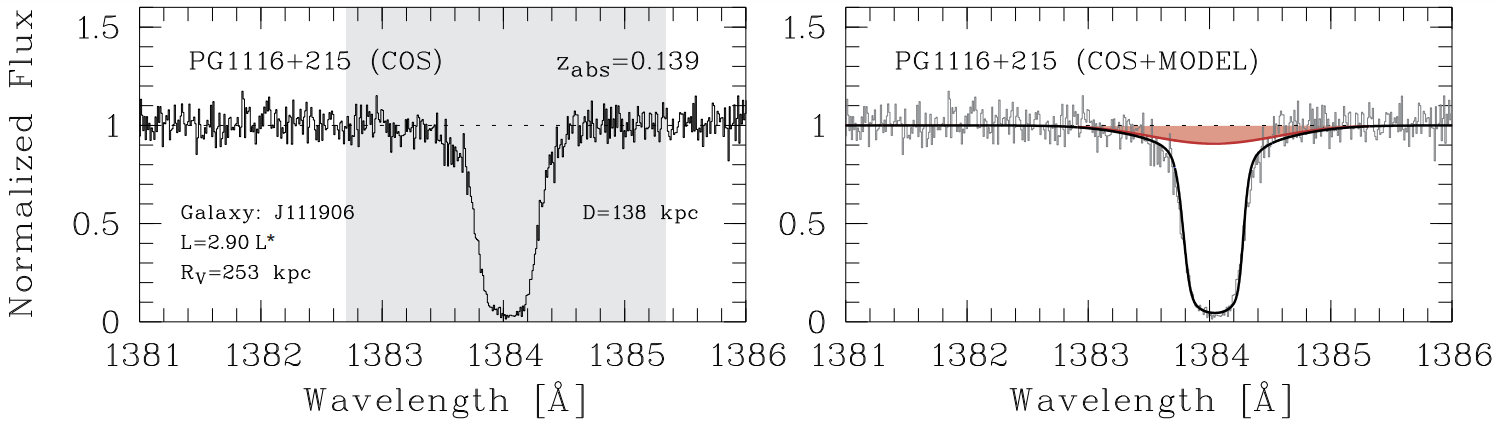
\includegraphics[width=\linewidth]{Figures/BLA.png}
    \caption{A BLA blended with other Ly$\alpha$ absorption lines towards the LOS of quasar PG1116+215 $(z_{em} = 0.176)$. Credits : \citet{Richter_2020}}
    \label{fig:BLA}
\end{figure}

There have been studies of BLAs on small scales but as these are difficult to observe they show varying results. For instance, \citet{Lehner-2007} have studied 7 AGN lines of sight to search for BLA candidates and estimated that BLAs contribute around 20\% to the total baryonic energy density ($\Omega_b$). However, a study by \citet{Danforth_2010}, which also studied 7 AGN lines of sight, report different results. They estimate the contribution of BLAs to be around 14\% in ($\Omega_b$).

So, there is a need to do a large survey of these BLAs to realise the abundance of baryons in these cosmic reservoirs. 

\section{Road-map for the Current Project}

In the current project we will be addressing the missing baryon problem with the help of BLAs. Currently, literature lacks comprehensive surveys of the BLAs on large datasets. So we will be doing a large survey of BLAs with high S/N HST/COS data. We will be modelling the ionisation conditions in the BLAs to infer their ionisation states. Our work will also include studying the galaxy environments of these BLA candidate systems to infer their origins. And then we would estimate the contribution of BLAs to the total cosmic baryonic inventory ($\Omega_b$). 

The outline of this report is as follows : In chapter \ref{chap:data}, we describe the data which we will be using for our survey of BLAs. In chapter \ref{chap:VPFIT} we mention our Voigt profile fitting routine. Chapter \ref{chap:Ion-Model} describes the ionisation modelling of the absorbers and the method used for modelling. In chapter \ref{ch:PG0003}, we study a BLA candidate absorber system towards the LOS of quasar PG 0003+158 to test our methods. Chapter \ref{ch:Survey} details the plan for our survey and partial results from the survey and we conclude by the reporting the future work in chapter \ref{ch:Thesis-Phase-II}. 

\chapter{Data and Pre-processing}  \label{chap:data}

\section{HST/COS data}

To detect BLAs we require very high S/N spectroscopic data of the background quasars. As we aim to the probe the WHIM at low redshift and at low redshifts the Lyman-$\alpha$ and other Lyman transitions fall in the Far Ultra-Violet (FUV) region of the electromagnetic spectrum. So we need FUV data for our study. 

We use FUV data from Cosmic Origins Spectrograph (COS) aboard Hubble Space Telescope (HST) as it provides us with highest S/N data compared to other FUV spectrographs like Space Telescope Imaging Spectrograph (STIS) which is also aboard HST. We use observations done in the FUV channel of COS with G130M and G160M gratings. The G130M grating gives a coverage of 900-1450 \AA \ with resolving power (R) of around 12,000-16,000, whereas G160M grating samples the wavelength between around 1360 and 1775 \AA \ and provide a resolving power of around 13,000-20,000. Together these gratings give coverage from around 1130 to 1790 \AA \ with a median resolution of R $\sim$ 17,000 (17.6 km s$^{-1}$).

The FUV detector of the COS comprises of two segments viz. A and B. This results in gap in the spectra of objects under observation. G130M and G160M gratings give a gap of 14.3  and 18.1 \AA \ respectively. To overcome these gaps, different central wavelength settings are used for observations so that there are overlaps in the spectrum thus covering the gaps. The COS FUV data can be accessed through the Hubble Spectral Heritage Archive (HSLA)\footnote{https://archive.stsci.edu/missions-and-data/hsla} which provides all the raw and integrated COS FUV data publicly available in the Mikulsky Space Telescope Archive (MAST)\footnote{https://archive.stsci.edu/}. The HSLA hosts the observations of 799 quasars, AGNs and Seyferts.
\\\\
\citet{danforth-2016} has surveyed the low redshift IGM with the highest quality HST/COS data available in the HSLA. They have chosen 82 UV-bright AGNs with redshifts $z_{AGN}<0.85$ and spectra with typical S/N ratio $\gtrsim$ 15 per COS resolution element. We use these 82 lines of sight for our study.  

\section{Pre-processing}

% \subsection{Continuum fitting}

The HST/COS data is over-sampled at 6 pixels per resolution element, so we re-sample the spectrum at an optimum binning of 2 pixels per resolution element. We use python package \emph{LINETOOLS}\footnote{https://github.com/linetools/linetools}, which uses simple linear interpolation and flux conservation, to rebin the spectrum. 
\\
A continuum is fitted to the spectrum after rebinning. To fit the continuum we again use the \emph{LINETOOLS} package, which places the knots at regions with no absorption and emission features at uniform spacing in wavelength along with interactive human input. The continuum is created by interpolating these knots with lower order polynomials. Then the spectrum is normalised by this continuum for fitting the Voigt profiles to the absorption lines.  









\chapter{Voigt Profile Fitting}  \label{chap:VPFIT}

\section{Voigt Profile}

The spectral lines are not infinitesimally peaked functions but rather have finite widths. This finite width or broadening can be attributed to the thermal motions of atoms (thermal broadening), quantum mechanical uncertainties in the energies of the transitions (natural broadening), collisions between excited atoms (collision broadening), etc. In astrophysical spectra the broadening is mainly thermal and natural broadening, the former results in Gaussian profile of the line whereas later gives a Lorentzian feature to the line profile. The convolution of these Gaussian and Lorentzian profiles results in what is known as the Voigt profile. The central region of an absorption line has a Gaussian shape whereas the extended wings show Lorentzian shape. So the absorption line in an astrophysical spectra can be modelled as Voigt profile. 
\\\\
The absorption profile at frequency $\nu$ can be written as:
\begin{equation*}
f(\nu)=f_{c} \ e^{-\tau(\nu)}
\end{equation*}
where $f, \ f_{c}, \ \tau$ are spectral flux density, interpolated absorption-free continuum over the absorption profile and optical depth respectively.

If we assume that the absorbing atoms have a Gaussian velocity distribution with mean velocity $v_0$ with respect to a reference frame, say S, then the optical depth is given by:

\begin{equation}  \label{eqn:tau}
\tau(\nu)=N \frac{1}{\sqrt{\pi}b}\int_{-\infty}^{\infty}\sigma(\nu')\ e^{-\frac{(v-v_0)^2}{b^2}} \text{d}v 
\end{equation}
where $N$ is the column density, $b$ is the Doppler parameter, which is defined as $b=FWHM/2\sqrt{ln2}$; $FWHM$ is the full width at half maximum and $\sigma(\nu')$ is the cross-section offered by an atom moving with the velocity $v$ to the photon of frequency $\nu$ in S and $\nu'=\nu/(1-v/c)$, taking $v$ to be positive for atoms receding away from the observer.  

The Doppler parameter $b$, has contributions from both thermal and non-thermal components (e.g. turbulence, etc.), which can be written as :
\begin{equation}
b=\sqrt{{b_{thermal}^2+b_{non-thermal}^2}}
\end{equation}
And $b_{thermal}$ is related to temperature (T) of the gas by $b_{thermal}=\sqrt{\frac{2kT}{m}}$, where $m$ is the mass of an atom and $k$ is the Boltzmann constant.
\\
We can get expression for cross-section in an atomic transition from the classical expression by taking in the factors of oscillator strength $(f)$ and frequency dependence which results from the finite life-time of the upper level of the transition. This expression is given by:
\begin{equation} \label{eqn:sigma}
\sigma=f \times \frac{1}{4\pi\epsilon_0} \frac{\pi e^2}{m_ec} \times \frac{1}{\pi} \frac{\frac{\gamma}{4\pi}}{{(\nu-\nu_0)}^2+{\frac{\gamma}{4\pi}}^2}
\end{equation}
where $\gamma$ is the total damping constant (de-excitation rate of the upper level) and other symbols have their usual meanings for the fundamental constants \citep{Voigt-eqn}. 
\\
Using equations \ref{eqn:sigma} \& \ref{eqn:tau} and changing frequency ($\nu$) to wavelength ($\lambda$) and putting values of the fundamental constants we get:

\begin{equation} \label{eqn:tau-lambda}
\tau(\lambda)=1.498 \times 10^{-2} \frac{Nf\lambda}{b} H(a,u)    
\end{equation}
where $H(a,u)$ is called the Voigt function and given as :
\begin{equation} \label{eqn:Voigt-func}
    H(a,u)=\frac{a}{\pi} \int_{-\infty}^{\infty} \frac{e^{-y^2}}{{(u-y)}^2+a^2} \text{d}y; \ a=\frac{\lambda \gamma}{4\pi b}; \ u=-\frac{c}{b}\left((1+\frac{v}{c})-\frac{\lambda}{\lambda_0}\right) 
\end{equation}
And $\lambda_0$ is the wavelength at the centre of the absorption profile. Clearly, the Voigt function is a convolution of gaussian and lorentizian functions. The absorption feature which is just $e^{-\tau(\lambda)}$, is called a Voigt profile.
\\\\
Figure \ref{fig:Voigt-b} shows simulated Voigt profile absorption lines with varying Doppler parameters at a fixed column density of $10^{13}$ cm$^{-2}$. It is evident from the figure \ref{fig:Voigt-b} that as the $b$ value increases the profile gets broader and shallower. So we require a very high S/N data to detect such shallow absorption features. Also, the optical depth at the center of the line decreases as $b$ increases. 

\begin{figure}[!h]
    \centering
    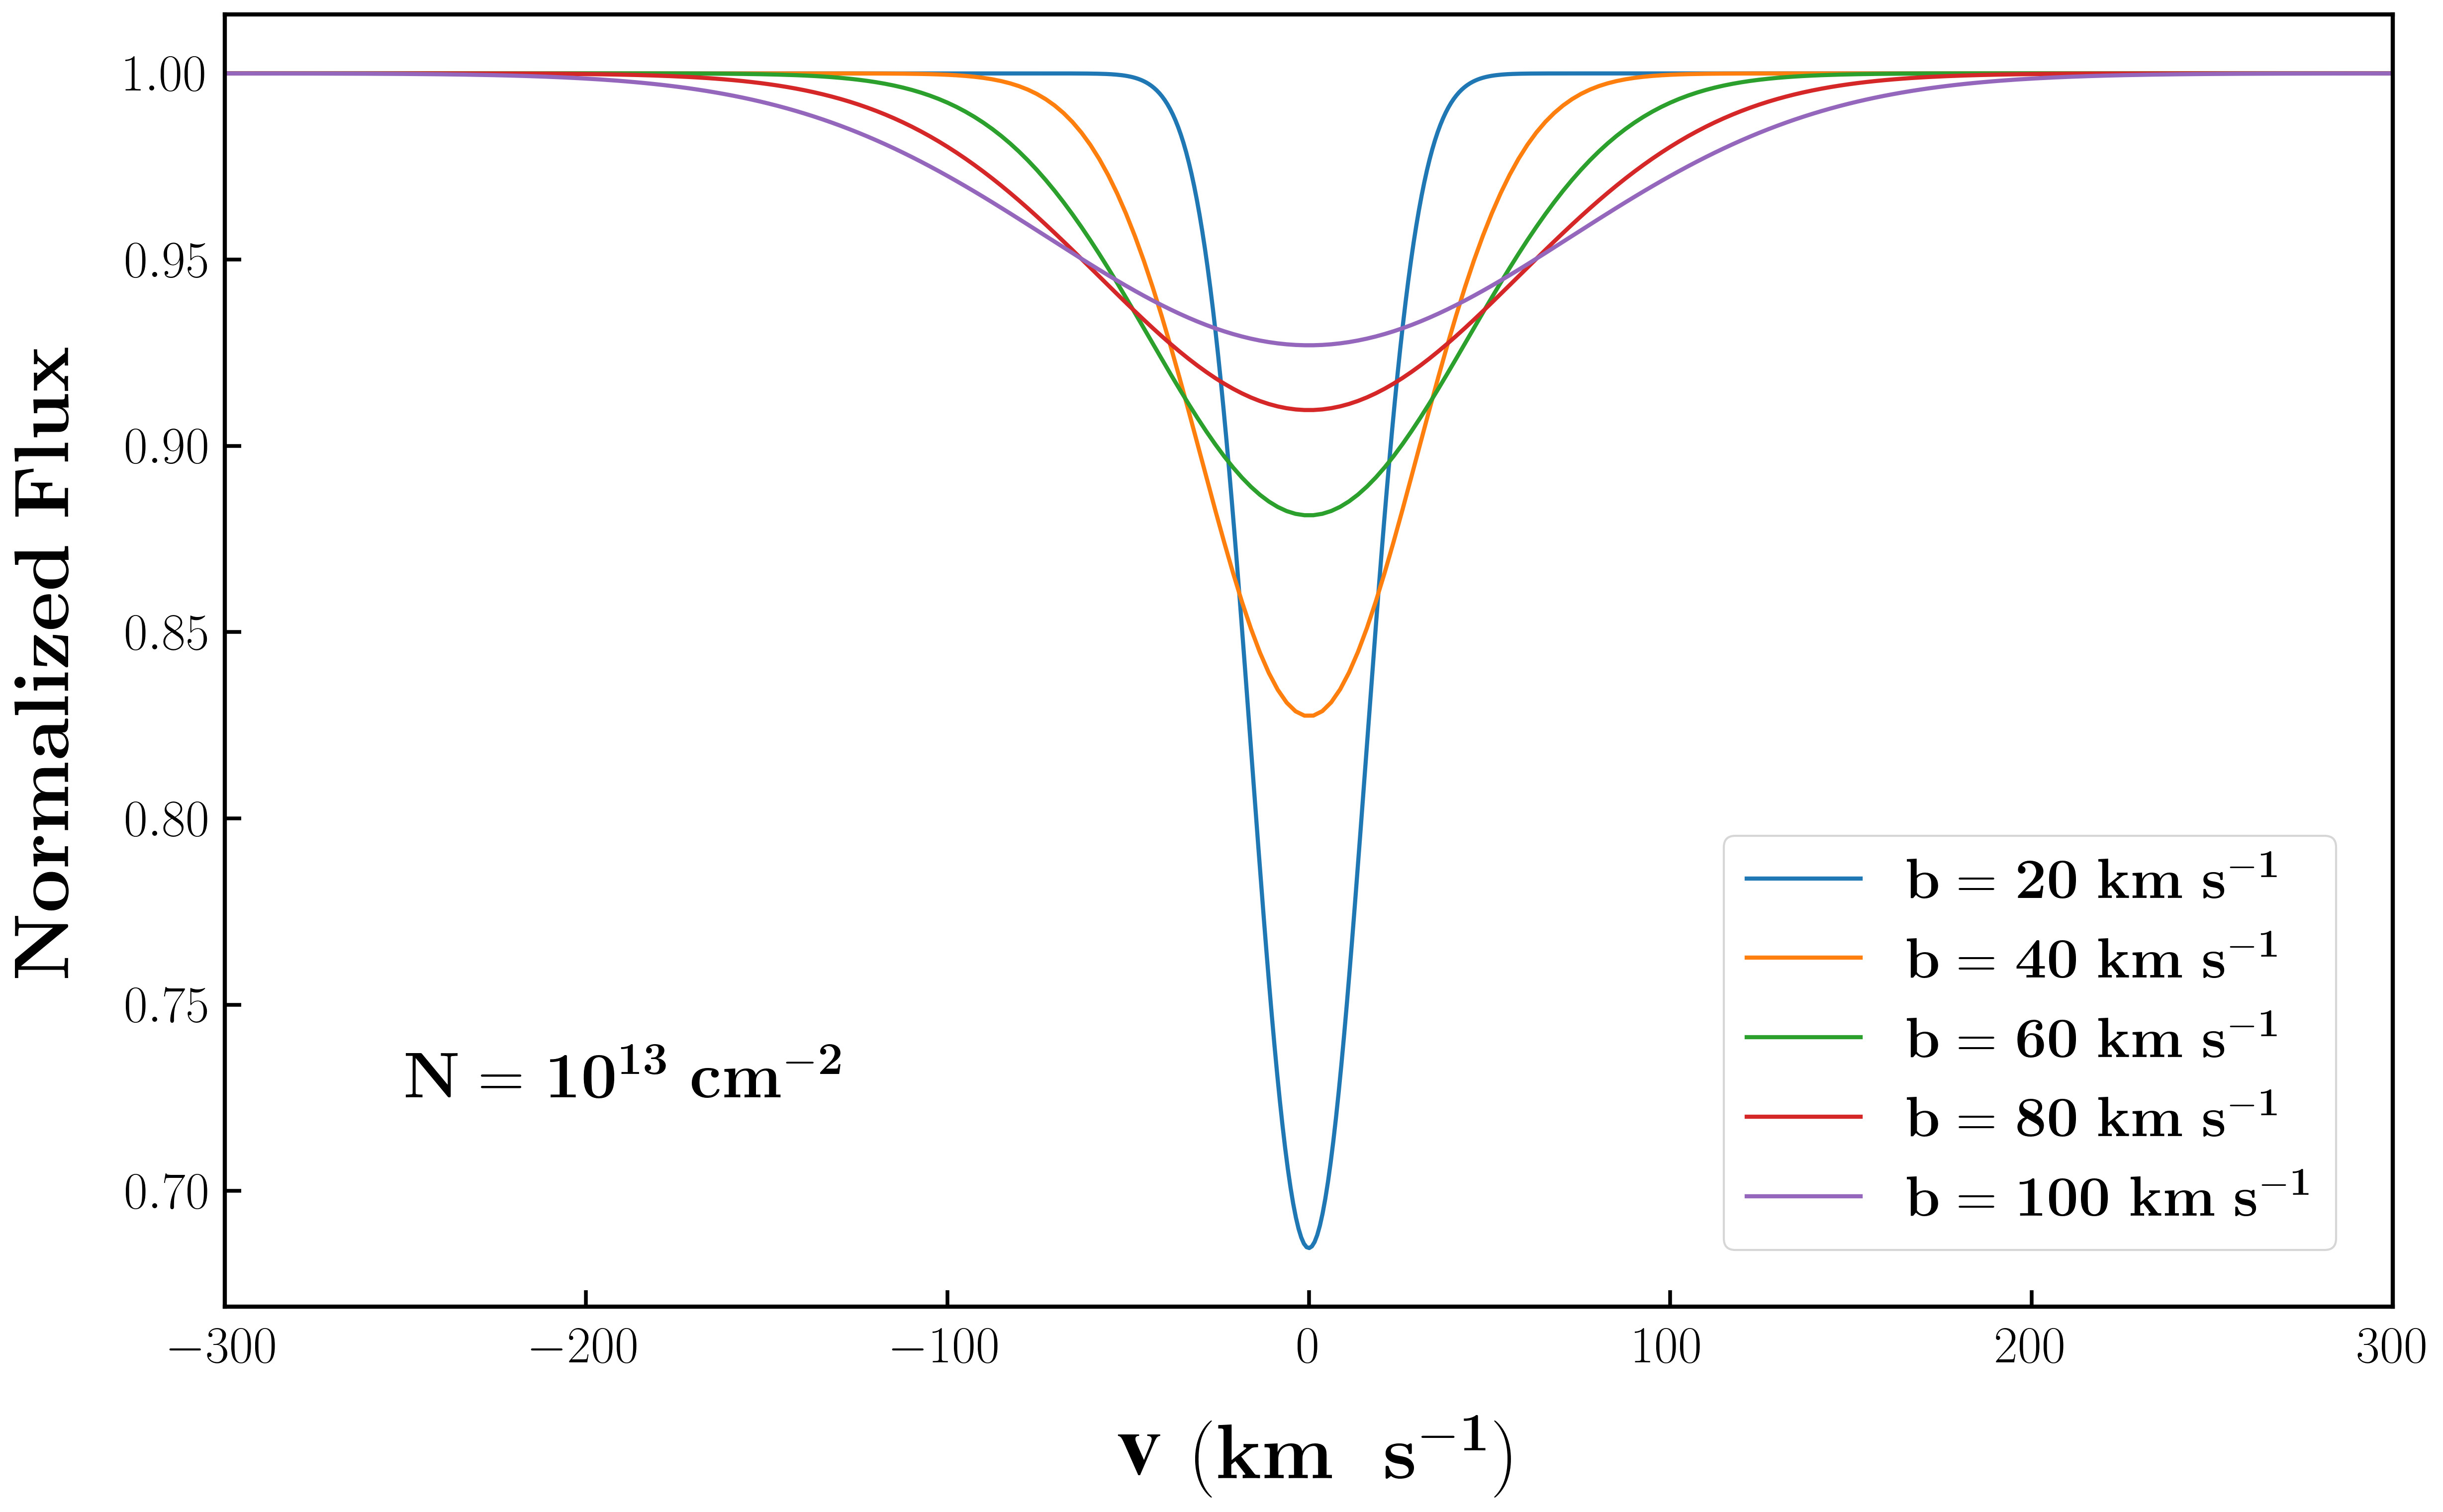
\includegraphics[width=\linewidth]{Figures/Voigt-b.jpg}
    \caption{Simulated Voigt profiles for different Doppler parameters. X-axis is the velocity from the central wavelength, taken as a proxy of wavelength}
    \label{fig:Voigt-b}
\end{figure}

Whereas figure \ref{fig:Voigt-N} shows the variation of Voigt absorption profile with column densities at a fixed Doppler parameter of 50 km s$^{-1}$. Now, as the column density increases, the optical depth at the center of the line increases resulting in the drop in flux, finally leading to the saturation of the profile, i.e. flux dropping to 0. Further increase in column density leads to the spread of profile and absorption from the wings also starts becoming prominent.

\begin{figure}[!t]
    \centering
    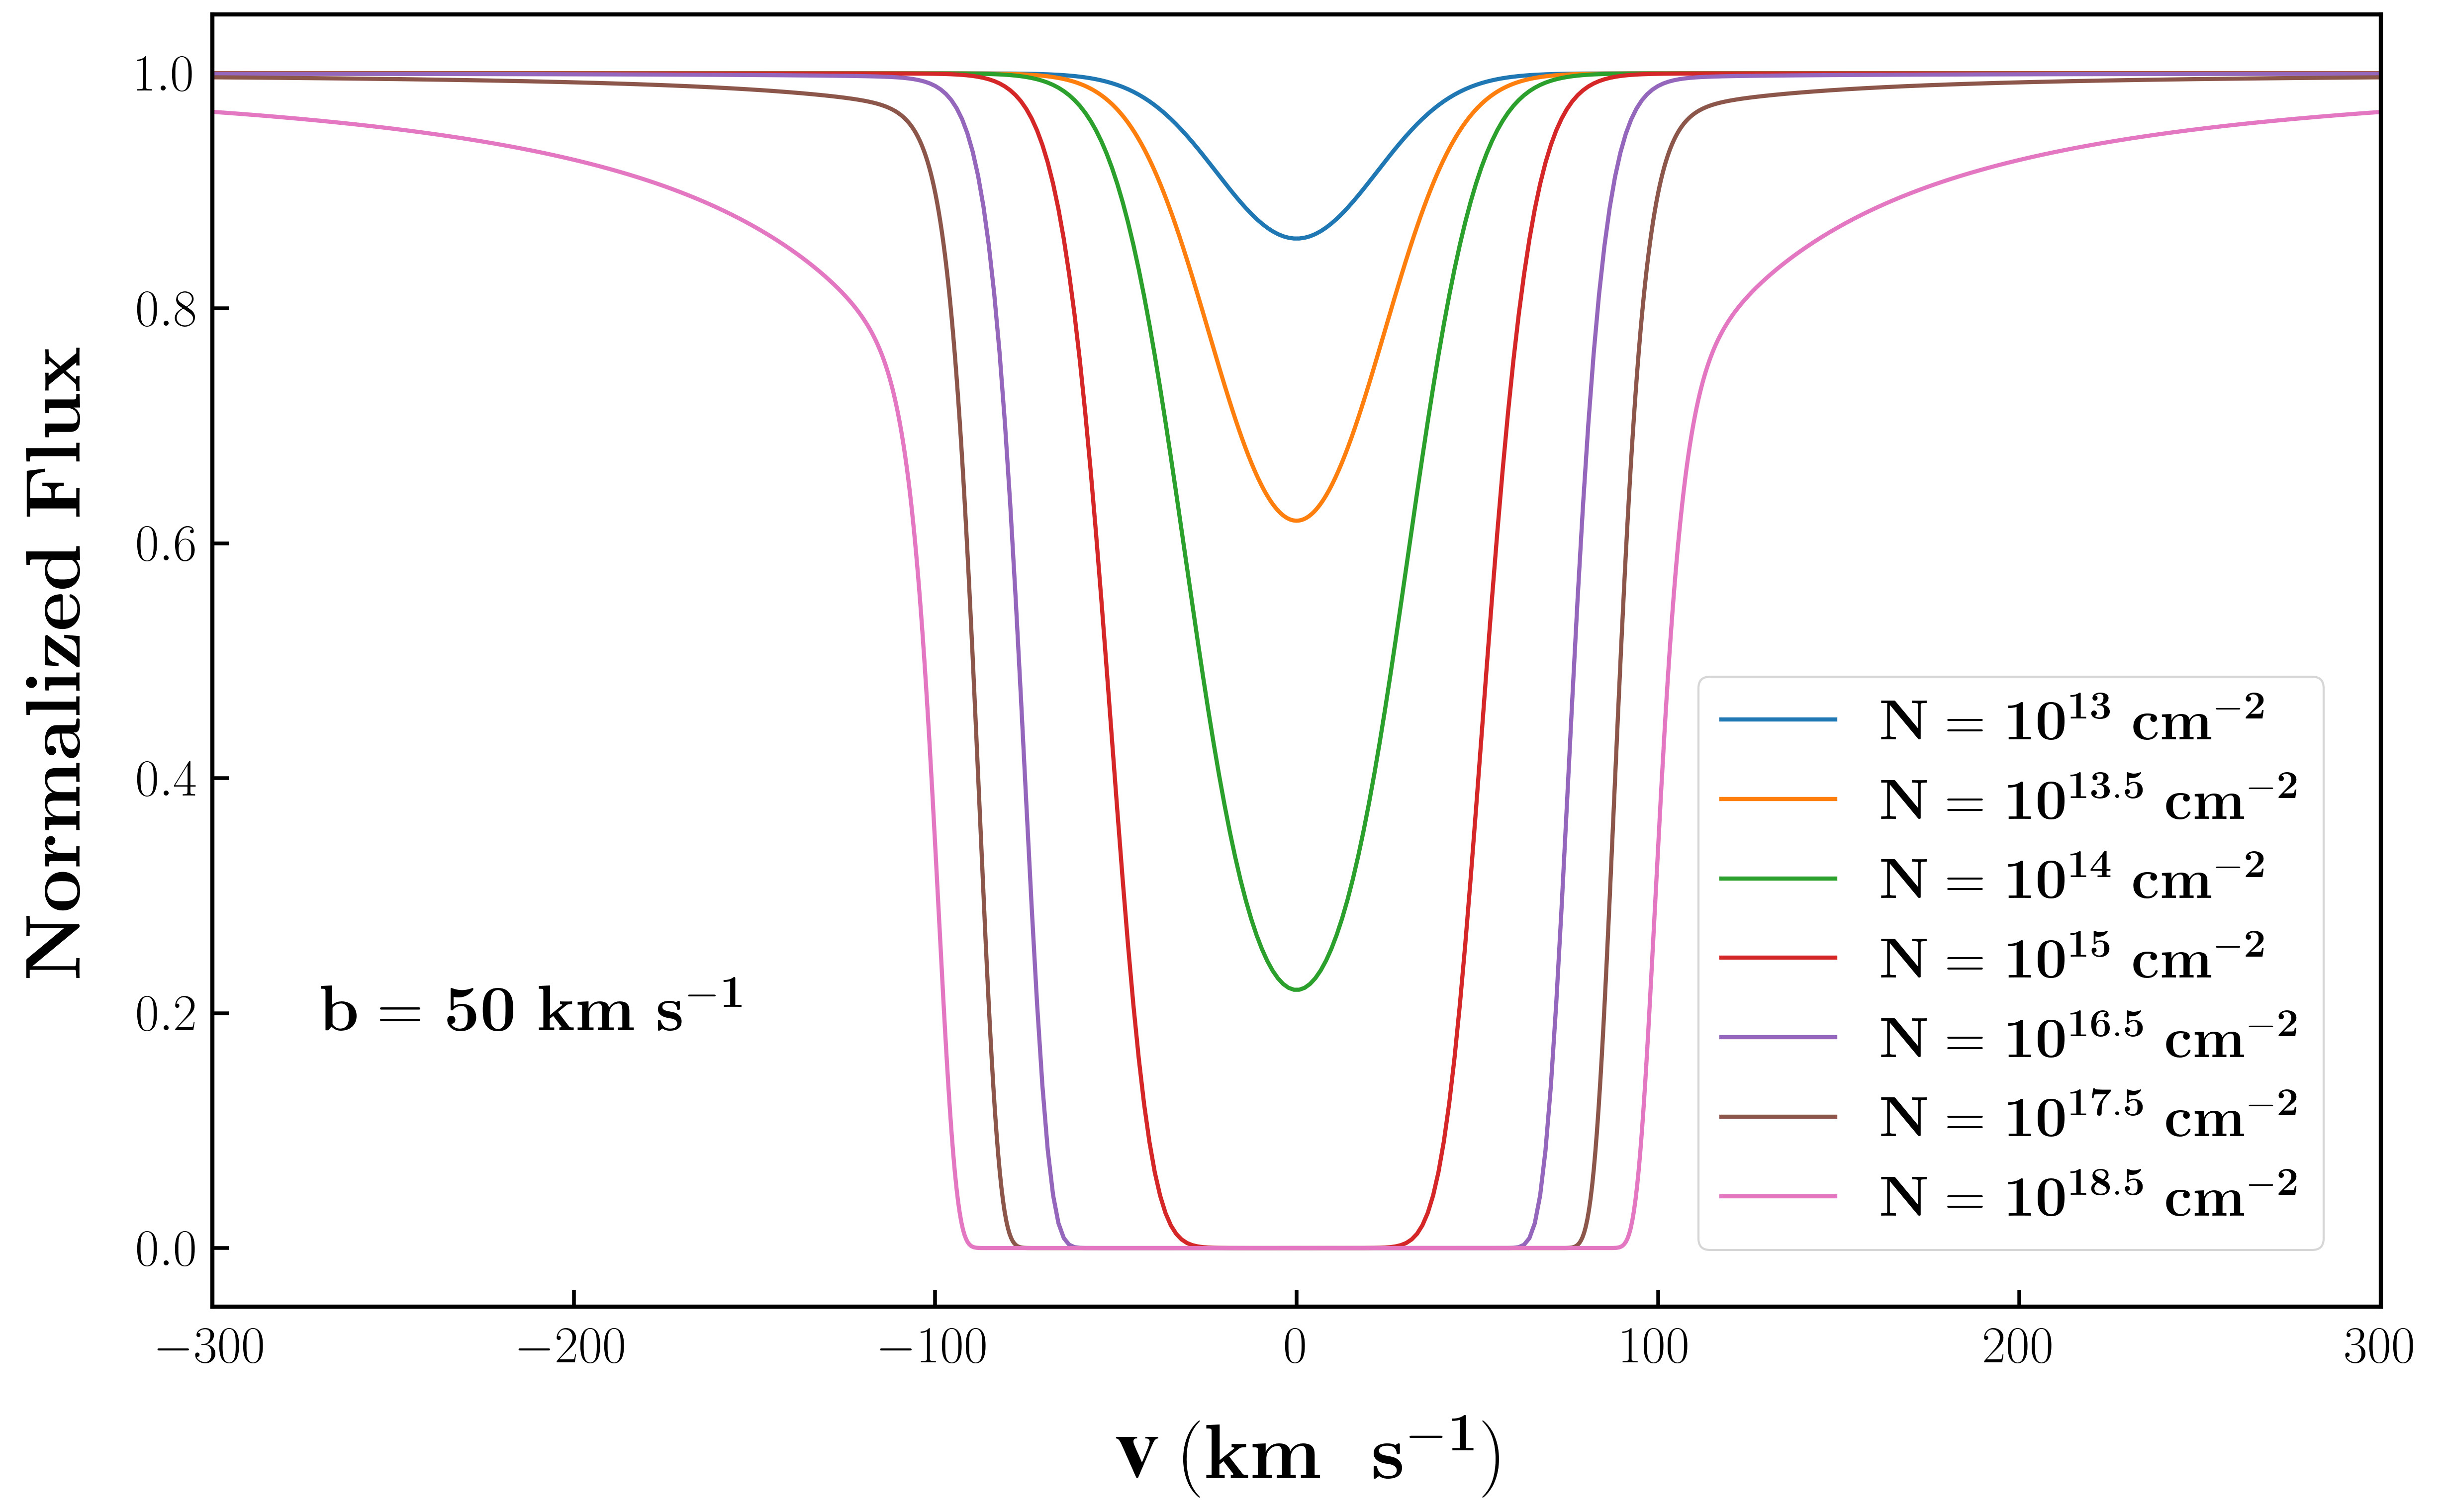
\includegraphics[width=\linewidth]{Figures/Voigt-N.jpg}
    \caption{Simulated Voigt profiles for different column densities. X-axis is the velocity from the central wavelength, taken as a proxy of wavelength}
    \label{fig:Voigt-N}
\end{figure}


\section{VPFIT}

Fitting Voigt profiles to the absorption lines in the spectrum of quasars is a very tedious task. The absorption lines can have the blend of multiple components of the same line or can be contaminated from some other line falling in the absorption profile of the line of interest. Furthermore, the atomic data characterising the transitions have to be carefully used.  All such challenges can't be solved using simple curve fitting tools available. 
\\\\
To fit the Voigt profiles to the absorption lines, we use Voigt profile fitting program ({\tt VPFIT}) \citep{vpfit}, which is developed specifically to deal with the absorption lines in astrophysical spectra . {\tt VPFIT} minimises the $\chi^2$ by varying the parameters in the parameter space. It gives 3 parameters and associated 1-$\sigma$ errors for each profile viz. redshift of the line (wavelength at centre of the absorption profile) , Doppler parameter (\emph{b}) and column density of the ion causing the absorption. We give {\tt VPFIT} an input file mentioning the continuum normalised spectrum, the wavelength region(s) to fit, initial guesses for the parameters and the ion for which we are fitting the absorption line. It also has a provision to include the instrument profiles in the form of line spread function (LSF) files. If LSF files are given, it then convolves the instrument profile and Voigt profiles. We use \textit{HST}/COS LSF files available on the STScI website\footnote{https://www.stsci.edu/hst/instrumentation/cos/performance/spectral-resolution}. In {\tt VPFIT}, we give the instrument profile as the LSF file of wavelength which lies between the fitting region of the line, if LSF file for such wavelengths is not available we then give the nearest wavelength LSF file available to the fitting region wavelengths. {\tt VPFIT} can also fit multiple Voigt profiles to the absorption lines in case multiple components are seen in the absorption lines. An example of Voigt profile fitting using {\tt VPFIT} is describe in section \ref{sec:VPfit-example}.

\subsection{Line-identification}

\citet{danforth-2016} have identified all the IGM absorber systems along each of the 82 lines of sight selected by them. They have also done the line identification of all the lines in each of the 82 spectra along with preliminary line fitting. However, their line fitting is not rigorous enough to be considered for our project as our results significantly depend on the line parameters. They have fitted the lines arising from same ions separately, leading to different parameters for the same ion. In principle, all the lines coming from a particular ion should be fitted simultaneously with same profiles, e.g. all the Lyman transitions should be fitted together rather than fitting Ly$\alpha$, Ly$\beta$, etc. alone. This helps us to better constrain the line parameters. For our fitting routine we use the line identification done by \citet{danforth-2016} and use their results as initial guess for our fitting procedure.

\vfill

\subsection{Example}  \label{sec:VPfit-example}

Figure \ref{fig:VPFIT-fit} shows an example of fitting a Voigt profile to an absorption line using {\tt VPFIT}. Figure \ref{fig:VPFIT-ip} gives the snapshot of an {\tt VPFIT} input file. In the first line we specify the continuum normalised spectrum (\emph{pks0405\_cont\_norm.asc}) and give a wavelength region where the profile is to be fitted in units used in the spectrum (\emph{1138.8 - 1141.4}) and we also give the LSF file as argument to \emph{pfinst}. In the considered example, we fit the line with two \ion{C}{iii} components by giving initial guesses of redshift (\emph{0.166588} \& \emph{0.167018}), Doppler parameter (\emph{39.7} \& \emph{35.3}) and column density (\emph{13.51} \& \emph{14.42})
 
The figure \ref{fig:VPFIT-op} shows the output file from {\tt VPFIT}. It gives us various statistics of the fit like number of iterations used (\emph{10}), reduced $\chi^2$ (\emph{1.380970}), etc. and the fitted line parameters and their 1$\sigma$ error.

It also displays the fit of the line as given in figure \ref{fig:VPFIT-fit}. The white step curve is the input spectrum and the green curve is the fitted Voigt profile. It shows that two components of \ion{C}{III} 977 line are fitted. It also allows us to save the fit in a separate file allowing further analysis on the data.


\begin{figure}[!htbp]
    \centering
     \begin{subfigure}[t]{\textwidth}
         \centering
         {
            \setlength{\fboxsep}{0pt}
            \setlength{\fboxrule}{1pt}
            \fbox{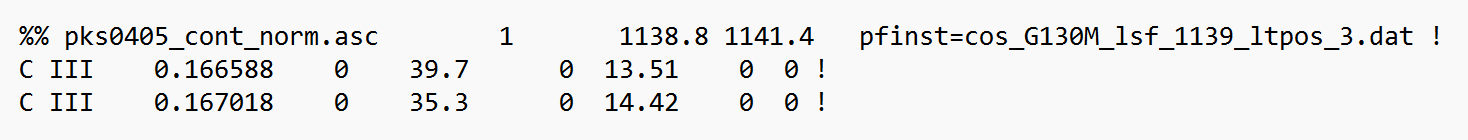
\includegraphics[width=\textwidth]{Figures/VPFIT_ip.png}}
}
         \caption{An example input file to {\tt VPFIT}}
         \label{fig:VPFIT-ip}
     \end{subfigure}

\medskip
\medskip
\medskip

    \begin{subfigure}[t]{\textwidth}
         \centering
         {
            \setlength{\fboxsep}{0pt}
            \setlength{\fboxrule}{1pt}
            \fbox{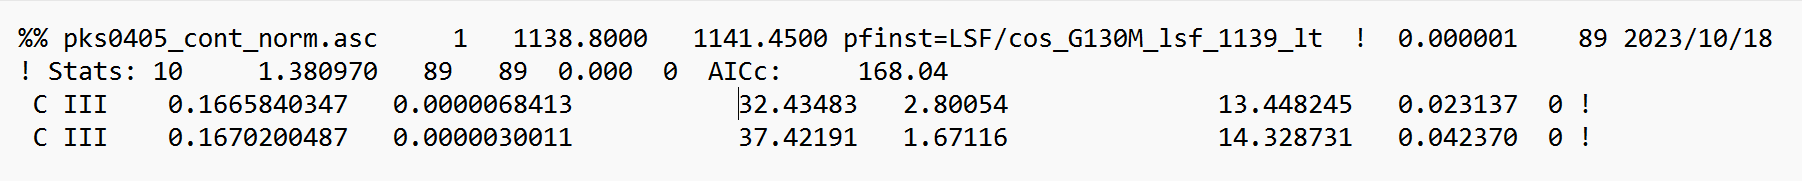
\includegraphics[width=\textwidth]{Figures/VPFIT_op.png}}
}
         \caption{An example output file from {\tt VPFIT}}
         \label{fig:VPFIT-op}
     \end{subfigure}
    \caption{Input to {\tt VPFIT} and output from {\tt VPFIT}}
    \label{fig:ip-op}
\end{figure}

\newpage

\begin{figure}[!t]
    % \vspace{-75mm}
     \centering
     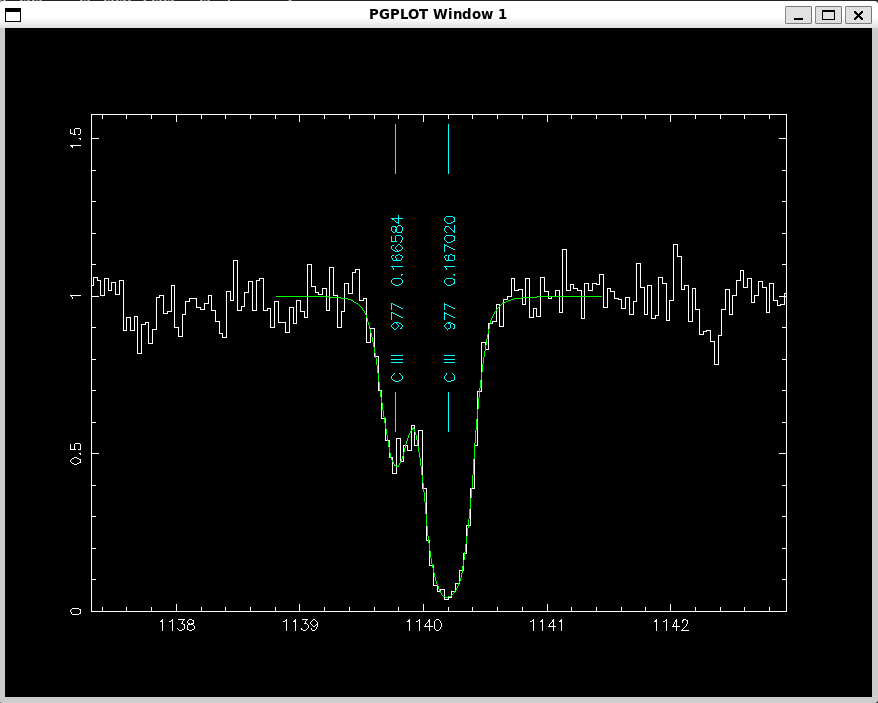
\includegraphics[width=0.8\textwidth]{Figures/VPFIT_fit.png}
     \caption{An example 2 component fit as displayed in {\tt VPFIT}}
     \label{fig:VPFIT-fit} 
\end{figure}

We use {\tt VPFIT} to fit the Voigt profiles to the absorption lines as described in this chapter. We use the column densities and Doppler parameters from Voigt profile fitting to model the ionisation conditions in the absorbers as described in next chapter.  
\chapter{Modelling the Ionisation Conditions}  \label{chap:Ion-Model}

\section{Ionisation  Modelling}

Relying solely on Voigt profile measurements yields limited information about the absorbers. It gives us the Doppler parameter, which can be used at best to put an upper level on the temperature of the absorbing gas. We need to know the physical conditions underlying in the absorber cloud such as density, temperature, metallicity, etc. As discussed in chapter \ref{chap:intro} that we need to show that the BLA is arising from a collisionally ionised phase, so that we can assure that we are indeed probing the WHIM and not just cool photoionised gas. And by modelling the ionization conditions prevalent in the absorber cloud we can address the aforementioned concerns.

\section{CLOUDY} \label{sec:Cloudy}

To model the ionization conditions prevailing in the absorbers, we use ionization modelling code CLOUDY \citep{cloudy}. CLOUDY considers processes like ionization, recombination, dissociation, and various chemical reactions among atoms, ions, and molecules. These processes determine the composition and abundance of different species in the absorber cloud. CLOUDY accounts for the radiation transfer within the gas cloud. This includes the absorption, emission, and scattering of photons. The simulation considers how radiation interacts with the particles in the cloud, influencing its temperature, density, and ionization state. 

It calculates the ionization equilibrium within the cloud, balancing ionization and recombination processes. It can perform equilibrium calculations for both photoionization and collisional ionization separately and simultaneously as well. To perform photoionization equilibrium calculations we give a model of extragalactic ionization radiation background, which mainly arises from AGNs and star formation activities, whereas for collisional ionization calculations we specify a temperature and then calculations are performed at this constant temperature. A combination of both will give results considering both types of ionizations simultaneously, such models are called hybrid models. 

CLOUDY takes various input parameters like density, temperature, redshift, metallicity of the cloud, abundance pattern of the elements, background radiation model, etc. to perform the equilibrium calculations. It models the clouds as plane parallel slabs with uniform densities and metallicities, and continues to add such slabs until a given stopping criteria is met. As we have the neutral Hydrogen column density from Voigt profile fitting, we use it as stopping criteria for CLOUDY simulations. So CLOUDY continues to add the slabs until the column density of neutral Hydrogen in simulated clouds reaches our given value.
Figure \ref{fig:Cloudy} shows the schematic of a CLOUDY simulation where neutral Hydrogen column density is used as a stopping criteria.
CLOUDY gives us a lot of useful quantities, including column densities and ionization fractions of various ions, equilibrium temperature (for photoionization calculations), etc. We can use these quantities to get the insights on the physical conditions and ionisation state of the absorbers. 

For all the CLOUDY models we set the abundance pattern of elements heavier than Helium to be that of solar abundance as given in \citet{grevesse-chemical-2010} and Helium abundance is set to $8.163\times{10}^{-2}$ (by number relative to Hydrogen) based on the latest CMB measurements \citep{planck_collaboration_planck_2020}. And for extragalactic radiation background model we use KS19 (Q18) model given in \cite{KS19}.  

\begin{figure}[!htbp]
    \centering
    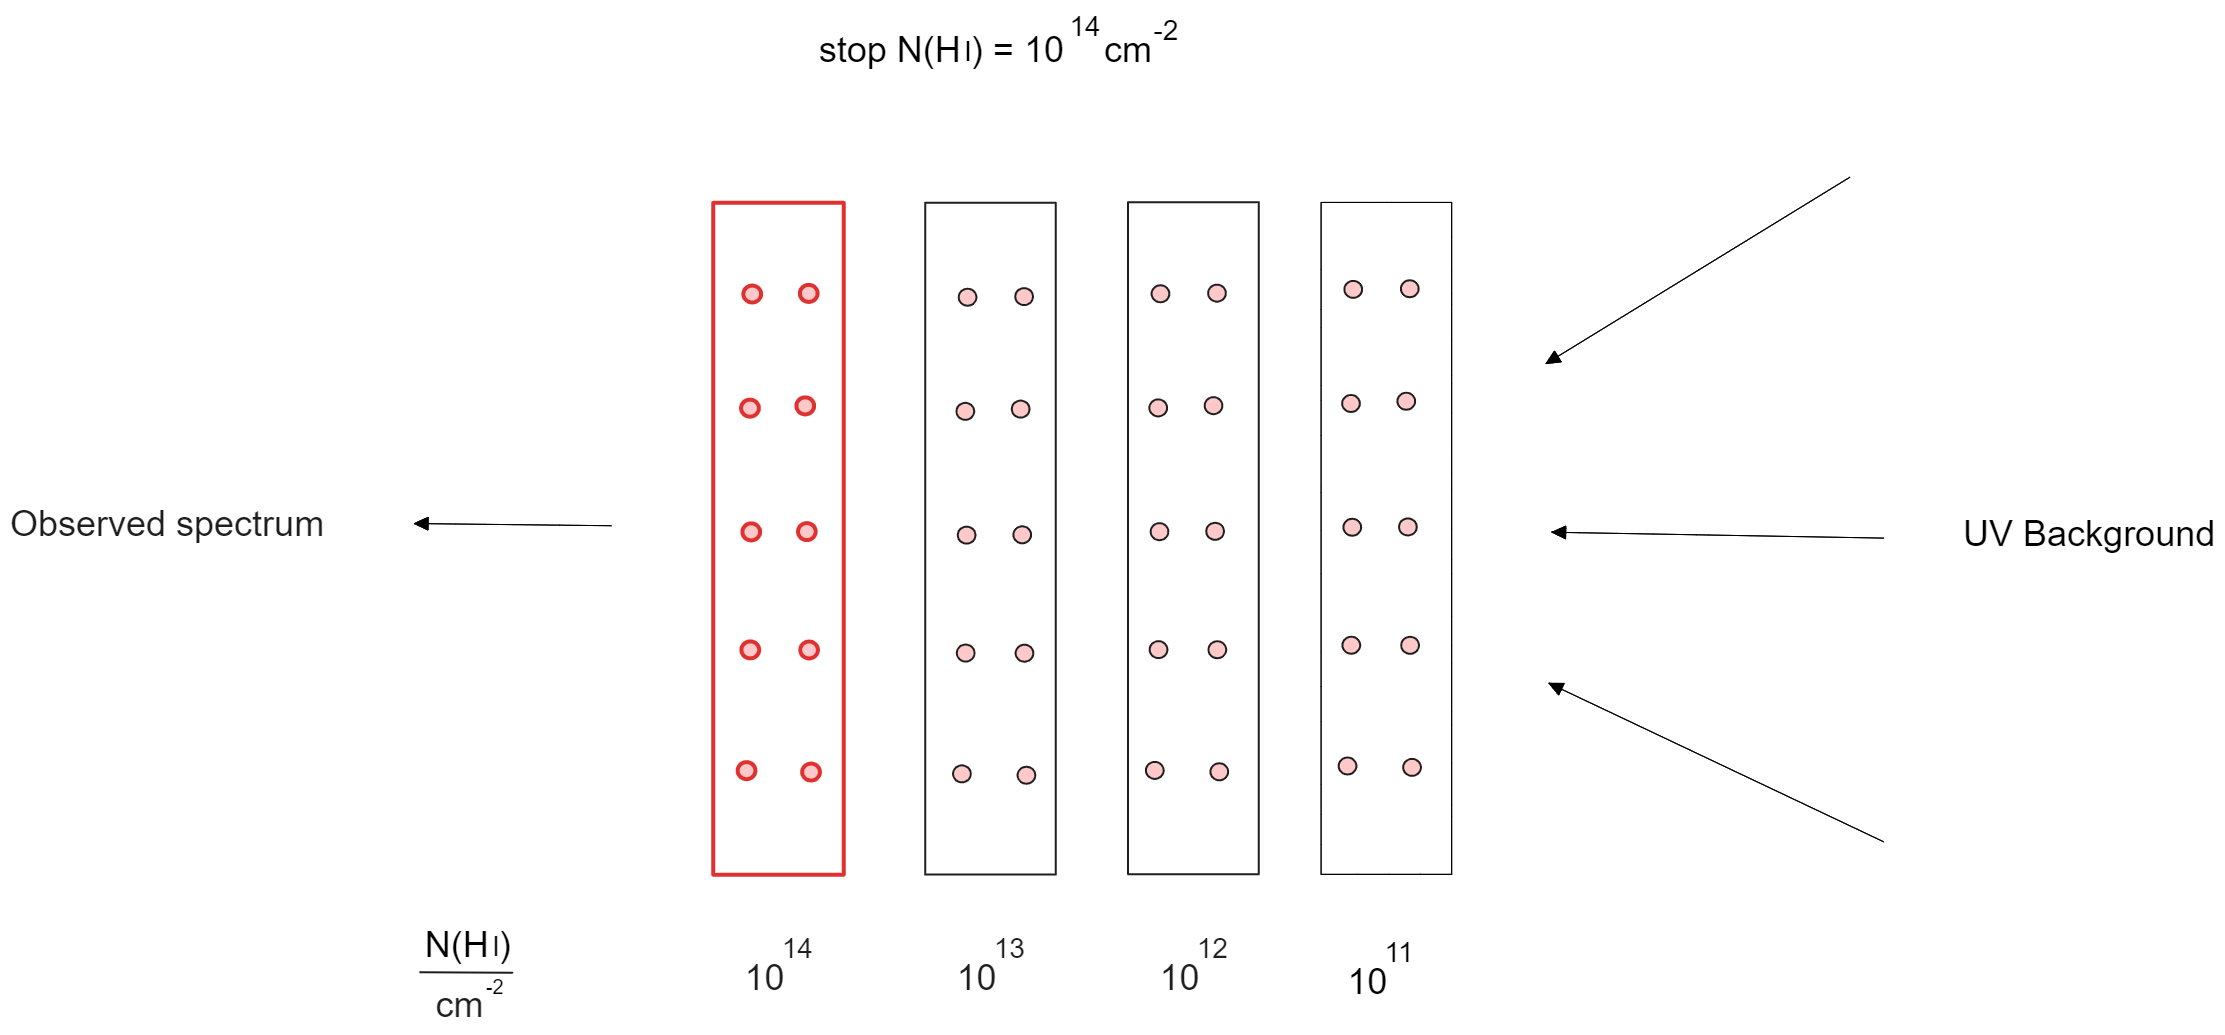
\includegraphics[width=\textwidth]{Figures/Cloudy.png}
    \caption{Schematic of a CLOUDY simulation.}
    \label{fig:Cloudy}
\end{figure}


\section{Ionization Model Based Parameter Estimation}  \label{sec:param-estimation}

As discussed in section \ref{sec:Cloudy}, we use CLOUDY to get the physical conditions existing in the absorber clouds. The physical conditions are characterised by properties like density, temperature, metallicity, pressures, etc. We estimate these quantities based on CLOUDY simulations with methods described in \citet{acharya_khaire}.

We use the $\chi^2$ minimisation technique as discussed in \citet{acharya_khaire} to estimate the density ($n_H$) and metallicity (Z) of the absorber. We consider a dense grid of photoionization CLOUDY models with varying the density ($n_H$) and metallicity (Z) over certain range in the parameter space. We give the  N(\ion{H}{i}) column density from Voigt profile measurements as the stopping criteria for the CLOUDY calculations. We interpolate the column densities in log $n_H$ and log Z space and then use $\chi^2$ minimisation to find the log $n_H$ and log Z values that best fits the data, i.e. the column densities of the observed ions. CLOUDY also gives us the equilibrium temperature also for all the density and metallicity. So we can find the temperature of the absorber cloud by putting the density and metallicity solution which we get from the above procedure. 

In case of collisional ionisation, we can follow the similar approach. If we can get a estimate of the temperature from some other means like using the Doppler parameters of the absorption lines, then we can use the same way of creating a 2D grid of CLOUDY models by fixing the temperature at the known temperature. When we give a constant temperature like this, CLOUDY performs collisional ionisation calculations. And if we don't know the temperature, then we can extend our 2D grid to a 3D one by varying the temperature also. And then use the same approach as in case of 2D grid to find the temperature as well.






\chapter{Absorber towards PG 0003+158} \label{ch:PG0003}

In this chapter, we describe a multi-component absorber system with a BLA candidate at $z\sim 0.347$ towards the line of sight of quasar PG 0003+158 ($z_{em}=0.4509$) which is a Sy1.2 AGN. We first fit the Voigt profiles to the absorption lines and then perform a detailed modelling of the ionization conditions in the absorber to know its ionisation state. We also analyse the galaxy neighbourhood of the absorber to understand the origins of the absorption system.   

\section{Component structure of the absorber system} \label{sec:component_structure}

We identified 3 components in the absorber system, i.e. three kinematically distinct absorption is seen. Table \ref{tab:components} lists the details of the components. We describe these components in subsequent sections.

\begin{table}
    \centering
    \begin{tabular}{ccc}
    \hline \hline 
    \head{Component}   &  \head{Ions} &  \head{$\mathbf{\Delta v \ (\text{km \ s}^{-1})}$} \\ 
    \hline \tabularnewline
         I    &                                     \ion{H}{i}                                       &   -163       \\
        II    &                             \ion{H}{i}, \ion{O}{vi}                                  &    0         \\ 
       III    &   \ion{H}{i}, \ion{O}{vi}, \ion{C}{ii}, \ion{C}{iii}, \ion{Si}{ii}, \ion{Si}{iii}    &    65        \\
    \tabularnewline \hline \hline \tabularnewline
    \end{tabular}
    \vspace*{-4mm}
    \caption{Component structure of the absorber system. Reference velocity at z = 0.347586}
    \label{tab:components}
\end{table}

\subsection{Component I : z $\sim$ 0.346776}

This component is the simplest of the 3 components as it is detected only in Ly $\alpha$ and Ly $\beta$ lines. Both the line are detected above 5$\sigma$ significance levels. This component lies at $\sim -180 \ \text{km s}^{-1}$ from the component II (from redshift of \ion{O}{vi} line : z = 0.347586). The other ions covered in COS coverage like \ion{N}{v}, \ion{C}{ii}, \ion{C}{iii}, \ion{Si}{ii}, \ion{Si}{iii}, \ion{Mg}{ii}, etc. are non-detections. Voigt profile fitting, as described in section \ref{sec:Voigt_fitting}, gives a \ion{H}{i} column density, \text{log N[\ion{H}{i} ($\text{cm}^{-2}$)]} = $13.46 \pm 0.05$ . The \emph{b} parameter measured from Voigt profile fitting gives an upper estimate of the temperature for the component to be $10^{{4.94}_{-0.16}^{+0.14}}$ K, assuming a complete thermal broadening of the line. 

\subsection{Component II : z $\sim$ 0.34758}

This component shows a number of Lyman lines from Ly $\alpha$ (23$\sigma$) to Ly $\delta$ (3.7$\sigma$) along with coincident absorption from \ion{O}{vi} at above 10$\sigma$ confidence level. The other ions in the COS coverage are non-detections. It hosts the Broad Lyman Absorber (BLA), having a \emph{b} parameter of $62.5 \pm 2.9 \ \text{km s}^{-1}$ and a column density of \text{log N[\ion{H}{i} ($\text{cm}^{-2}$)]} = $14.13 \pm 0.02$. The broad line indicates a large temperature. The temperature can be directly estimated using the \emph{b} values of \ion{H}{i} and \ion{O}{vi}, assuming that they both arise from same the gas phase. This gives a temperature of ${10}^{{5.29}_{-0.08}^{+0.07}}$ K (see section \ref{sec:temp_calc_b}) , which lies in the temperature range of WHIM $(10^5-10^7)$ K.   

\subsection{Component III : z $\sim$ 0.34790}

This lies at around 70 $\text{km s}^{-1}$ from the component II (from redshift of \ion{O}{vi} line : z = 0.347586). It is kinematically more complex than the other two components. Lyman transitions are seen upto \ion{H}{i} 914 {\AA} with \text{log N[\ion{H}{i} ($\text{cm}^{-2}$)]} = $16.10 \pm 0.02$ together with 5 ionized metal absorption lines in form of \ion{O}{vi}, \ion{C}{ii}, \ion{C}{iii}, \ion{Si}{ii} and \ion{Si}{iii}. Metal line absorptions allows us to model the ionizing conditions prevailing in the absorbing clouds with more reliability as discussed in section \ref{sec:ionization_modelling} to estimate the physical conditions of the absorber. 

\section{Voigt profile fitting} \label{sec:Voigt_fitting}

Lyman lines are seen in varying numbers in different components of the absorber system. To better constraint the line parameters, we fit all the Lyman transitions upto \ion{H}{i} 918 together. We exclude higher order Lyman lines than \ion{H}{i} 918 because of their weak S/N. The Ly $\beta$ has a contamination redward of the component III from Ly $\gamma$ at z=0.421883. \ion{O}{vi} 1032,1038 also shows two component structure. This doublet is fitted simultaneously with two components. \ion{Si}{ii} 1260 and \ion{Si}{iii} 1206 lines show single component structure and are fitted separately with single components. \ion{C}{ii} 1036 line shows a single component profile and hence fitted with one component. At first glance the \ion{C}{iii} 977 line looks like it has two component structure but it is contaminated from Ly $\alpha$ coming from z=0.083078, \ion{H}{i} 926 from z=0.421823 and \ion{H}{i} 926 from z=0.386036, 0.386295. So we fit this line with single \ion{C}{iii} component and these contaminations. 

The system plot for the absorber system is shown in figure \ref{fig:sys_plot} over-plotted with fitted Voigt profiles. Horizontal axis is the rest-frame velocity of lines with respect to z = 0.347586 (redshift of \ion{O}{vi} line of the component II) used as a proxy of wavelength and vertical axis represents the continuum normalized flux. The green step curve is the observed flux, the red solid curve is the Voigt profile fit, the blue dashed curves are the individual components that make the absorption profile with orange ones being the contamination (e.g in Ly$\beta$ and \ion{C}{iii} 977), the light pink step curve is the continuum normalized error in observed flux and the vertical blue ticks shows the position of each component. Fitted parameters are tabulated in table \ref{tab:fit_param}.

\begin{table}[!t]
\centering
\begin{tabular}{cccccc}
        \hline \hline
       \head{Line} & \head{Component} & \head{v (km s\textsuperscript{$\mathbf{-1}$})} & \head{b (km s\textsuperscript{$\mathbf{-1}$})} & \head{log [N cm\textsuperscript{$\mathbf{-2}$}]} 
       \tabularnewline \hline \tabularnewline 
\multirow{3}{*}{\ion{H}{i} 918-1215}   & I    & \hspace*{-4.5mm} -163 $\pm$ 4  & 38 $\pm$ 6 & 13.46 $\pm$ 0.05  \tabularnewline
                                       & II   & \hspace*{1mm} 1 $\pm$ 1  & 62 $\pm$ 3 & 14.13 $\pm$ 0.02 \tabularnewline
                                       & III  & 68 $\pm$ 1  & 16 $\pm$ 1 & 16.10 $\pm$ 0.02  \tabularnewline \tabularnewline

\multirow{2}{*}{\ion{O}{vi} 1032,1038} & II   & \hspace*{1mm} 0 $\pm$ 1  & 30 $\pm$ 2 & 14.26 $\pm$ 0.09    \tabularnewline
                                       & III  & 62 $\pm$ 1  & 13 $\pm$ 2 & 13.91 $\pm$ 0.04   \tabularnewline \tabularnewline   
\ion{C}{ii} 1036                       & III  & 64 $\pm$ 1  & \hspace*{3mm} 3 $\pm$ 28 & 
\hspace*{1mm} 14.21 $\pm$ 16.55   \tabularnewline \tabularnewline
\ion{C}{iii} 977                       & III  & 70 $\pm$ 1  & 23 $\pm$ 2 & 13.81 $\pm$ 0.04   \tabularnewline \tabularnewline
\ion{Si}{ii} 1260                      & III & 65 $\pm$ 1  & \hspace*{3mm} 3 $\pm$ 23 & \hspace*{1mm} 13.19 $\pm$ 12.32  \tabularnewline \tabularnewline
\ion{Si}{iii} 1206                     & III & 68 $\pm$ 2  & \hspace*{1.1mm} 10 $\pm$ 12 &  12.87 $\pm$ 1.19   \tabularnewline \tabularnewline \hline \hline \tabularnewline
    \end{tabular}
    \vspace*{-4mm}
    \caption{Parameters from Voigt profile fitting of the absorption lines. Velocity is taken to be zero at the redshift of \ion{O}{vi} line of component II, i.e. z = 0.347586}
    \label{tab:fit_param}
\end{table}

VPFIT gives overestimated errors in the column densities and \emph{b} values when the \emph{b} value is significantly less than the COS spectral resolution ($\approx$17 $\text{km} \ \text{s}^{-1}$) as can be seen for \ion{C}{ii}, \ion{Si}{ii} and \ion{Si}{iii} lines. So, we used $\chi^{2}$ of the fit to determine the uncertainties in the parameters. To do so, we fix all the parameters other than parameter whose uncertainty is to be determined. This free parameter is varied until $\chi^{2}$ increases by 1 unit. The absolute difference between this value of parameter and best fit parameter gives 1-$\sigma$ uncertainty in the parameter. We have one more source of uncertainty in the parameters, which manifests due to the continuum fitting, as the continuum fitting is subjective. To incorporate this uncertainty, we consider two more continuum, one at 3\% above and 3\% below the continuum used earlier. We again fit the lines, as described above to the spectrum normalised by these continuum.  The absolute difference in the parameters from these fit and earlier fit is taken as the systematic error in the parameters. To be conservative, we take maximum of the differences in the parameter values as systematic errors in the parameters and add them in the earlier errors. Table \ref{tab:col_den_error} gives the errors estimated in column densities using both the methods mentioned above.

\begin{table}[!ht]
    \centering
    
    \begin{tabular}{cccc}
            \hline \hline
           \head{Line}  & \head{Component}  & \head{$\mathbf{\chi^2}$}   &  \head{Continuum}  
           \tabularnewline \hline \tabularnewline  
            \multirow{3}{*}{\ion{H}{i} 918-1215} & I    & 0.04 & 0.07 \tabularnewline
                                                 & II   & 0.02 & 0.04  \tabularnewline
                                                 & III  & 0.02 & 0.03  \tabularnewline \tabularnewline
                                                   
            \multirow{2}{*}{\ion{O}{vi} 1032,1038} & II  & 0.02 & 0.03   \tabularnewline
                                                   & III & 0.03 & 0.01  \tabularnewline \tabularnewline
                                                   
            \ion{C}{ii} 1036        & III               & 0.20 & 0.19  \tabularnewline \tabularnewline
            \ion{C}{iii} 977        & III               & 0.03 & 0.01 \tabularnewline \tabularnewline
            \ion{Si}{ii} 1260       & III               & 0.25 & 0.16  \tabularnewline \tabularnewline
            \ion{Si}{iii} 1206      & III               & 0.06 & 0.02  \tabularnewline \tabularnewline \hline \hline \tabularnewline
            
        \end{tabular}
        \caption{Error calculated using $\chi^2$ and the systematic uncertainty in column densities due to continuum fitting given in units of log[N ($\text{cm}^{-2}$)]} 
        \label{tab:col_den_error}
    \end{table}
    

\begin{landscape}

\thispagestyle{empty}

\begin{figure}
\centering
\vspace{-10mm}
\hspace*{-20mm}
\captionsetup{oneside,margin={0cm,20mm}}
\includegraphics[width=1.1\linewidth]{Figures/PG0003+158_z=0.347586_sys_plot.png}
\caption{System plot of the absorption system. Reference velocity taken at $z=0.347586$}
\label{fig:sys_plot}
\end{figure}

\end{landscape}


% \begin{table}[!ht]
% \centering

% \begin{tabular}{cccc}
%         \hline \hline
%        \head{Line}  & \head{Component}  & \head{$\mathbf{\chi^2}$}   &  \head{Continuum}  
%        \tabularnewline \hline \tabularnewline  
%         \multirow{3}{*}{\ion{H}{i} 918-1215} & I    & 0.04 & 0.07 \tabularnewline
%                                              & II   & 0.02 & 0.04  \tabularnewline
%                                              & III  & 0.02 & 0.03  \tabularnewline \tabularnewline
                                               
%         \multirow{2}{*}{\ion{O}{vi} 1032,1038} & II  & 0.02 & 0.03   \tabularnewline
%                                                & III & 0.03 & 0.01  \tabularnewline \tabularnewline
                                               
%         \ion{C}{ii} 1036        & III               & 0.20 & 0.19  \tabularnewline \tabularnewline
%         \ion{C}{iii} 977        & III               & 0.03 & 0.01 \tabularnewline \tabularnewline
%         \ion{Si}{ii} 1260       & III               & 0.25 & 0.16  \tabularnewline \tabularnewline
%         \ion{Si}{iii} 1206      & III               & 0.06 & 0.02  \tabularnewline \tabularnewline \hline \hline \tabularnewline
        
%     \end{tabular}
%     \caption{Error calculated using $\chi^2$ and the systematic uncertainty in column densities due to continuum fitting given in units of log[N ($\text{cm}^{-2}$)]} 
%     \label{tab:col_den_error}
% \end{table}



\section{Ionization Modelling of the Absorber} \label{sec:ionization_modelling}
 
We have three components in our absorber system. But the first component has only \ion{H}{i} absorption lines, we can't get anything than the upper limit on the temperature for this component, ionization modelling can't be performed for this component. So detailed modelling is done for components II and III only as discussed in subsequent sections.

\subsection{Component II} \label{sec:compII_modelling}

For this component, we only have \ion{O}{vi} absorption other than \ion{H}{i} absorption. For modelling the ionizing conditions in this component we use very simplistic approach as we don't have much constraining parameters on the models. We consider both photoionisation and collisional ionisation scenarios for this component.

\subsubsection{Photoionization modelling}

Metallicity is an essential parameter for modelling the ionization conditions. But we cannot make an estimate of metallicity for this component directly. As this component and component III are separated by small velocity ($\approx$ 65 $\text{km} \ \text{s}^{-1}$), we assume that the metallicity change would not be significant between these components. So we take the metallicity of this component to be same as that of the component III, whose metallicity is estimated more rigorously as described in section \ref{sec:compIII_modelling}. To estimate the density, we run a grid of photoionization (PIE) CLOUDY models with varying log $n_H \ (\text{cm}^{-3})$ between -5 to 0 at steps of 0.02 and using the metallicity as what we get for the component III in section \ref{sec:compIII_modelling} and using log [N(\ion{H}{i}) (${cm}^{-2}$)] = 14.13 as stopping criteria. We then take the density of this component to be the density at which we recover the \ion{O}{vi} observed column density for this component.

As discussed in section \ref{sec:compIII_PIE}, we take the metallicity for this component to be what we get from excluding \ion{O}{vi} case of the component III photoionization modelling (see section \ref{sec:compIII_modelling}). Using this metallicity, we get the  density , log $n_H \ (\text{cm}^{-3})$ = $-4.51$ . The modelled column densities of other ions detected in component III (\ion{C}{ii}, \ion{C}{iii}, \ion{Si}{ii} and \ion{Si}{iii}) are in agreement with the upper limits based on non-detections obtained from apparent optical depth measurements. This solution predicts an equilibrium temperature of around $2.5\times 10^4$ K, which contradicts with the temperature obtained from \emph{b} value of \ion{H}{i} and \ion{O}{vi} by an order of magnitude as calculated in section \ref{sec:temp_calc_b}. The total hydrogen column density predicted by this solution is $\text{log [N(H)} \text{cm}^{-2}]$ = 18.45, which results in line of sight thickness of around 30kpc, which is physically unrealistic given that CLOUDY models the clouds to be homogeneous. Such large structures don't produce simple systems like what we observed. So we discard this solution to be depicting the prevailing conditions in the absorbing cloud. 

\subsubsection{Collisional ionization modelling}

We also perform a collisional ionization equilibrium (CIE) modelling for this component. We consider hybrid models where both photoionization (from ionizing extragalactic background) and collisional ionization are occurring simultaneously. We run a grid of CLOUDY models with varying the log $n_H \ (\text{cm}^{-3})$ from -5 to 0 with steps of 0.02 and log Z/$\mathbf{\text{Z}_{\odot}}$ from -3 to 2 with steps of 0.04 at a constant temperature of $10^{5.29}$ K, as calculated in section (temperature calculation). Though we have considered hybrid models, at these temperatures collisional ionisation would be a dominant process. We then find the metallicities where the observed \ion{O}{vi} column density matches the modelled column density for different log $n_H$ values.  
\\
We only have \ion{O}{vi} column density as a constraining parameter in these models. We also use size as a constraint to arrive at the conditions prevailing in the component. As we have fairly simple absorber with just Lyman and \ion{O}{vi} absorption, we profess that the size of the absorber must not be very large, since large absorber clouds would not produce such simple absorber systems. So we discard out the low density scenarios, as low density would result in large line of sight lengths to recover the observed column densities. This helps us to constrain the density as, log $n_H \ (\text{cm}^{-3})$ > -3 as viable conditions for the absorber cloud. As shown in figure \ref{fig:comp_II_CIE}, this corresponds to log Z/$\mathbf{\text{Z}_{\odot}}$ > 0.4 . Now we run a hybrid model with this density, metallicity at constant temperature of log T (K) = 5.29. This gives an upper limit on total  Hydrogen column density, $\text{log [N(H)} \ \text{cm}^{-2}]$ = 19.62, which results in an upper estimate on the size to be $\sim$13 kpc.
%
\begin{figure}[!t]
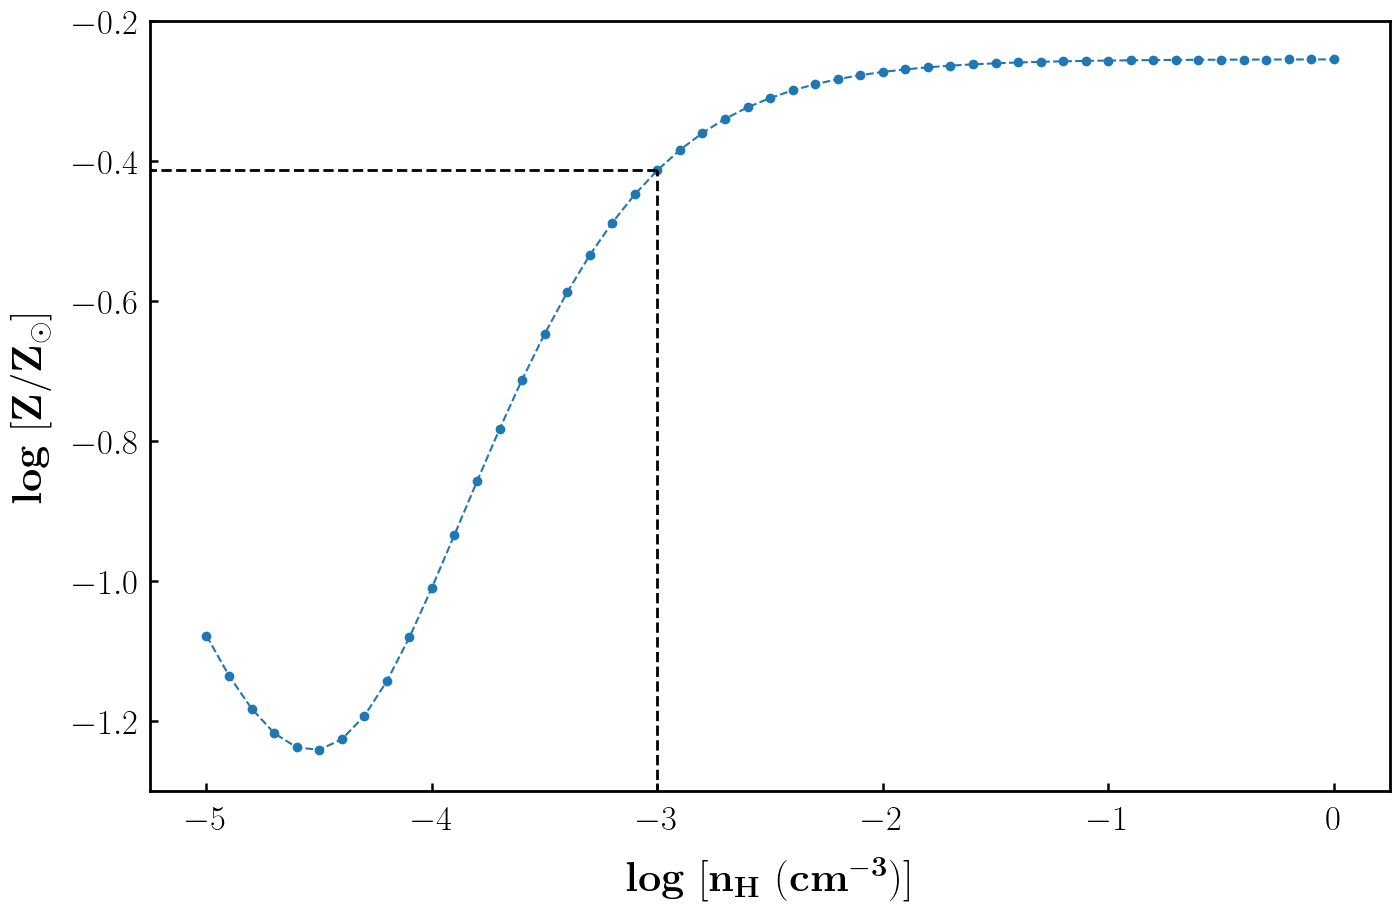
\includegraphics[width=\linewidth]{Figures/comp-II-CIE.png}
\caption{CIE solution for component II. The figure shows the metallicity found for various densities. At high densities no variation in metallicity is seen.}
\label{fig:comp_II_CIE}
\end{figure}

\subsection{Component III} \label{sec:compIII_modelling}

We consider only photionization modelling for this component, as small \emph{b} values indicate a low temperature for the component, as the contribution from collisional ionization will not be significant at low temperature.

\subsubsection{Photoionization modelling} \label{sec:compIII_PIE}

Along with \ion{H}{i}, we have 5 metal ion detections viz. \ion{C}{ii}, \ion{C}{iii}, \ion{Si}{ii}, \ion{Si}{iii} and \ion{O}{vi} in this component. We can estimate the density and metallicity for this component with the observed column densities of the detected metal ions by using CLOUDY models. As discussed in section \ref{sec:param-estimation} we use the $\chi^2$ minimisation technique described in \cite{acharya_khaire} to estimate the density ($n_H$) and metallicity (Z) of the absorber. We consider a dense grid of photoionization equilibrium (PIE) CLOUDY models with varying log $n_H$ and log Z. We vary the log $n_H \ ({cm}^{-3})$ from -5 to 0 in steps of 0.02 and log Z/${\text{Z}_\odot}$ from -3 to 2 in steps of 0.04 . The \ion{H}{i} column density for this component is log N(\ion{H}{i}) (${cm}^{-2}$) = 16.10 . So, we give the log [N(\ion{H}{i}) (${cm}^{-2}$)] = 16.10 as the stopping criteria for the CLOUDY calculations. The observed column densities and corresponding 1-$\sigma$ errors for the ions used in the process are listed in table \ref{tab:compIII}. The 1-$\sigma$ errors are the sum of errors given in table \ref{tab:col_den_error}, i.e we take in account the systematic uncertainty due to continuum fitting.
\\\\
We first try to model this absorber by assuming all the ions are arising from same gas phase, i.e. considering all the observed ions for $\chi^2$ minimization. We find that the solution can't match the modelled column densities with the observed column densities of the ions, except for \ion{O}{vi}, whose column density matches the best out of all the ions, as shown in figure \ref{fig:obs_predicted} (green filled circles). This predicts a temperature around $2.8\times 10^4$ K and a low density of log $n_H \ (\text{cm}^{-3})$ = -3.88 and total Hydrogen column density, $\text{log [N(H)} \ \text{cm}^{-2}]$ = 19.87, leading to a very large line of sight thickness of $\approx$ 180 kpc. 

\begin{table}
\centering
\begin{tabular}{ccc}
        \hline \hline
       \head{Ion} & \head{log[N (cm\textsuperscript{$\mathbf{-2}$})]} & \head{$\mathbf{\Delta}$ log[N (cm\textsuperscript{$\mathbf{-2}$})]} 
       \tabularnewline \hline \tabularnewline 
    \ion{O}{vi}      & 13.91 & 0.04  \tabularnewline \tabularnewline
    \ion{C}{ii}      & 14.21 & 0.39  \tabularnewline \tabularnewline
    \ion{C}{iii}     & 13.81 & 0.04  \tabularnewline \tabularnewline
    \ion{Si}{ii}     & 13.19 & 0.41  \tabularnewline \tabularnewline
    \ion{Si}{iii}    & 12.87 & 0.08  \tabularnewline
    \hline \hline \tabularnewline
 \end{tabular}
 \caption{Column densities and corresponding 1-$\sigma$ errors of the ions used in PIE modelling of the component III}
\label{tab:compIII}
\end{table}
%
%
\begin{figure}[!t]
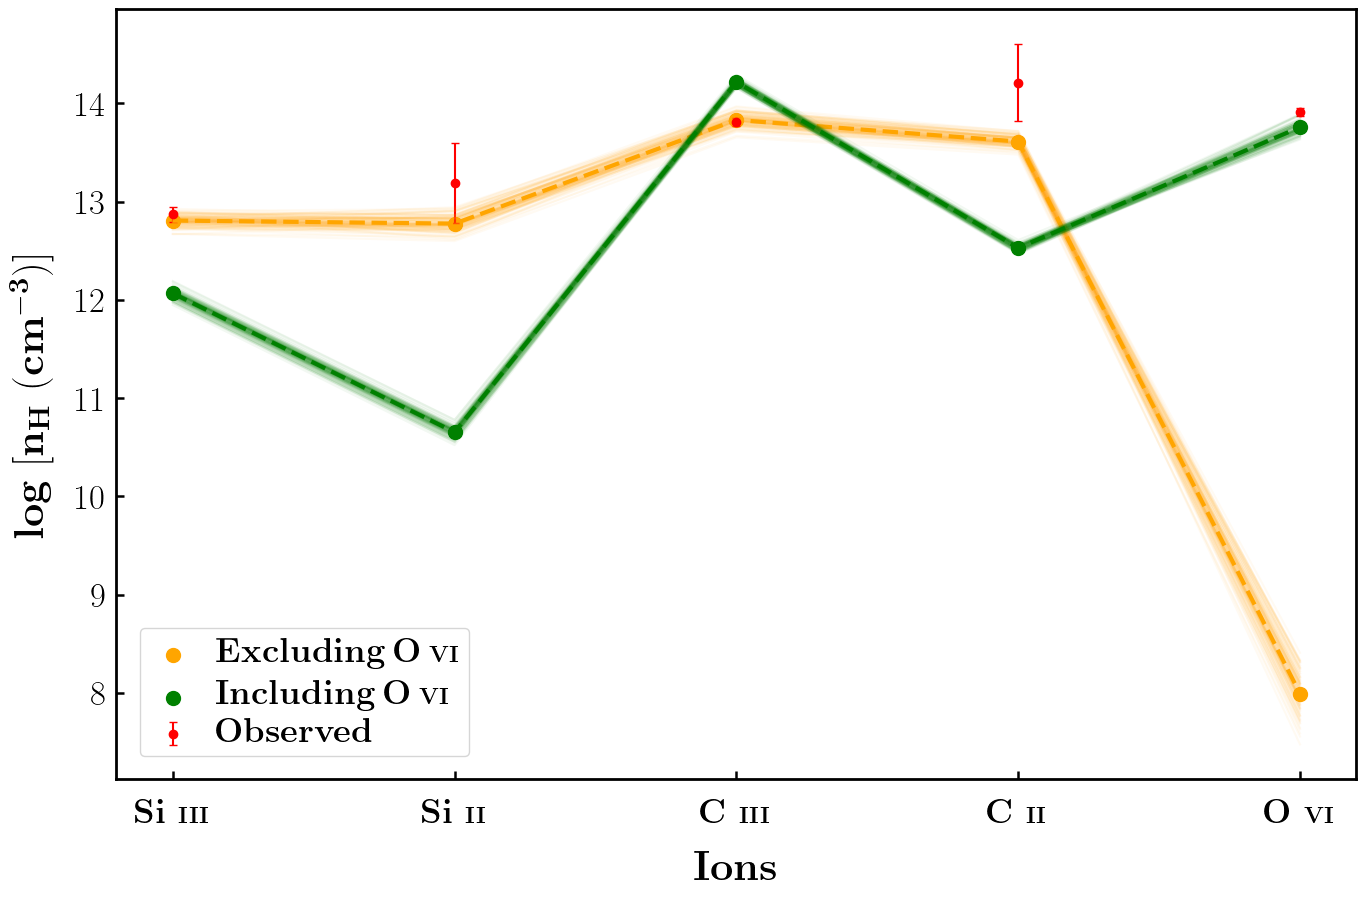
\includegraphics[width=\columnwidth]{Figures/Observed-and-predicted.png}
\caption{Modelled and observed column densities for the component III based on photoionization modelling. Red error bars shows the observed column densities and corresponding 1-$\sigma$ errors in column densities. The green and orange filled circles are the modelled column densities for the including \ion{O}{vi} and excluding \ion{O}{vi} case of PIE modelling. And the light green and light orange lines are modelled column densities with densities and metallicity sampled from normal distributions of log $n_H$ and log Z of including \ion{O}{vi} and excluding \ion{O}{vi} case respectively.}
\label{fig:obs_predicted}
\end{figure} 

As the above solution couldn't fit the observations well, we consider another case where all ions other than \ion{O}{vi} are arising from same gas phase. So, now we calculate the $\chi^2$ from column densities of other ions than \ion{O}{vi} and then minimise this $\chi^2$ to fit the model. This solution gives a good fit for the observed column densities of all the ions but now the \ion{O}{vi} is under-produced by orders of magnitude as seen in figure \ref{fig:obs_predicted} (orange filled circles) . This solution gives a temperature of about $1.0 \times 10^4$ K. This solution predicts a total Hydrogen column density, $\text{log [N(H)} \ \text{cm}^{-2}]$ = 17.92, smaller by nearly 2 orders than the previous case and a higher density, log $n_H \ (\text{cm}^{-3})$ = -2.24. This gives a line of sight thickness for the cloud to be around 50 pc.
As this case gives a better fit, we consider this to be the more correct description of the physical conditions in the absorber and draw our inferences based on this solution.

The log $n_H$, log Z and $\chi^2$ values for both the cases are given in table \ref{tab:compIII_PIE_sol}. And the physical properties of all the three components are listed in table \ref{tab:physical_param} based on the ionization modelling used.

\begin{table}[!htbp]
\centering
\begin{tabular}{cccc}
        \hline \hline
       \head{Case} & \head{log $\mathbf{n_H \ (\text{cm}^{-3})}$} & \head{log Z/$\mathbf{\text{Z}_{\odot}}$} & \head{$\mathbf{\chi^2}$}
       \tabularnewline \hline  
      All ions                  &  -3.88 $\pm$ 0.02    & -1.51 $\pm$ 0.03   &  275.67  \tabularnewline 
      Excluding \ion{O}{vi}     &  -2.24 $\pm$ 0.03    & -0.31 $\pm$ 0.06   &  4.27    \tabularnewline
     \hline \hline \tabularnewline
    \end{tabular}
\caption{Cloudy modelling solutions for absorber at z $\sim$ 0.34790. In case of all ions $\chi^2$ is calculated using the column densities of all the ions but for excluding \ion{O}{vi} ion case, $\chi^2$ is calculated by excluding \ion{O}{vi} column density so as to show that this fits other ions very well.}
\label{tab:compIII_PIE_sol}
\end{table}

\begin{landscape}
\thispagestyle{empty}
    
\begin{table}[!p]
\centering
\hspace*{-41mm}
\captionsetup{oneside,margin={0cm,15mm}}
\begin{tabular}{cccccccccc}
        \hline \hline \tabularnewline
        
      \head{Absorber}   & \head{Ions} & \head{log N({\text{H\,\small{\textsc{\uppercase{i}}}}})} & \head{Model}  & \head{log N(H)} & \head{log n\textsubscript{H}} & \head{log Z/$\mathbf{\text{Z}_{\odot}}$} & \head{Size} & \head{T} & \head{P/K} \\ \tabularnewline 
      \head{}   & \head{} & \head{$\mathbf{({cm}^{-2})}$} & \head{}  & \head{$\mathbf{({cm}^{-2})}$} & \head{$\mathbf{({cm}^{-3})}$} & \head{} & \head{(kpc)} & \head{(K)} & \head{$\mathbf{({cm}^{-3} \ K)}$} \\ \tabularnewline
      \hline \tabularnewline

z $\sim$ 0.34678                  &      \ion{H}{i}                          &  13.46                 &  -  &    -    &   -   &  -    &  -    &  $\leq \ 8.7 \times 10^4$  & -  \\ \tabularnewline

\multirow{2}{*}{z $\sim$ 0.34758} & \multirow{2}{*}{\ion{H}{i}, \ion{O}{vi}} & \multirow{2}{*}{14.13} & PIE &  18.45  & -4.51 & -0.31 & 29.47  & $2.5 \times 10^4$   & 0.77  \\
                                  &                                          &                        & Hybrid & $\lesssim$ 19.62  &  $\gtrsim$ -3   & $\gtrsim$ -0.4  & $\lesssim$ 13.35  & $1.9 \times 10^5$   & $\gtrsim $ 194.98  \\ \tabularnewline
                                  
\multirow{2}{*}{z $\sim$ 0.34790} & \multirow{2}{*}{\ion{H}{i}, \ion{O}{vi}, \ion{C}{ii}, \ion{C}{iii}, \ion{Si}{ii}, \ion{Si}{iii}} & \multirow{2}{*}{16.10} & PIE (All ions) &  19.87 & -3.88 & -1.51 & 180.75 & $2.8 \times 10^4$ & 3.68 \\
                   &                    &                    & PIE (Excluding \ion{O}{vi}) &  17.92 & -2.24 & -0.31 & 0.05 & $1.0 \times 10^4$ & 59.02 \\ 

        \tabularnewline \hline \hline \tabularnewline
    \end{tabular}
\caption{Physical properties of the absorbers based on Voigt profile measurement and CLOUDY ionisation modelling. The PIE solution for absorber at z $\sim$ 0.34758 is based on the excluding \ion{O}{vi} case PIE solution of the absorber at z $\sim$ 0.34790.}
\label{tab:physical_param}
\end{table}

\end{landscape}



\section{Origin of {\text{O\,\small{\textsc{\uppercase{vi}}}}} in the Absorber}


\subsection{Component II} \label{sec:temp_calc_b}

The large \emph{b} value indicates a large value of the temperature. As we the \ion{O}{vi} absorption is coincident with the BLA we can directly estimate this temperature using their \emph{b} values. The \emph{b} values which we get from Voigt profile have both thermal and non thermal contributions. 
\begin{equation} \label{eq:b_HI}
\emph{b}(\ion{H}{i})=\sqrt{{{\emph{b}^2}_{\text{thermal}}(\ion{H}{i})}+{{\emph{b}^2}_{\text{non-thermal}}}}
\end{equation}
\begin{equation}
\emph{b}(\ion{O}{vi})=\sqrt{{{\emph{b}^2}_{\text{thermal}}(\ion{O}{vi})}+{{\emph{b}^2}_{\text{non-thermal}}}}
\end{equation}
\begin{equation} \label{eq:b_thermal}
\emph{b}_{\text{thermal}}=\sqrt{\frac{2kT}{m}}
\end{equation}
Where, $k, \ T \text{and} \ m$ are Boltzmann constant, temperature and atomic mass of the species respectively.
\\\\
From equation \ref{eq:b_thermal} we have,
\begin{equation}
{\emph{b}}_{\text{thermal}}(\ion{H}{i})=4\ {\emph{b}}_{\text{thermal}}(\ion{O}{vi})
\end{equation}
Solving above equations for T gives, $T={10}^{{5.29}_{-0.08}^{+0.07}}$ K, which lies in the temperature range of WHIM. This temperature results in ${\emph{b}}_{\text{thermal}}$(\ion{H}{i}) $\sim 57 \ \text{km} \  \text{s}^{-1}$ and ${\emph{b}}_{\text{thermal}}$(\ion{O}{vi}) $\sim 14 \ \text{km} \  \text{s}^{-1}$. High temperature contributes to around 91 \% of the broadening of the \ion{H}{i} line whereas the \ion{O}{vi} line broadening is dominated by non-thermal components. An inherent assumption in this calculation is that the both lines have same contributions from non-thermal components. 

The ionization fraction of \ion{O}{vi} in collisional ionization equilibrium peaks around $10^{5.7}$ K. We are getting a nearby temperature of ${10}^{5.29}$ K, so the \ion{O}{vi} could be tracing a collisionally ionised gas phase. 

\subsection{Component III}

As discussed in section \ref{sec:compIII_PIE}, we consider two cases of photoionization models, one solution is able to explain \ion{O}{vi} column density but can't model column densities of other ions. Another solution models the column densities of other ions but fails to explain the \ion{O}{vi} column density. We discard the first case on grounds of poor fit and large line of sight length. And accept the second case to be more accurate description of the absorbing cloud conditions. We argue that as the other ions excluding \ion{O}{vi} can be explained by photoionisation models, they must be arising from a cool photoionised gas phase. But the question still remains that from where the \ion{O}{vi} absorption is coming from ?  

There have been similar instances in literature where the \ion{O}{vi} can't be explained from photoionised phase and could possibly be tracing a warm phase \citep[see e.g.][]{Pradeep-2020,Anshul-2021}. So,
we assert that \ion{O}{vi} absorption may be arising from a different hidden phase in the absorber and possibly tracing a collisionally ionised phase. However, to infer about this 'hidden' phase we need details on the associated Lyman $\alpha$ component. Since the Lyman $\alpha$ feature in absorber system is almost saturated with 3 components, we can't get any insights on the contributions from the hidden $\text{4}^{\text{th}}$ component if there is any.

\section{Galaxy environment of the absorber}

Galaxies, galaxy groups or clusters can have large gaseous halos surrounding them, called the circumgalactic medium (CGM) extending upto kpc scales. Our absorber system could be tracing one such halo. So we lookout for the galaxies around the absorber to check if this is the case. We search galaxies with velocity separations within 1000 km $\text{s}^{-1}$ from the absorber and within 15$\arcmin$ on the plane of sky from the quasar line of sight, which spans around 4.4 Mpc at the absorber redshift \footnote{Assuming a flat $\Lambda$CDM cosmology with $\text{H}=69.6 \ \text{km} \ \text{s}^{-1} \ \text{Mpc}^{-1}$}. No spectroscopically identified galaxies were found in the SDSS DR17 \citep{SDSS_DR17} footprints with above constraints.  SDSS' 90 per cent spectroscopic completeness limit of r < 17.8 \citep{strauss_SDSS} gives luminosity limit of L $\gtrsim$ 2.77 $\text{L}^{*}$ at z $\sim$ 0.347 assuming luminosity functions calculated by \citet{ilbert_GLF}. This implies that the SDSS spectroscopic survey has only sampled the bright galaxies only. So there could be sub-$\text{L}^{*}$ galaxies present around the absorber system

Our line of sight was also observed under the VIMOS survey \citep{vimos_data} (PI - Thomas Shanks, Program Id : 097.A-0535(D)). The VIMOS field of view in imaging mode comprises of 4 quadrants. The quasar PG0003+158 was centered in the $\text{3}^\text{rd}$ quadrant out of this 4 quadrants. The field was observed in B (383-478 nm) and R (579-713) filters.

\begin{table}[!t]
\centering
    \begin{tabular}{cccccccc}
        \hline \hline
       \head{R.A.} & \head{Dec.} & \head{z} & \head{$\mathbf{\Delta v}$} & \head{$\mathbf{\eta}$} & \head{$\mathbf{\rho}$}  & \head{r} & \head{L} \\ 
        &  &  & \head{$\mathbf{(\text{km \ s}^{-1})}$} & \head{(arcmin)} & \head{(Mpc)}  &  & \head{($\mathbf{L^*}$)}
       \tabularnewline \hline  \tabularnewline
        1.43341  &  15.97131  &  0.3351  &  -2564  &  12.1  &  3.6  &  20.387   &  0.24   \\
        1.52570  &  15.98456  &  0.3466  &  -200  &  10.9  &  3.2  &  21.719   &  0.07  \\
        1.48286  &  16.14235  &  0.3517  &  838  &  1.5  &  0.4   &  21.533   &  0.09  \\
        1.43069  &  16.16771  &  0.3582  &  2153  &  3.8  &  1.1  &  19.342   &  0.72  \\
        1.44071  &  16.16933  &  0.3593  &  2374  &  3.3  &  1.0  &  19.745   &  0.50  \\
       \tabularnewline \hline \hline 
    \end{tabular}
\caption{Galaxies in the neighbourhood of the absorber system identified in VIMOS survey. Velocity is taken to be zero at z = 0.347586}
\label{tab:galaxies}
\end{table}

5 galaxies were identified within the field. We looked for these galaxies in the SDSS photometric survey and found all of the 5 galaxies providing us with the photometric data. The details of the galaxies are given in table \ref{tab:galaxies}. The table gives the position, redshift, velocity separation, separation on the plane of sky ($\eta$) , projected distance on the plane of sky ($\rho$) and the SDSS r-band magnitude and luminosity of the galaxies. Two of the galaxies were within 1000 km $\text{s}^{-1}$ and 15$\arcmin$ from the quasar line of sight. Figure \ref{fig:galaxy} shows the galaxies around the absorber system color coded with the absolute velocity separation from the absorber system (z=0.347586). The cross mark in the center is the line of sight of PG 0003+158. The blue and orange dashed curves show the projected distance at the absorber redshift (z=0.347586) of 500 kpc and 1 Mpc respectively. There is one galaxy within a projected separation of 500 kpc but it separated by around 838 km $\text{s}^{-1}$ from the absorber. We find one galaxy at 200 km $\text{s}^{-1}$ from the absorber but it is at a projected distance of around 3.2 Mpc from the line of sight. 

\begin{figure}[!t]
% \vspace{-40mm}
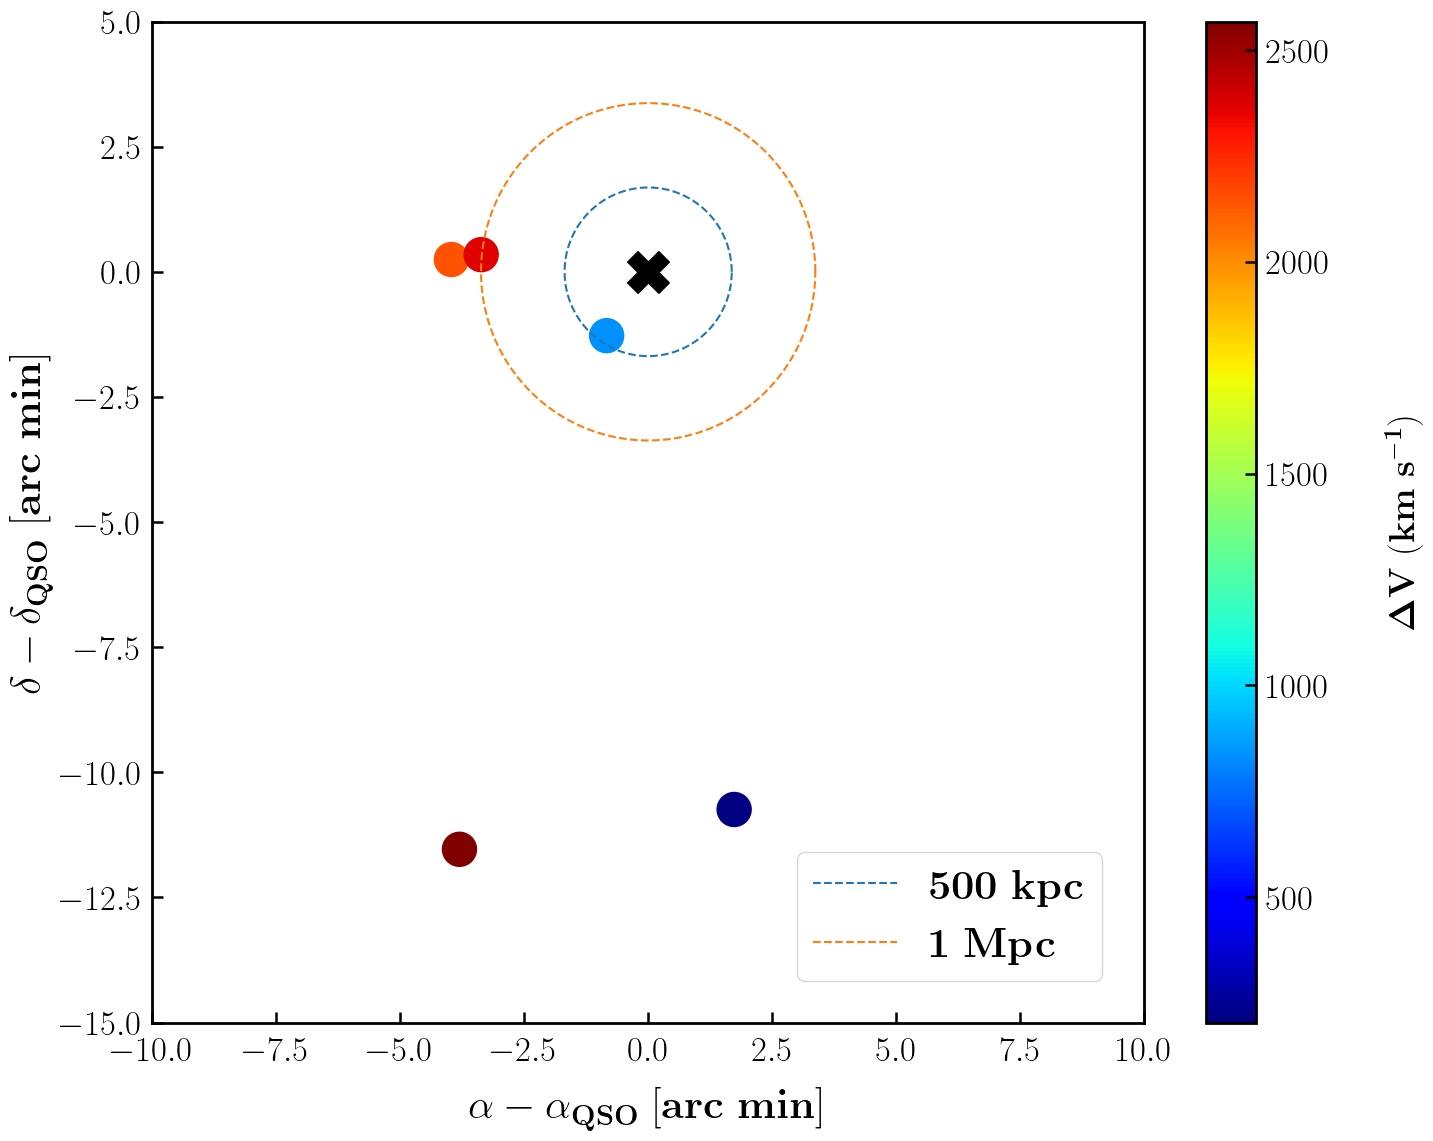
\includegraphics[width=\columnwidth]{Figures/galaxy_environment.png}
\caption{Galaxies around the absorber color-coded with their velocity separation from the absorber.}
\label{fig:galaxy}
\end{figure}

\citet{Prochaska-2011} gives the following scaling relation between luminosity and virial radius of a galaxy but warns that this is based on crude estimates and should serve as a mere guideline:

$$r_{vir}=r^{*}_{vir}\left(\frac{L}{L^{*}}\right)^{\beta}$$

with $r^{*}_{vir}=250$ kpc and $\beta=0.2$. For the galaxy at projected distance of 0.4 Mpc which is the closest in projected distance, $r_{vir}$ comes out to be 155 kpc which is 2.6 times less than the projected distance. So the absorber is quite far from the CGM of this galaxy. The virial radii of other galaxies are also not large enough.

We see that the absorber lies in a galaxy under-dense region, so the absorber could be tracing a large scale filamentary structure in the cosmic web or CGM of a faint galaxy with a luminosity less than 0.07 L$^*$ which is not sampled in the current observations.




\chapter{Hunt for BLAs : The Survey} \label{ch:Survey}

The foremost goal of the current study is to do a survey of BLAs over a large data-set and then estimate their contribution in the closure density of $\Omega_b$. In this chapter we describe our approach to carry out this exhaustive survey.

\section{Shortlisting the BLA candidates} \label{sec:BLA-candidates}

\citet{danforth-2016} have identified a total of 2611 absorber systems in their study of low redshift intergalactic medium. We need to find suitable candidates for our survey of BLAs from these 2611 absorbers.

We use two criterias to select BLA candidates for our survey. First, we look for broad Ly$\alpha$ lines in all the 2611 absorbers. For a Ly$\alpha$ line to be adjudged as `broad', we fix our threshold for \emph{b} value to be greater than 45 km s$^{-1}$ in the preliminary fitting done by \citet{danforth-2016}. Assuming a complete thermal broadening, $\emph{b}=45$ km s$^{-1}$ gives a temperature of $\approx 1.2 \times 10^5$ K, which lies in the lower ranges of the temperature of WHIM. By giving this constrain, we get 568 such systems in the complete data-set.

As discussed in section \ref{sec:WHIM-BLA}, multiple lines or contaminations from other lines can blend together to give rise to broad absorption features. In such cases, we need to carefully model these broad lines and confirm that these are actually tracing hot collisionally ionised gas phase so that they are indeed probing WHIM and not just cool photoionised phase. We need to perform ionisation modelling for it. To model the ionisation conditions of the absorber systems, we need metal ion column densities. So we search for systems showing metal line absorption in these 568 `broad' systems. We need at least three distinct metal ions (not lines) to better constrain the ionisation state of an absorber system. This sets our second criteria that there should be minimum of three metal ion absorption in the absorber systems. Upon putting this constrain, we get 29 systems having at least 3 distinct metal ions out of 568 already identified systems. Out of these 29 systems, we have already studied one of the absorber in chapter \ref{ch:PG0003}. Table \ref{tab:BLA-candidates} lists the lines of sight, redshift of the absorber and the ions detected in the systems these 29 identified BLA candidate absorber systems. Figure \ref{fig:metal-ions-hist} shows the distribution of different metal ions found in these 29 absorber systems. 


\begin{figure}
    \centering
    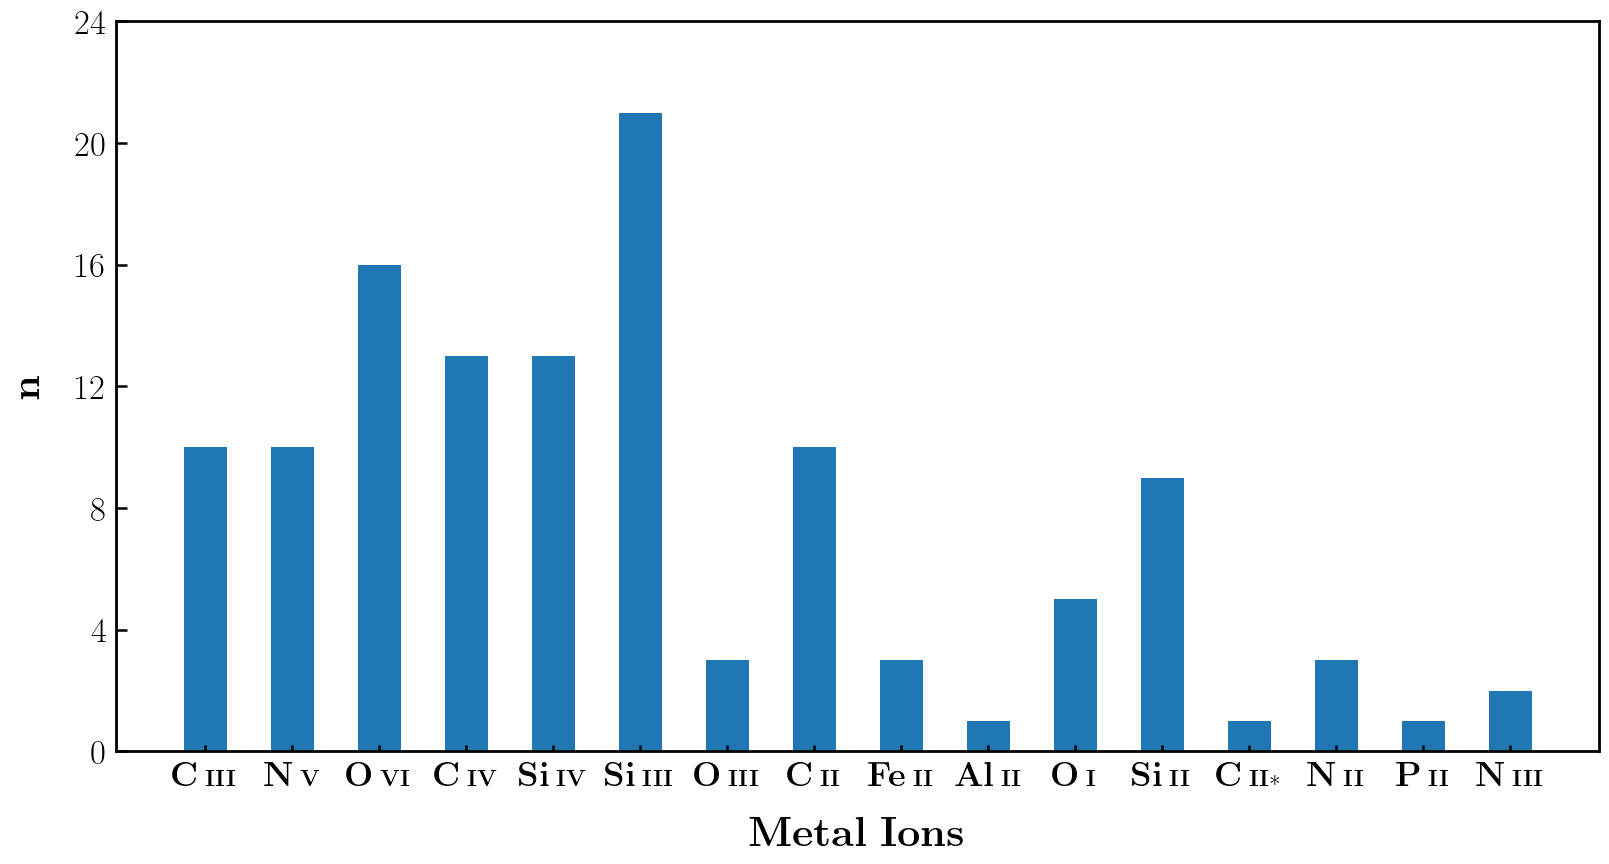
\includegraphics[width=\linewidth]{Figures/metal-ions.png}
    \caption{No. of different metal ions in all the 29 absorber systems.}
    \label{fig:metal-ions-hist}
\end{figure}


\begin{table}
\centering
\vspace{5mm}
\hspace*{-15mm}
    \begin{tabular}{cccc}
        \hline \hline
       \head{S. no.} & \head{Line of Sight} & \head{$\mathbf{z_{abs}}$} &  \head{Metal ions}
       \tabularnewline \hline  \tabularnewline
1    &    1ES1553+113   &   0.187731   &  \ion{C}{iii}, \ion{O}{vi}, \ion{N}{v}   \\ 
2    &    3C263   &   0.063275   &  \ion{C}{iv}, \ion{Si}{iii}, \ion{Si}{iv}   \\ 
3    &    3C263   &   0.140754   &  \ion{C}{iv}, \ion{Si}{iii}, \ion{O}{vi}   \\ 
4    &    3C57   &   0.077493   &  \ion{C}{iv}, \ion{Si}{iv}, \ion{N}{v}   \\ 
5    &    H1821+643   &   0.170062   &  \ion{Si}{iii}, \ion{O}{vi}, \ion{N}{v}   \\ 
6    &    H1821+643   &   0.224832   &  \ion{Si}{iii}, \ion{O}{vi}, \ion{C}{iii}   \\ 
7    &    HE0056-3622   &   0.043318   &  \ion{C}{iv}, \ion{Si}{iii}, \ion{N}{v}   \\ 
8    &    PMNJ1103-2329   &   0.003975   &  \ion{C}{iv}, \ion{Si}{iii}, \ion{Si}{iv}, \ion{N}{v}   \\ 
9    &    PG0003+158   &   0.386094   &  \ion{C}{iii}, \ion{O}{vi}, \ion{O}{iii}, \ion{N}{v}   \\ 
10    &    PG0003+158   &   0.347586   &  \ion{C}{ii}, \ion{C}{iii}, \ion{Si}{ii}, \ion{Si}{iii}, \ion{O}{vi}\\ 
11    &    PG0003+158   &   0.421880   &  \ion{O}{vi}, \ion{O}{iii}, \ion{C}{iii}   \\ 
12    &    PG0832+251   &   0.017520   &  \ion{C}{iv}, \ion{Si}{iv}, \ion{C}{ii*}, \ion{O}{i}, \ion{Si}{iii}, \ion{C}{ii}, \ion{Si}{ii}, \ion{Fe}{ii}, \ion{Al}{ii}, \ion{N}{v}   \\ 
13    &    PG1116+215   &   0.138527   &  \ion{C}{iv}, \ion{Si}{iv}, \ion{N}{ii}, \ion{P}{ii}, \ion{Si}{iii}, \ion{Si}{ii}, \ion{C}{ii}, \ion{O}{vi}, \ion{N}{v}   \\ 
14    &    PG1121+422   &   0.192434   &  \ion{Si}{iv}, \ion{C}{iii}, \ion{Si}{iii}, \ion{Si}{ii}, \ion{C}{ii}, \ion{O}{vi}   \\ 
15    &    PG1216+069   &   0.006390   &  \ion{O}{i}, \ion{Si}{ii}, \ion{C}{ii}   \\ 
16    &    PG1216+069   &   0.282195   &  \ion{Si}{iii}, \ion{O}{vi}, \ion{C}{iii}   \\ 
17    &    PG1222+216   &   0.054491   &  \ion{C}{iv}, \ion{Si}{iii}, \ion{Si}{iv}   \\ 
18    &    PG1222+216   &   0.378600   &  \ion{Si}{iii}, \ion{O}{vi}, \ion{O}{iii}, \ion{C}{iii}   \\ 
19    &    PG1259+593   &   0.046107   &  \ion{C}{iv}, \ion{Si}{iii}, \ion{Si}{iv}   \\ 
20    &    PG1424+240   &   0.146789   &  \ion{C}{iv}, \ion{Si}{iii}, \ion{O}{vi}, \ion{Si}{iv}   \\ 
21    &    PHL1811   &   0.080837   &  \ion{C}{iv}, \ion{Si}{iv}, \ion{N}{ii}, \ion{O}{i}, \ion{Fe}{ii}, \ion{Si}{ii}, \ion{C}{ii}   \\ 
22    &    PKS0405-123   &   0.167125   &  \ion{Si}{iv}, \ion{N}{ii}, \ion{C}{iii}, \ion{O}{i}, \ion{Si}{iii}, \ion{Si}{ii}, \ion{C}{ii}, \ion{O}{vi}, \ion{N}{iii}, \ion{N}{v}   \\ 
23    &    PKS0637-752   &   0.161068   &  \ion{Si}{iii}, \ion{O}{vi}, \ion{N}{v}   \\  
24    &    PKS0637-752   &   0.417573   &  \ion{Si}{iii}, \ion{O}{vi}, \ion{C}{iii}   \\ 
25    &    PKS1302-102   &   0.094864   &  \ion{Si}{iii}, \ion{Si}{ii}, \ion{C}{ii}   \\ 
26    &    RXJ0439.6-5311   &   0.005602   &  \ion{C}{iv}, \ion{Si}{iii}, \ion{Si}{iv}   \\ 
27    &    J135712.61+170444   &   0.097767   &  \ion{C}{iv}, \ion{Si}{iv}, \ion{Si}{iii}, \ion{C}{ii}, \ion{O}{vi}   \\ 
28    &    SBS1108+560   &   0.463201   &  \ion{C}{iii}, \ion{O}{i}, \ion{Si}{iii}, \ion{Si}{ii}, \ion{C}{ii}, \ion{O}{vi}, \ion{N}{iii}   \\ 
29    &    UKS0242-724   &   0.063775   &  \ion{Fe}{ii}, \ion{Si}{ii}, \ion{C}{ii}   \\  
       \tabularnewline \hline \hline 
    \end{tabular}
\caption{Details of the 29 BLA candidate absorber system shortlisted  for the survey.}
\label{tab:BLA-candidates}
\end{table}


\section{Survey methodology}

We have identified 28 additional BLA candidate systems for our survey. We need to do the Voigt profile fitting to the absorption lines identified in these systems. These will give us the column densities and Doppler parameters of the ions in the system and also their redshifts (velocities). We will further use these quantities to model the ionisation conditions in these absorber systems. 

The distribution of these quantities can give valuable insights towards our understanding of the intergalactic medium and the baryon content within IGM. As discussed in chapter \ref{chap:intro}, that \ion{O}{vi} is good tracer of WHIM. \ion{O}{vi} absorption is seen in 16 out of these remaining 16 absorbers. For the remaining 12 candidates, \ion{O}{vi} is not a non-detection. The \ion{O}{vi} 1032, 1038 lines fall out the coverage of the HST/COS FUV channel at redshifts below $\sim 0.093854$ and all these remaining 12 systems are at redshift below 0.093854. So \ion{O}{vi} is not covered in these systems. However, for one system which is along the LOS of PKS1302-102 at $z_{abs}=0.094864$, the \ion{O}{vi} 1038 line was just falling just on the edge of the spectrum where both S/N and sensitivity both low. So, \ion{O}{vi} absorption was not considered for this system. 

We first model the ionisation conditions in the 16 \ion{O}{vi} absorbers and see if we can explain the origin of \ion{O}{vi} through photoionisation models using the similar method used for the absorber in chapter \ref{ch:PG0003}. For, the remaining 12 non-\ion{O}{vi} absorber, we model the ionisation conditions based on the ions detected to estimate the density and metallicity in these systems. 

Then, we will use the results from this survey to estimate the baryon content in BLAs and their contribution to cosmic closure density, $\Omega_b$, the details of which are described in the upcoming chapter.

The Voigt profile fitting and ionisation modelling results are given in appendix \ref{app:survey-results} after the references.


\section{Survey statistics}

\subsection{Voigt profile fitting}

This survey of 28 absorbers spanned 22 lines of sight. These 22 lines of sight have total \ion{H}{i} (Lyman-$\alpha$) redshift pathlength of $\Delta z = 5.561$. A total of 413 absorption lines were identified and fitted with Voigt profiles. These 413 lines shown absorption from 15 different metal ions apart from \ion{H}{i} absorption.  


\begin{figure}
    \centering
    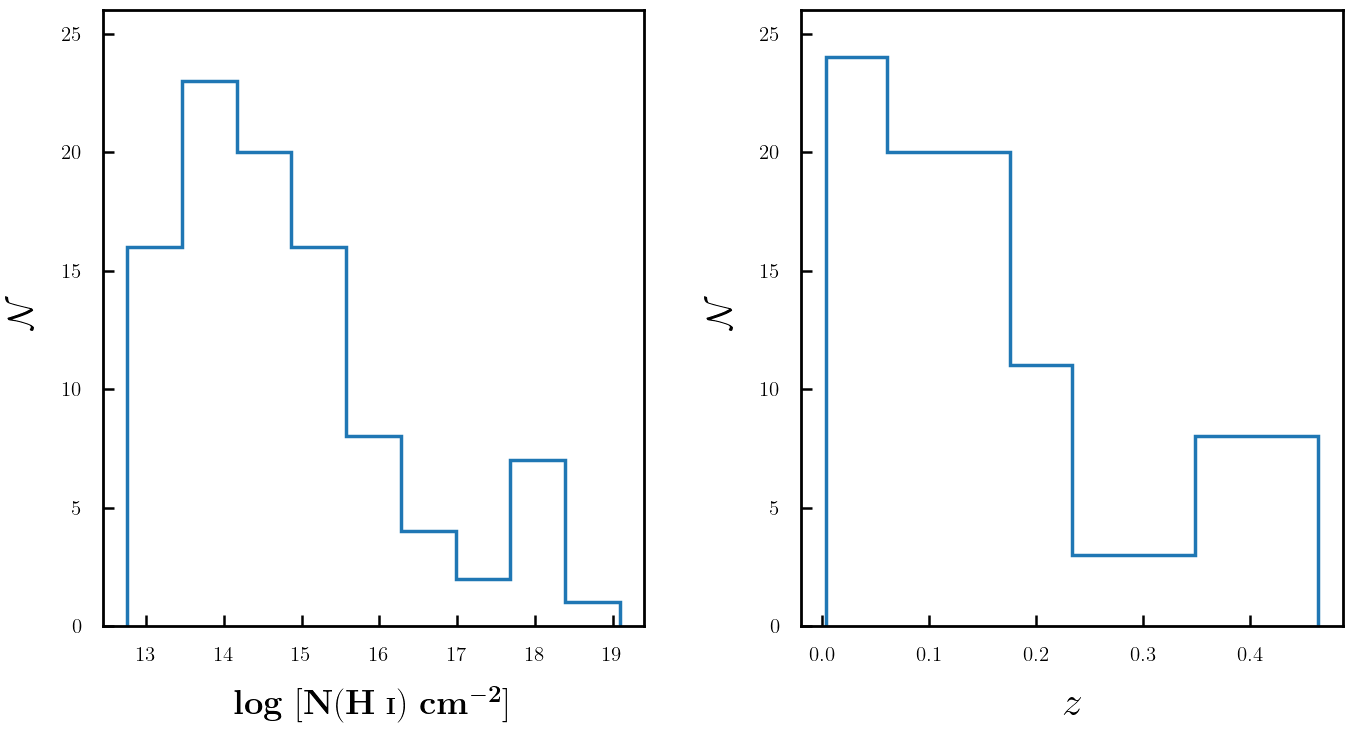
\includegraphics[width=\linewidth]{Figures/HI_distribution_survey.png}
    \caption{Left panel - distribution of \ion{H}{i} column densities, Right panel - distribution of redshift of \ion{H}{i} components}
    \label{fig:HI_distribution}
\end{figure}

\subsection{Ionisation modelling}





\section{Survey so far} \label{sec:OVI-BLA}

Out of the 28 BLA candidate systems identified as described in section \ref{sec:BLA-candidates}, we first focus on a subset of these systems which have \ion{O}{vi} absorption, as \ion{O}{vi} is a good tracer of WHIM. We have 16 such absorber systems. We begin the survey with these 16 systems. First step of the survey is to fit the Voigt profiles to all the lines identified in these systems. Currently, we have completed the preliminary fitting of these 16 absorber systems. The system plots of all these 16 systems are given in appendix \ref{ap:system-plots}.


\chapter{Estimating $\Omega_\text{b}(\text{BLA})$} \label{ch:Omega-b}

In this chapter we discuss the estimation of the baryon energy density trapped in BLAs, i.e. $\Omega_\text{b}(\text{BLA})$, using our BLA survey which is the cornerstone of the current work. We will statistically estimate the $\Omega_\text{b}(\text{BLA})$ from our survey results. And then we will determine how much BLAs contribute to the baryon budget ($\Omega_\text{b}$) of the current universe.

\section{Methodology to determine $\Omega_\text{b}(\text{BLA})$}

The baryon content of any ion in terms of the current critical density $(\rho_{cr})$ of the universe can be estimated by integrating over the bivariate frequency distribution of the absorbers as function of column density and redshift of that ion and is given as :

\begin{equation} \label{eqn:omega_ion}
    \Omega_{\text{ion}} = \frac{H_0 m_{\text{ion}}}{c \rho_{\text{cr}}} \int \frac{\partial ^2 \mathcal{N}}{\partial N \partial X} N dN 
\end{equation}

\vspace*{3mm}

Where, $H_0$ is the current value of Hubble's constant, \\ \hspace*{19mm}
$m_\text{ion}$ is the the mass of ion, \\ \hspace*{19mm}
$c$ is the speed of light in vacuum, \\ \hspace*{19mm}
$\mathcal{N}$ is the number of absorbers at column density $N$ and path length $X$

\newpage

The path length $X$ is function of redshift (\emph{z}) and denotes the total absorption path length available for absorption. A non-evolving population of absorbers will show an invariant number density per unit absorption pathlength \citep{Becker-2011}. It is defined as :

\begin{equation}
    X(z)=\int_0^z  (1+z')^2 \frac{H_0}{H(z')} dz'
\end{equation}

Now, assuming a flat $\Lambda \text{CDM}$ cosmology, we can write the Hubble's constant at any \emph{z} as :

\begin{equation}
    H(z) = H_0 \left[\Omega_m(1+z)^3+\Omega_\Lambda\right]^{1/2}
\end{equation}

with $\Omega_m=0.31$ and $\Omega_\Lambda=0.69$ (ref). This gives,

\begin{equation}
    X(z)=\int_0^z  \frac{(1+z')^2}{\left[\Omega_m(1+z')^3+\Omega_\Lambda\right]^{1/2}} dz'
\end{equation}

However, whole pathlength of X may not be available for absorption due to the presence of Ly$\alpha$ forest lines, absorption from strong ISM lines and intervening IGM lines also in the spectrum. So, some correction needs to be made to get the unblocked absorption pathlength. To calculate this correction, we have developed an interactive program, where we manually select the wavelength regions showing strong absorption features from the above mentioned lines along each sight line. So we exclude these wavelength regions to calculate the unblocked absorption pathlength.

Now, to get the baryon content of BLAs using equation \ref{eqn:omega_ion}, we can use total Hydrogen column density, N(H), and $m_{ion}=\mu . m_H$, where $\mu$ is the mean atomic mass in a.m.u. and $m_H$ is the mass of Hydrogen atom. We take $\mu=1.32$ for $\text{Y}_\text{He}=0.2446$ \citep{Peimbert-2016} taking in account the Helium abundance in the universe. But N(H) is not a directly observable quantity, instead we can get neutral Hydrogen column density, N(\ion{H}{i}), from observations. So we need the correct for the ionisation of Hydrogen to get N(H) from observable N(\ion{H}{i}). This ionisation correction is not trivial and require number of assumptions.

If the gas is collisionally ionised, then we can estimate the hydrogen ionization fraction, which is the ratio of amount of total hydrogen and neutral hydrogen, in equilibrium using the models given by \citet{Sutherland-1993} which related the ionisation fraction to the temperature of the gas. It gives following relation :

\begin{equation} 
    \log f_H \approx 5.4 \log T - 0.33(\log T)^2 -13.9
\end{equation}

This relation is valid in the temperature regimes of $10^5-10^7$ K. Figure \ref{fig:fH} shows the variation of $f_H$ with $T$ based on above relation . We can use this to convert N(\ion{H}{i}) to N(H). However, we need to note that at densities lower than $n_H < 10^{-5} \ \text{cm}^{-3}$, photoionisation from UV background could result in higher hydrogen ionization fraction. But since we don't have the hydrogen densities in the absorbers, so we could possibly underestimate the $f_H$ in such cases (see \citet{Richter_2020, Fang-2001} for more details). Still, we need the temperature to get the ionisation correction. We could only estimate the temperature where the BLA is aligned with some other ion like \ion{O}{vi}. We have only few such cases. In rest of the cases, where we don't have an estimate of temperature, we use the Doppler width, \emph{b}, of the BLA to estimate the temperature assuming pure thermal broadening. This gives us an upper limit on the temperature of the absorber. Now, $b^2=2kT/m_H$, so $T=(m_H / 2k) b^2 $. 

\begin{figure}
    \centering
    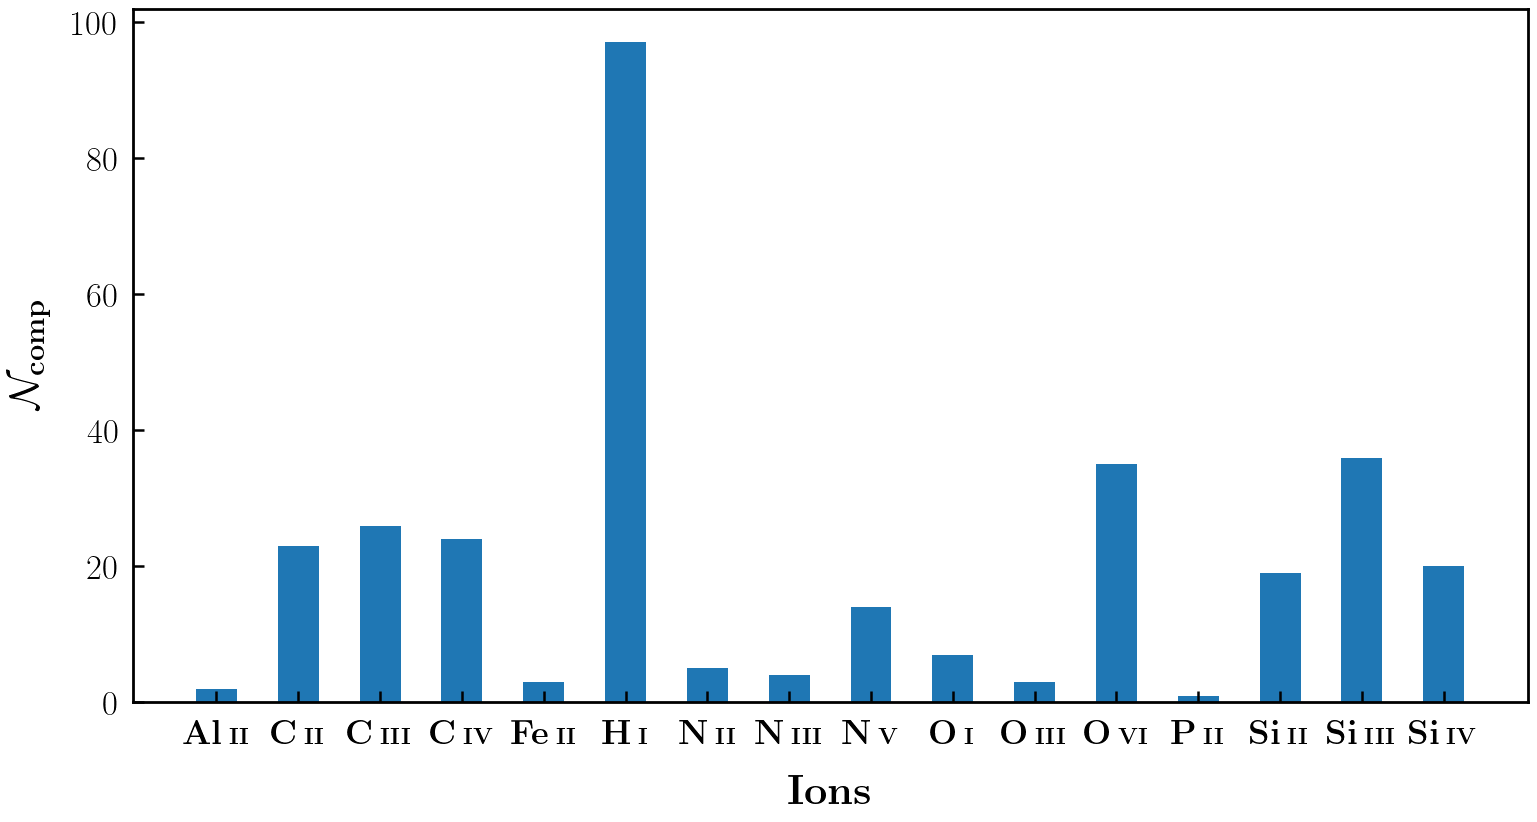
\includegraphics[width=\linewidth]{Figures/ion-component.png}
    \caption{Hydrogen ionisation fraction as a function of temperature.}
    \label{fig:fH}
\end{figure}

Now, as the neutral fraction of hydrogen is very low at the temperatures in WHIM, we can write :

\begin{equation*}
     \log f_H = \log \left(\frac{\ion{H}{i}+\ion{H}{ii}}{\ion{H}{i}}\right) \approx \log \left(\frac{\ion{H}{ii}}{\ion{H}{i}}\right)  \Rightarrow  \ion{H}{ii}= f_H \ion{H}{i}
\end{equation*}

\begin{equation*}
     \Rightarrow  N(\text{H}) = N(\ion{H}{i})+N(\ion{H}{ii}) = (1+f_H)N(\ion{H}{i}) \approx f_H N(\ion{H}{i})
\end{equation*}

Since don;t have the bivariate frequency distribution function, we approximate the intergral in equation \ref{eqn:omega_ion}, which is commonly done, as : 

\begin{equation} \label{eqn:int-approx}
    \int \frac{\partial ^2 \mathcal{N}}{\partial N  \partial X} N dN \simeq \frac{\sum N_{obs}}{\Delta X} 
\end{equation}

Where $N_{obs}$ is the observed column density of the ion and $\Delta X$ is the total unblocked pathlength available. Now using equation \ref{eqn:omega_ion}, the approximation in equation \ref{eqn:int-approx} and including ionisation correction we can estimate $\Omega_\text{b}(\text{BLA})$ as :

\begin{equation}
    \Omega_\text{b}(\text{BLA}) = \frac{H_0 \ \mu m_H}{c \rho_{\text{cr}}} \left. \sum_{i,j} f_{H_{i,j}} N(\ion{H}{i})_{i,j} \ \middle / \sum_j \Delta X_j \right.
\end{equation}

Where $j$ represents a line of sight and $i$ refers to the absorber along sight line $j$. So numerator is the sum over all the absorbers and the denominator is summed over all the lines of sight.  We use error propogation to find the uncertainity in the value of $\Omega_\text{b}(\text{BLA})$. We consider error in $f_H$, which depend on temperature, which inturn depend on the measured \emph{b} values and error in \ion{H}{i} column densities.  


 
 
\chapter{Conclusions and Future Work} \label{ch:conclusions}

\section{Conclusions}

The motivation for the current work comes from `the missing baryon problem' in the current universe. According, to which around 30\% of the baryons are missing from our observations in the current universe. Cosmological simulations show that these baryons could be residing in Warm Hot Intergalactic Medium at high temperatures ($10^5-10^7$) K and very low densities ($10^{-4} - 10^{-6} \ \text{cm}^{-3}$). This makes it difficult to detect WHIM, which has lead to uncertainties in the baryon census in this phase. In the current work we aim to address these uncertainties by surveying the broad Lyman-$\alpha$ absorbers (BLAs), which are thermally broadend to large Doppler widths above 40-45 km s$^{-1}$. But detecting broad features does not mean that we are always probing WHIM or high temperature gas phase. Broad features could also arise due to contaminations from other lines, line blending effects, poor S/N in the spectra. To ensure that the detected broad feature is indeed tracing WHIM and not other case mentioned above, we need to model the ionisation conditions in these absorber systems. If we find that the species in the absorbers are coming from collisionally ionised phase, then we could be sure that BLA candidate is tracing a warm-hot plasma as collisional ionisation is prominentatly seen at high temperatures. One such specie is \ion{O}{vi}, which is an excellent tracer of WHIM, as it's ionisation fraction in collisional ionisation peaks around temperatures of $\text{T} \sim 10^{5.7}$ K.   

We use high S/N HST/COS FUV observations for the current work. In the low redshift IGM survey done by \citet{danforth-2016}, they have studied 82 quasar sight lines, which have the highest quality available data. They have done the preliminary Voigt profile measurements on the absorption lines along these 82 sight lines. But we need more accurate Voigt profile measurements for our survey. So, we look for suitable candidates for our survey in their dataset. We shortlist systems which have \ion{H}{i} Doppler parameters above 45 km s$^{-1}$ in their preliminary measurements. Since we also need to model the ionisation conditions in these absorbers, which require metal ions. So we further put constrain that the absorbers should have absorption from atleast 3 distinct metal ions to model the ionisation conditions robustly. We find 29 absorber systems which satisfies these two constrains. These 29 systems are distributed along 22 different sight lines. The survey has a total unblocked \ion{H}{i} (Lyman-$\alpha$) redshift pathlength of $\Delta z = 5.561$.  We find a total of 37 BLA components in these systems. Out of the 29 absorbers, 17 systems show absorption from \ion{O}{vi}. We have identified a total 711 absorption lines in these 29 systems and have modelled the ionisation conditions in 39 components of these systems. In case of \ion{O}{vi} systems, we find that 20 out of 25 \ion{O}{vi} components could be tracing collisionally ionised gas phase and possibly probing warm-hot plasma. 

We make use of the results from this survey to estimate the baryon content in BLAs. We consider three sample of absorbers for this. First, we use absorbers where reliable estimate of temperature is available and ionisation modelling suggests collisional ionisation of \ion{O}{vi}, this gives us a very conservative lower limit on $\Omega_b(\text{BLA})$ to be $(1.8 \pm 0.5) \times 10^{-3} {h_{70}}^{-1}$. Our second sample considers absorbers where \ion{O}{vi} is found to be collisionally ionised. For this, we estimate the temperature from Doppler parameters assuming complete thermal broadening. This gives us $\Omega_b(\text{BLA})=(7.2 \pm 1.3) \times 10^{-3} {h_{70}}^{-1}$. The last sample includes all the BLA components found in our survey. This yields a very large value of $\Omega_b(\text{BLA})=(27.1 \pm 13.8) \times 10^{-3} {h_{70}}^{-1}$, which exceeds the prediction of baryon content in WHIM from cosmological simulations of around 50\%. We discuss the sources on uncertainties in these estimates. We finally compare these values with the total baryon energy density and find that BLAs can contribute around 15-20 \% to the total cosmic baryon budget in the current universe.

\section{Future work}

The future work includes incorporating more sight lines in the surevy to improve the statistics. We can extend the results from this survey to larger data set of general population of BLA systems to get the more robust estimate of the baryon content in these BLAs. Future studies could be also be aimed to explore the correlations between these BLAs and galaxies by doing systematic survey of galaxies around these absorber system. This can allow us to understand the origin of these absorbers. This would allow us to get insights on the metal enrichment of the IGM from the galaxies. This could also shed light on the various feedback processes happening in the circumgalactic medium of the galaxies, which play crucial rule in the formation and evolution of the galaxies.  




\bibliographystyle{mnras}
\bibliography{References}

\NoChapterHead

\Annexes{


\Annex{Sight lines shortlisted for survey} \label{ap:los}

This appendix gives the details of the 22 sight lines along which our 29 absorber systems lies.

\begin{table}
    \centering
    \hspace*{-20mm}
        \begin{tabular}{ccccccc}
            \hline \hline
           \head{S. no.} & \head{Sight line} & \head{R.A. (J2000)} &  \head{Dec. (J2000)} & \head{$\mathbf{z_{AGN}}$}  &  \head{Flux}\textsuperscript{a}  &  \head{AGN type}
           \tabularnewline \hline  \tabularnewline

            1  &  1ES 1553+113  &  15:55:43.04  &  +11:11:24.4  &  $>$0.4140  &  15.9  &  BLLac/FSRQ  \\
            2  &  3C 263  &  11:39:56.99  &  +65:47:49.2  &  0.6460  &  10.4  &  FR2/Sy1.2  \\
            3  &  3C 57  &  02:01:57.16  &  -11:32:33.1  &  0.6705  &  6.6  &  Sy1.2  \\
            4  &  H 1821+643  &  18:21:57.30  &  +64:20:36.0  &  0.2968  &  53.0  &  Sy1.2  \\
            5  &  HE 0056-3622  &  00:58:37.39  &  -36:06:05.0  &  0.1641  &  17.3  &  Sy1  \\
            6  &  PMN J1103-2329  &  11:03:37.60  &  -23:29:30.0  &  0.1860  &  2.1  &  BLLac/FSRQ  \\
            7  &  PG 0003+158  &  00:05:59.24  &  +16:09:49.0  &  0.4509  &  7.7  &  Sy1.2  \\
            8  &  PG 0832+251  &  08:35:35.80  &  +24:59:41.0  &  0.3298  &  3.5  &  QSO  \\
            9  &  PG 1116+215  &  11:19:08.60  &  +21:19:18.0  &  0.1763  &  45.7  &  Sy1.0  \\
            10  &  PG 1121+422  &  11:24:39.18  &  +42:01:45.0  &  0.2250  &  7.4  &  Sy1.0  \\
            11  &  PG 1216+069  &  12:19:20.93  &  +06:38:38.5  &  0.3313  &  12.3  &  NLSy1  \\
            12  &  PG 1222+216  &  12:24:54.45  &  +21:22:46.3  &  0.4320  &  17.0  &  Blazar  \\
            13  &  PG 1259+593  &  13:01:12.90  &  +59:02:07.0  &  0.4778  &  15.3  &  Sy1.0  \\
            14  &  PG 1424+240  &  14:27:00.39  &  +23:48:00.0  &  $>$0.6035  &  15.2  &  BLLac  \\
            15  &  PHL 1811  &  21:55:01.50  &  -09:22:25.0  &  0.1920  &  56.2  &  NLSy1  \\
            16  &  PKS 0405-123  &  04:07:48.43  &  -12:11:36.7  &  0.5740  &  32.1  &  Sy1.2  \\
            17  &  PKS 0637-752  &  06:35:46.50  &  -75:16:16.8  &  0.6500  &  8.0  &  FSRQ  \\
            18  &  PKS 1302-102  &  13:05:33.00  &  -10:33:19.0  &  0.2784  &  14.9  &  FSRQ/Sy1.2  \\
            19  &  RX J0439.6-5311  &  04:39:38.64  &  -53:11:31.6  &  0.2430  &  3.5  &  Sy1  \\
            20  &  SDSS J135712.61+170444  &  13:57:12.60  &  +17:04:44.0  &  0.1500  &  4.7  &  QSO  \\
            21  &  SBS1108+560  &  11:11:32.20  &  +55:47:26.0  &  0.7666  &  4.9  &  QSO  \\
            22  &  UKS0242-724  &  02:43:09.60  &  -72:16:48.4  &  0.1018  &  10.3  &  Sy1.2  \\

           \tabularnewline \hline \hline 
           \multicolumn{7}{l}{\textsuperscript{a} \footnotesize{Median observed continuum flux in the COS/FUV band in units of 10$^{-15}$ erg cm$^{-2}$ s$^{-1}$ \AA$^{-1}$. }}
    \end{tabular}
\caption{22 sight lines selected for the survey. Table 1 of \citet{danforth-2016}.}
\label{tab:LOS}
\end{table}


\Annex{HST/COS observations} \label{ap:COS-observations}

This appendix gives the details of the HST/COS observations in FUV channel in G130M and G160M gratings of 22 sight lines selected for the survey.


\begin{table}
    \centering
    \hspace*{-10mm}
        \begin{tabular}{cccccc}
            \hline \hline
           \head{S. no.} & \head{Sight line} & \head{Exp. (ks)} &  \head{S/N} & \head{Exp. (ks)} &  \head{S/N} \tabularnewline
           &  & (G130M) &  (G130M)$^\text{a}$ & (G160M) &  (G160M)\textsuperscript{a} \tabularnewline
           \hline  \tabularnewline

           1  &  1ES 1553+113  &  10.8  &  38  &  11.9  &  30 \\
           2  &  3C 263  &  15.4  &  40  &  18.0  &  28 \\
           3  &  3C 57  &  11.0  &  29  &  8.7  &  17 \\
           4  &  H 1821+643  &  12.0  &  59  &  0.5  &  14 \\
           5  &  HE 0056-3622  &  5.0  &  32  &  5.7  &  20 \\
           6  &  PMN J1103-2329  &  13.3  &  19  &  13.3  &  11 \\
           7  &  PG 0003+158  &  10.4  &  27  &  10.9  &  22 \\
           8  &  PG 0832+251  &  6.1  &  15  &  6.8  &  13 \\
           9  &  PG1 116+215  &  4.7  &  43  &  5.5  &  32 \\
           10  &  PG 1121+422  &  5.0  &  23  &  5.8  &  14 \\
           11  &  PG 1216+069  &  5.1  &  27  &  5.6  &  21 \\
           12  &  PG 1222+216  &  3.4  &  21  &  7.7  &  26 \\
           13  &  PG 1259+593  &  9.2  &  39  &  11.2  &  29 \\
           14  &  PG 1424+240  &  3.8  &  24  &  7.9  &  25 \\
           15  &  PHL 1811  &  3.5  &  42  &  3.1  &  27 \\
           16  &  PKS 0405-123  &  24.2  &  76  &  11.1  &  35 \\
           17  &  PKS 0637-752  &  9.6  &  26  &  8.7  &  18 \\
           18  &  PKS 1302-102  &  6.0  &  31  &  6.9  &  23 \\
           19  &  RX J0439.6-5311  &  8.2  &  21  &  8.9  &  12 \\
           20  &  SDSS J135712.61+170444  &  4.2  &  18  &  6.8  &  12 \\
           21  &  SBS 1108+560  &  8.4  &  5  &  8.9  &  15 \\
           22  &  UKS 0242-724  &  2.1  &  20  &  3.2  &  14 \\

           \tabularnewline \hline \hline 
            \multicolumn{6}{l}{\footnotesize{$^\text{a}$ Median S/N per resolution element in the G130M and G160M channels.}}

    \end{tabular}
\caption{HST/COS FUV observation details of the 22 sight lines selected for the survey. Table 2 of \citet{danforth-2016}.}
\label{tab:LOS-COS-observations}
\end{table}



\Annex{Survey results} \label{ap:survey-results}

This appendix gives Voigt profile fitting results in the form of system plots and fitted parameters table and ionisation modelling results for all 29 absorber systems. 

The line of sight and the redshift of the absorber ($z_{abs}$) are given in the title of the system plots. In each of the plots horizontal axis is the rest-frame velocity of lines with respect to z = $z_{abs}$ and vertical axis represents the continuum normalized flux. The green step curve is the observed flux, the red solid curve is the Voigt profile fit, the blue dashed curves are the individual components that make the absorption profile with orange ones being the contamination from other lines and the light pink step curve is the error in observed flux.

For \ion{O}{vi} absorbers, we give $n_H$ and $Z$ values for both excluding and including \ion{O}{vi} cases. The orange lines and the green lines are the model predicted column densities of ions for excluding and including \ion{O}{vi} case respectively. Red errorbars are the observed column densities of ions from Voigt profile fitting. For non-\ion{O}{vi} absorbers we give solutions from the available ions.

\newpage
\thispagestyle{empty}

\begin{landscape}

    \begin{figure}
    \centering
    \vspace{-10mm}
    \hspace*{-20mm}
    \captionsetup{oneside,margin={0cm,20mm}}
    \includegraphics[width=1.1\linewidth]{System-Plots/3C263_z=0.140756_sys_plot.png}
      \caption{System plot for the absorber along the LOS of 3C 263 at $z_{abs} = 0.140756$. }
    \end{figure}
    
\end{landscape}
 

    \begin{center}
     
    \begin{tabular}{cccc}
            \hline \hline \tabularnewline
           \head{Ion} & \head{v (km s\textsuperscript{$\mathbf{-1}$})} & \head{b (km s\textsuperscript{$\mathbf{-1}$})} & \head{log [N cm\textsuperscript{$\mathbf{-2}$}]} 
           \tabularnewline \tabularnewline \hline \tabularnewline 
    
    \ion{Si}{iii}  &    -18 $\pm$ 8   &    35 $\pm$ 11    &     12.39 $\pm$ 0.09 \\
    \ion{C}{iv}   &    -10 $\pm$ 3   &    33 $\pm$ 0    &     13.71 $\pm$ 0.04 \\
    \ion{O}{vi}   &    0 $\pm$ 2   &    26 $\pm$ 4    &     13.63 $\pm$ 0.04 \\
    \ion{H}{i}   &    -14 $\pm$ 1   &    87 $\pm$ 10    &     13.49 $\pm$ 0.06 \\
    \ion{H}{i}   &    0 $\pm$ 1   &    28 $\pm$ 1    &     14.49 $\pm$ 0.02 \\
    \tabularnewline \hline \hline \tabularnewline
    
    \end{tabular}
    
    \end{center}
    
    $\log \text{N}(\ion{H}{i}) \ [\text{cm}^{-2}]=$ 14.49 \\
    
    Excluding \ion{O}{vi} : $\log n_H \ (\text{cm}^{-3})$ = -4.14 $\pm$ 0.04 \hspace{10mm} $\log \ Z/Z_\odot$ = 1.69 $\pm$ 0.08
    
    Including \ion{O}{vi} : $\log n_H \ (\text{cm}^{-3})$ = -4.45 $\pm$ 0.01 \hspace{10mm} $\log \ Z/Z_\odot$ = 1.30 $\pm$ 0.05 \\
    
  \begin{figure}[!h]
      \centering
      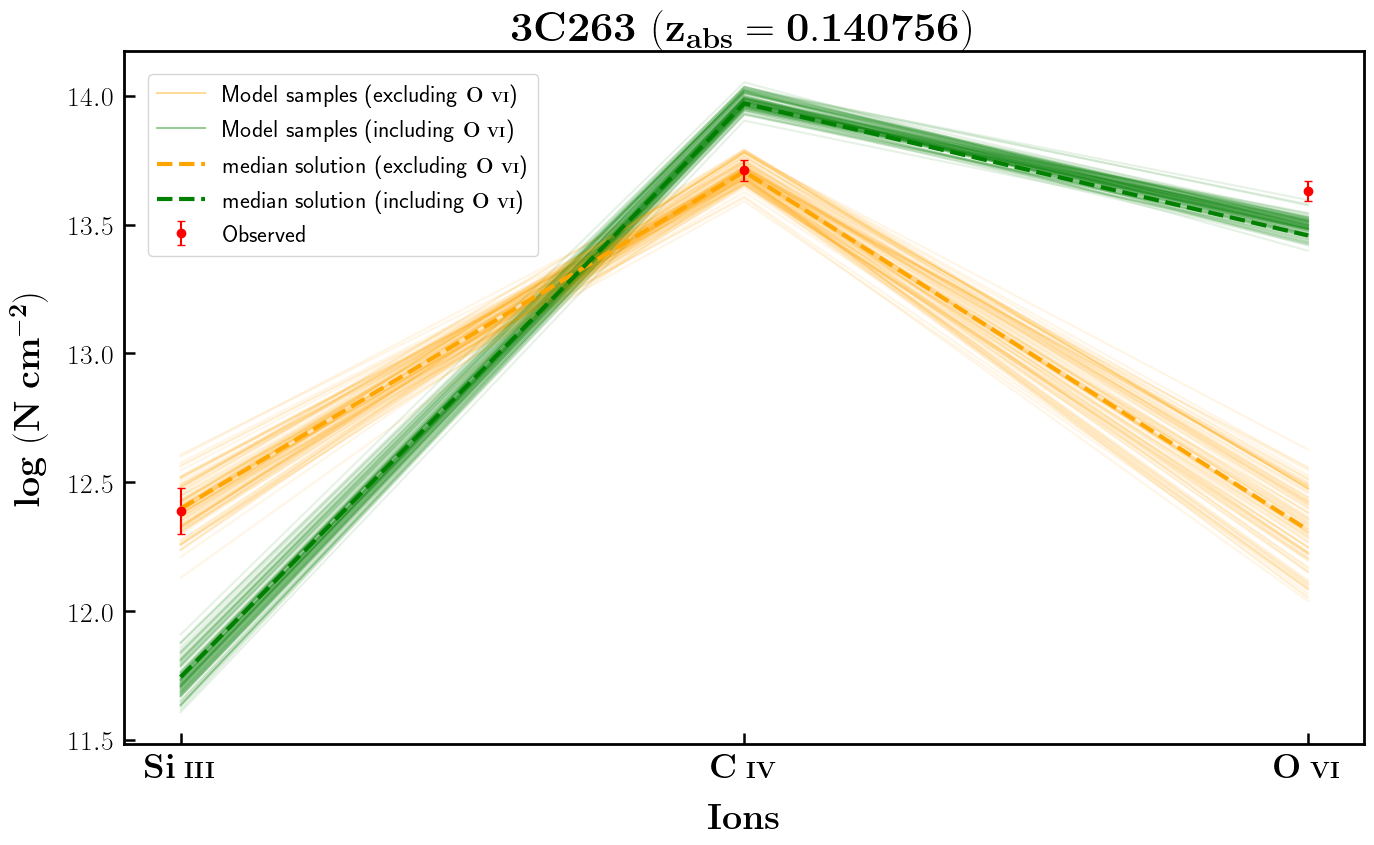
\includegraphics[width=0.9\linewidth]{Ionisation-Modelling-Plots/3c263-z=0.140756-compI_logZ=1.png}
      \caption{$\log \text{N}(\ion{H}{i}) \ [\text{cm}^{-2}]=$ 13.49}
  \end{figure}
  
    
  
  \newpage
  \thispagestyle{empty}
  
  \begin{landscape}
  
      \begin{figure}
      \centering
      \vspace{-10mm}
      \hspace*{-20mm}
      \captionsetup{oneside,margin={0cm,20mm}}
      \includegraphics[width=1.1\linewidth]{System-Plots/PKS0637-752_z=0.161064_sys_plot.png}
      \caption{System plot for the absorber along the LOS of PKS 0637-752 at $z_{abs} = 0.161064$. }
      \end{figure}
      
  \end{landscape}
  
  
  \begin{center}
   
  \begin{tabular}{cccc}
          \hline \hline \tabularnewline
          \head{Ion} & \head{v (km s\textsuperscript{$\mathbf{-1}$})} & \head{b (km s\textsuperscript{$\mathbf{-1}$})} & \head{log [N cm\textsuperscript{$\mathbf{-2}$}]} 
          \tabularnewline \tabularnewline \hline \tabularnewline 
  
          \ion{N}{v}   &    -42 $\pm$ 6    &    40 $\pm$ 9    &     13.37 $\pm$ 0.07 \\
          \ion{Si}{iii}   &    11 $\pm$ 4    &    30 $\pm$ 7    &     12.37 $\pm$ 0.06 \\
          \ion{O}{vi}   &    0 $\pm$ 3    &    48 $\pm$ 5    &     14.02 $\pm$ 0.03 \\
          \ion{H}{i}   &    -13 $\pm$ 2    &    162 $\pm$ 21    &     13.6 $\pm$ 0.06 \\
          \ion{H}{i}   &    -1 $\pm$ 1    &    45 $\pm$ 1    &     15.01 $\pm$ 0.02 \\
  \tabularnewline \hline \hline \tabularnewline
  
  \end{tabular}
  
  \end{center}
  
  $\log \text{N}(\ion{H}{i}) \ [\text{cm}^{-2}]=$ 13.60 \\
  
  Excluding \ion{O}{vi} : $\log n_H \ (\text{cm}^{-3})$ = -4.29 $\pm$ 0.02 \hspace{10mm} $\log \ Z/Z_\odot$ = 1.64 $\pm$ 0.05
  
  Including \ion{O}{vi} : $\log n_H \ (\text{cm}^{-3})$ = -4.42 $\pm$ 0.01 \hspace{10mm} $\log \ Z/Z_\odot$ = 1.69 $\pm$ 0.04 \\
  
  
  \begin{figure}[!h]
    \centering
    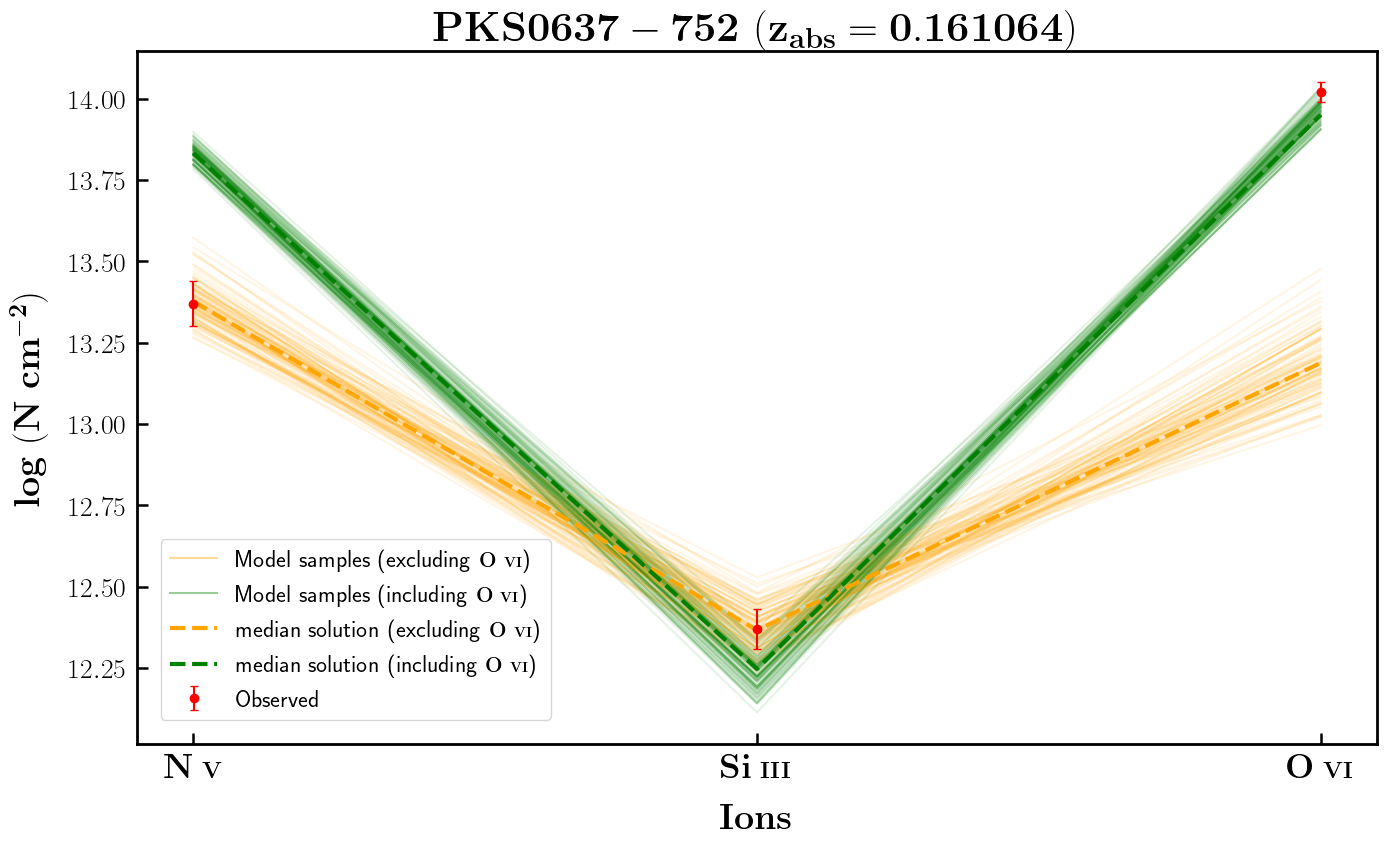
\includegraphics[width=0.9\linewidth]{Ionisation-Modelling-Plots/pks0637-z=0.161064-compI_logZ=1.png}
    \caption{$\log \text{N}(\ion{H}{i}) \ [\text{cm}^{-2}]=$ 13.60}
  \end{figure}
  
  
  
  \newpage
  \thispagestyle{empty}
  
  \begin{landscape}
  
      \begin{figure}
      \centering
      \vspace{-10mm}
      \hspace*{-20mm}
      \captionsetup{oneside,margin={0cm,20mm}}
      \includegraphics[width=1.1\linewidth]{System-Plots/PKS0637-752_z=0.417539_sys_plot.png}
      \caption{System plot for the absorber along the LOS of PKS 0637-752 at $z_{abs} = 0.417539$. }
      \end{figure}
      
  \end{landscape}
  
  
  \begin{center}
      
      \begin{tabular}{cccc}
          \hline \hline \tabularnewline
          \head{Ion} & \head{v (km s\textsuperscript{$\mathbf{-1}$})} & \head{b (km s\textsuperscript{$\mathbf{-1}$})} & \head{log [N cm\textsuperscript{$\mathbf{-2}$}]} 
          \tabularnewline \tabularnewline \hline \tabularnewline 
      
          \ion{Si}{iii}   &    -5 $\pm$ 4    &    35 $\pm$ 7    &     12.74 $\pm$ 0.06 \\
          \ion{C}{iii}   &    -4 $\pm$ 1    &    24 $\pm$ 2    &     14.44 $\pm$ 0.15 \\
          \ion{O}{vi}   &    0 $\pm$ 1    &    42 $\pm$ 6    &     14.19 $\pm$ 0.05 \\
          \ion{H}{i}   &    -17 $\pm$ 1    &    30 $\pm$ 1    &     15.41 $\pm$ 0.03 \\
          \ion{H}{i}   &    20 $\pm$ 1    &    46 $\pm$ 4    &     14.61 $\pm$ 0.07 \\
          
          \tabularnewline \hline \hline \tabularnewline
      
      \end{tabular}
      
  \end{center}
      
  $\log \text{N}(\ion{H}{i}) \ [\text{cm}^{-2}]=$ 15.41 \\
  
  Excluding \ion{O}{vi} : $\log n_H \ (\text{cm}^{-3})$ = -3.54 $\pm$ 0.11 \hspace{10mm} $\log \ Z/Z_\odot$ = -0.49 $\pm$ 0.11
  
  Including \ion{O}{vi} : $\log n_H \ (\text{cm}^{-3})$ = -3.74 $\pm$ 0.02 \hspace{10mm} $\log \ Z/Z_\odot$ = -0.23 $\pm$ 0.04 \\
  
  
  \begin{figure}[!h]
    \centering
    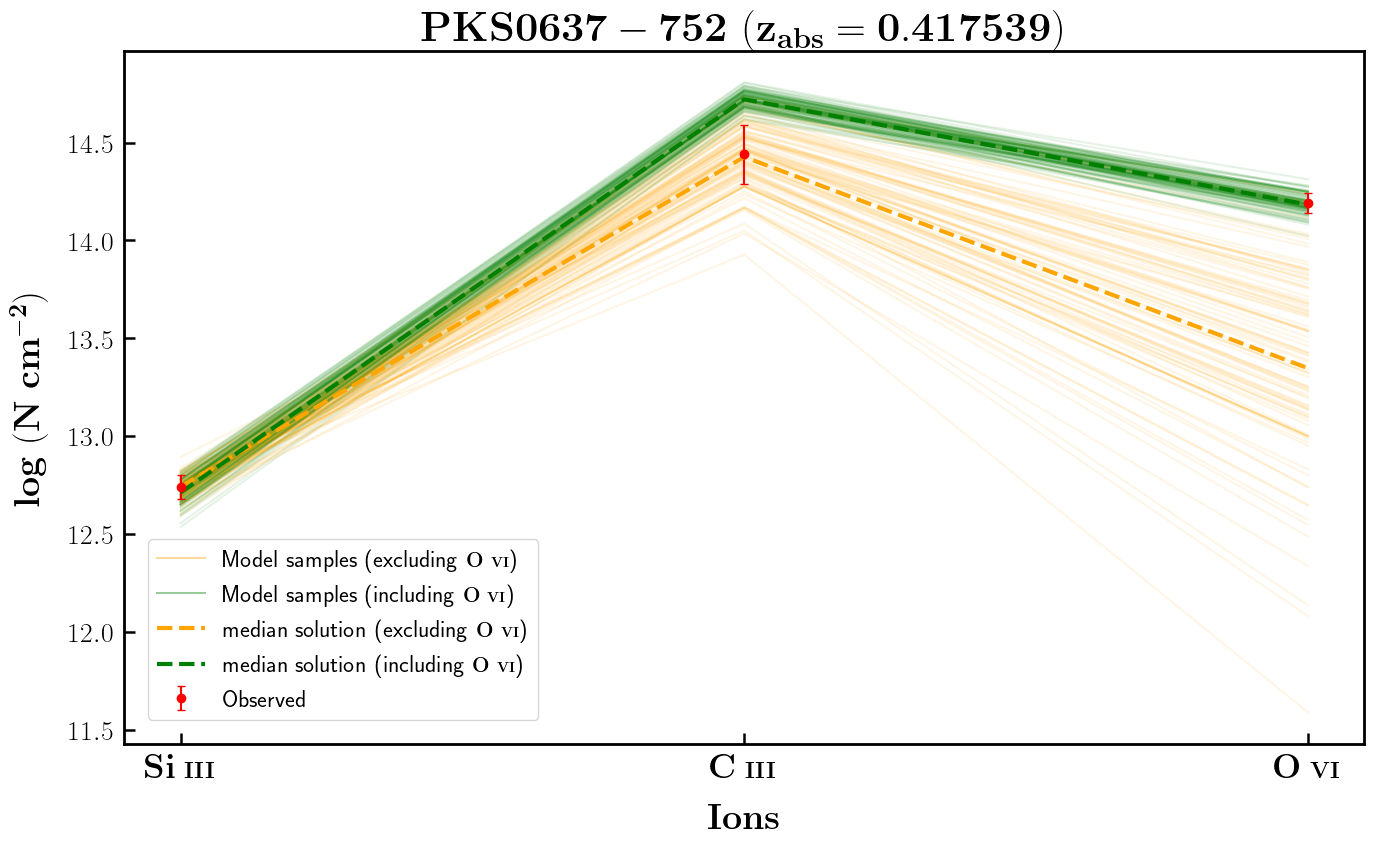
\includegraphics[width=0.9\linewidth]{Ionisation-Modelling-Plots/pks0637-z=0.417539-compI.png}
    \caption{$\log \text{N}(\ion{H}{i}) \ [\text{cm}^{-2}]=$ 15.41}
  \end{figure}
  
  
  \newpage
  \thispagestyle{empty}
  
  \begin{landscape}
  
      \begin{figure}
      \centering
      \vspace{-10mm}
      \hspace*{-20mm}
      \captionsetup{oneside,margin={0cm,20mm}}
      \includegraphics[width=1.1\linewidth]{System-Plots/PG1424+240_z=0.147104_sys_plot.png}
      \caption{System plot for the absorber along the LOS of PG 1424+240 at $z_{abs} = 0.147104$. }
      \end{figure}
      
  \end{landscape}
  
  
  \begin{center}
      
      \begin{tabular}{cccc}
              \hline \hline \tabularnewline
              \head{Ion} & \head{v (km s\textsuperscript{$\mathbf{-1}$})} & \head{b (km s\textsuperscript{$\mathbf{-1}$})} & \head{log [N cm\textsuperscript{$\mathbf{-2}$}]} 
              \tabularnewline \tabularnewline \hline \tabularnewline 
      
              \ion{C}{iv}   &    -81 $\pm$ 2    &    11 $\pm$ 4    &     13.58 $\pm$ 0.09 \\
              \ion{C}{iv}   &    -18 $\pm$ 2    &    20 $\pm$ 3    &     14.06 $\pm$ 0.05 \\ \tabularnewline
              \ion{Si}{iii}   &    -78 $\pm$ 2    &    15 $\pm$ 3    &     12.58 $\pm$ 0.05 \\
              \ion{Si}{iii}   &    -9 $\pm$ 1    &    16 $\pm$ 2    &     12.87 $\pm$ 0.03 \\ \tabularnewline
              \ion{Si}{iv}   &    -82 $\pm$ 4    &    13 $\pm$ 7    &     12.69 $\pm$ 0.1 \\
              \ion{Si}{iv}   &    -11 $\pm$ 2    &    11 $\pm$ 5    &     12.88 $\pm$ 0.07 \\ \tabularnewline
              \ion{O}{vi}   &    -56 $\pm$ 9    &    39 $\pm$ 13    &     13.77 $\pm$ 0.11 \\
              \ion{O}{vi}   &    4 $\pm$ 4    &    16 $\pm$ 6    &     13.73 $\pm$ 0.11 \\ \tabularnewline
              \ion{H}{i}   &    -454 $\pm$ 3    &    27 $\pm$ 5    &     13.16 $\pm$ 0.05 \\
              \ion{H}{i}   &    -87 $\pm$ 3    &    23 $\pm$ 2    &     14.88 $\pm$ 0.05 \\
              \ion{H}{i}   &    0 $\pm$ 3    &    29 $\pm$ 2    &     15.44 $\pm$ 0.14 \\
              \ion{H}{i}   &    216 $\pm$ 2    &    40 $\pm$ 3    &     13.49 $\pm$ 0.02 \\
              \tabularnewline \hline \hline \tabularnewline
      
      \end{tabular}
  
  \end{center}
  
  $\log \text{N}(\ion{H}{i}) \ [\text{cm}^{-2}]=$ 15.44 \\
  
  Excluding \ion{O}{vi} : $\log n_H \ (\text{cm}^{-3})$ = -3.81 $\pm$ 0.03 \hspace{10mm} $\log \ Z/Z_\odot$ = -0.46 $\pm$ 0.03
  
  Including \ion{O}{vi} : $\log n_H \ (\text{cm}^{-3})$ = -3.88 $\pm$ 0.02 \hspace{10mm} $\log \ Z/Z_\odot$ = -0.42 $\pm$ 0.02 \\
  
  $\log \text{N}(\ion{H}{i}) \ [\text{cm}^{-2}]=$ 14.88 \\
  
  Excluding \ion{O}{vi} : $\log n_H \ (\text{cm}^{-3})$ = -3.74 $\pm$ 0.05 \hspace{10mm} $\log \ Z/Z_\odot$ = -0.22 $\pm$ 0.04
  
  Including \ion{O}{vi} : $\log n_H \ (\text{cm}^{-3})$ = -3.96 $\pm$ 0.03 \hspace{10mm} $\log \ Z/Z_\odot$ = -0.07 $\pm$ 0.04
  
  \newpage
  
  \begin{figure}[!h]
    \centering
      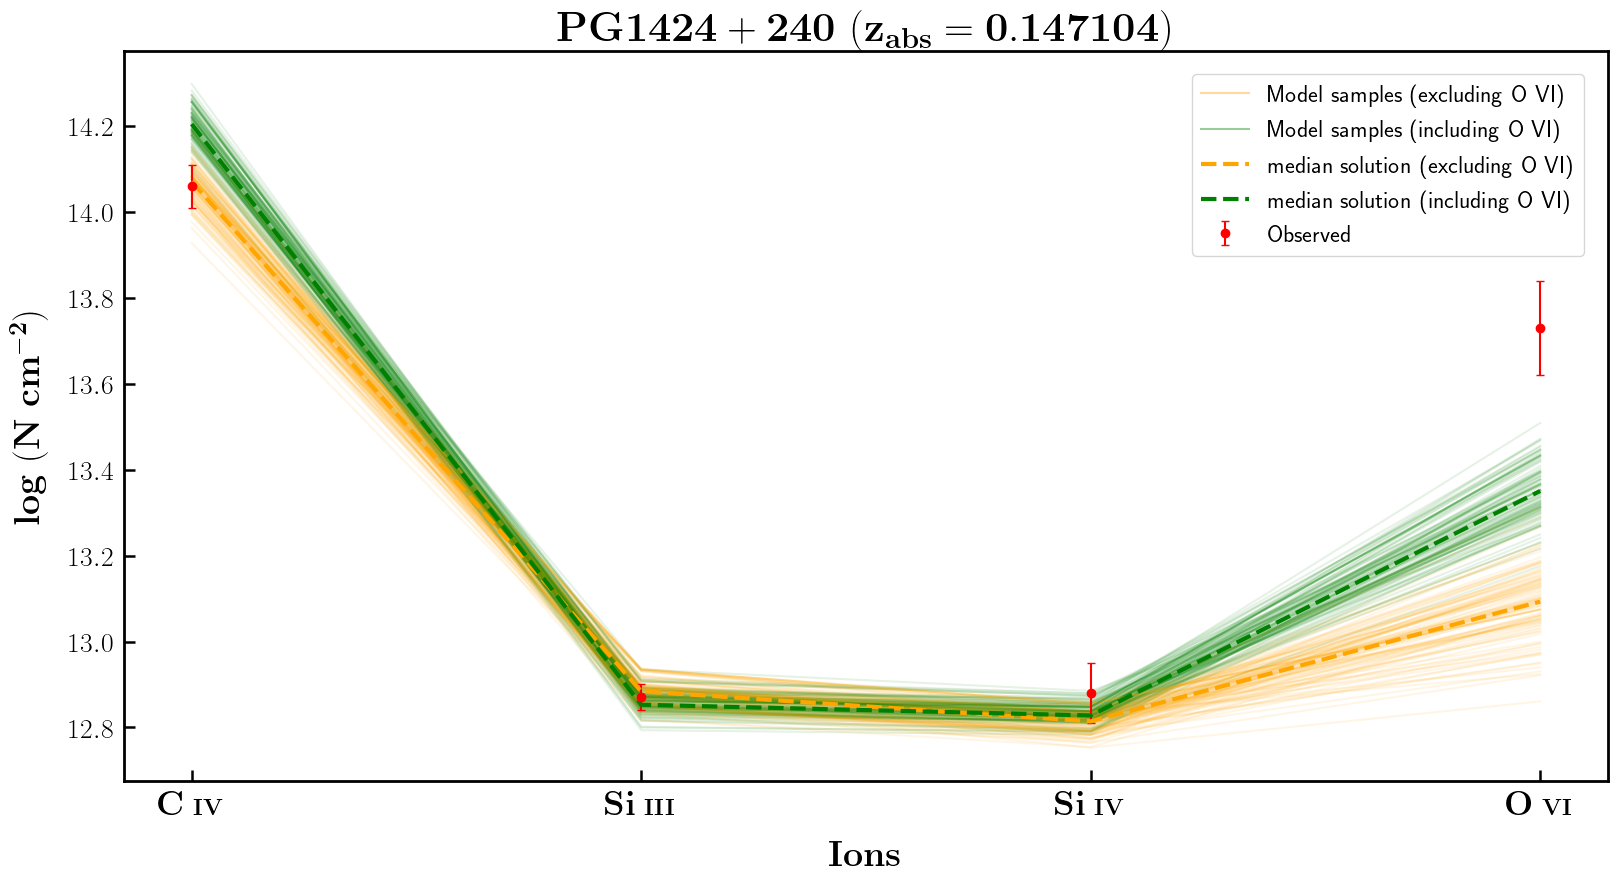
\includegraphics[width=0.9\linewidth]{Ionisation-Modelling-Plots/pg1424-z=0.147104-compIII.png}
      \caption{$\log \text{N}(\ion{H}{i}) \ [\text{cm}^{-2}]=$ 15.44}
  \end{figure}
  
  \begin{figure}[!b]
    \centering
      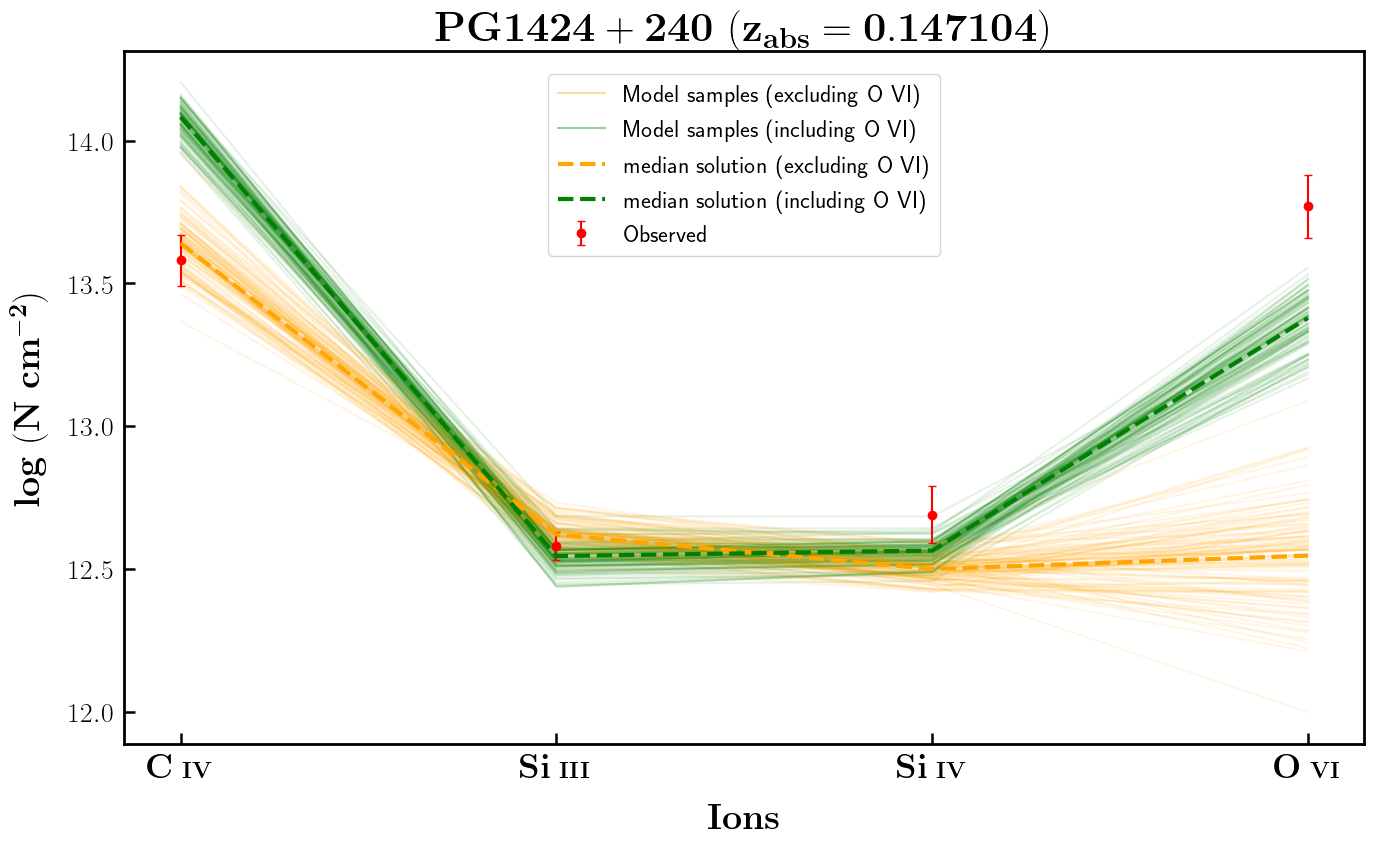
\includegraphics[width=0.9\linewidth]{Ionisation-Modelling-Plots/pg1424-z=0.147104-compII.png}
      \caption{$\log \text{N}(\ion{H}{i}) \ [\text{cm}^{-2}]=$ 14.88}
  \end{figure}
  
  
  \newpage
  \thispagestyle{empty}
  
  \begin{landscape}
  
      \begin{figure}
      \centering
      \vspace{-10mm}
      \hspace*{-20mm}
      \captionsetup{oneside,margin={0cm,20mm}}
      \includegraphics[width=1.1\linewidth]{System-Plots/PG0003+158_z=0.386089_sys_plot.png}
      \caption{System plot for the absorber along the LOS of PG 0003+158 at $z_{abs} = 0.386089$. }
      \end{figure}
      
  \end{landscape}
  
  \newgeometry{bottom=0.1cm}
  
  \begin{center}
      
      \begin{tabular}{cccc}
          \hline \hline \tabularnewline
          \head{Ion} & \head{v (km s\textsuperscript{$\mathbf{-1}$})} & \head{b (km s\textsuperscript{$\mathbf{-1}$})} & \head{log [N cm\textsuperscript{$\mathbf{-2}$}]} 
          \tabularnewline \tabularnewline \hline \tabularnewline 
      
          \ion{O}{iii}   &    -18 $\pm$ 2    &    9 $\pm$ 5    &     13.93 $\pm$ 0.08 \\
          \ion{C}{iii}   &    -11 $\pm$ 1    &    13 $\pm$ 2    &     13.35 $\pm$ 0.05 \\
          \ion{N}{v}   &    -7 $\pm$ 1    &    33 $\pm$ 11    &     13.49 $\pm$ 0.11 \\
          \ion{O}{vi}   &    0 $\pm$ 2    &    25 $\pm$ 3    &     13.87 $\pm$ 0.04 \\
          \ion{O}{vi}   &    54 $\pm$ 3    &    25 $\pm$ 4    &     13.71 $\pm$ 0.06 \\
          \ion{H}{i}   &    -10 $\pm$ 1    &    29 $\pm$ 0    &     14.81 $\pm$ 0.03 \\
          \ion{H}{i}   &    40 $\pm$ 9    &    40 $\pm$ 4    &     14.1 $\pm$ 0.05 \\
  
          \tabularnewline \hline \hline \tabularnewline
      
      \end{tabular}
      
  \end{center}
      
  $\log \text{N}(\ion{H}{i}) \ [\text{cm}^{-2}]=$ 14.81 \\
  
  Excluding \ion{O}{vi} : $\log n_H \ (\text{cm}^{-3})$ = -4.12 $\pm$ 0.06 \hspace{10mm} $\log \ Z/Z_\odot$ = -0.65 $\pm$ 0.04
  
  Including \ion{O}{vi} : $\log n_H \ (\text{cm}^{-3})$ = -4.07 $\pm$ 0.02 \hspace{10mm} $\log \ Z/Z_\odot$ = -0.68 $\pm$ 0.03 \\
  
  \begin{figure}[!h]
    \centering
    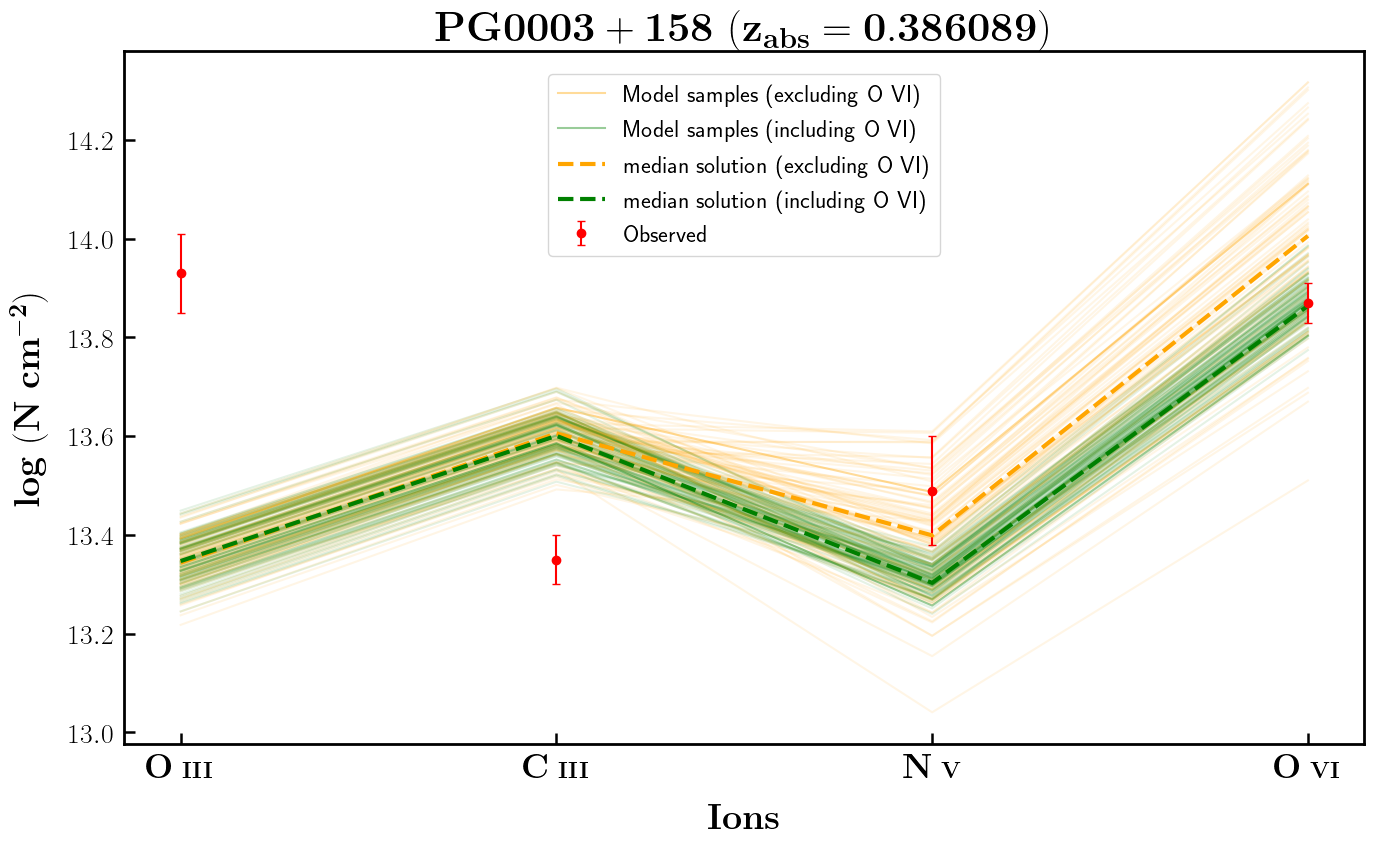
\includegraphics[width=0.9\linewidth]{Ionisation-Modelling-Plots/pg0003-z=0.386089-compI.png}
      \caption{$\log \text{N}(\ion{H}{i}) \ [\text{cm}^{-2}]=$ 14.81}
  \end{figure}
  
  \restoregeometry
  
  \newpage
  \thispagestyle{empty}
  
  \begin{landscape}
  
      \begin{figure}
      \centering
      \vspace{-10mm}
      \hspace*{-20mm}
      \captionsetup{oneside,margin={0cm,20mm}}
      \includegraphics[width=1.1\linewidth]{System-Plots/PG0003+158_z=0.421923_sys_plot.png}
      \caption{System plot for the absorber along the LOS of PG 0003+158 at $z_{abs} = 0.421923$. }
      \end{figure}
      
  \end{landscape}
  
  \newgeometry{bottom=0.1cm}
  
  \begin{center}
      
      \begin{tabular}{cccc}
          \hline \hline \tabularnewline
          \head{Ion} & \head{v (km s\textsuperscript{$\mathbf{-1}$})} & \head{b (km s\textsuperscript{$\mathbf{-1}$})} & \head{log [N cm\textsuperscript{$\mathbf{-2}$}]} 
          \tabularnewline \tabularnewline \hline \tabularnewline 
      
          \ion{C}{iii}   &    -9 $\pm$ 1    &    13 $\pm$ 1    &     13.35 $\pm$ 0.04 \\
          \ion{O}{iii}   &    -1 $\pm$ 2    &    7 $\pm$ 5    &     13.83 $\pm$ 0.13 \\
          \ion{O}{vi}   &    0 $\pm$ 1    &    27 $\pm$ 1    &     14.27 $\pm$ 0.02 \\
          \ion{H}{i}   &    -272 $\pm$ 6    &    66 $\pm$ 10    &     13.37 $\pm$ 0.05 \\
          \ion{H}{i}   &    -16 $\pm$ 1    &    64 $\pm$ 3    &     14.17 $\pm$ 0.04 \\
          \ion{H}{i}   &    -2 $\pm$ 1    &    26 $\pm$ 1    &     14.71 $\pm$ 0.02 \\
      
          \tabularnewline \hline \hline \tabularnewline
      
      \end{tabular}
      
  \end{center}
      
  $\log \text{N}(\ion{H}{i}) \ [\text{cm}^{-2}]=$ 14.17 \\
  
  Excluding \ion{O}{vi} : $\log n_H \ (\text{cm}^{-3})$ = -2.66 $\pm$ 0.22 \hspace{10mm} $\log \ Z/Z_\odot$ = 0.42 $\pm$ 0.23
  
  Including \ion{O}{vi} : $\log n_H \ (\text{cm}^{-3})$ = -4.24 $\pm$ 0.02 \hspace{10mm} $\log \ Z/Z_\odot$ = -0.09 $\pm$ 0.03 \\
  
  \begin{figure}[!h]
    \centering
    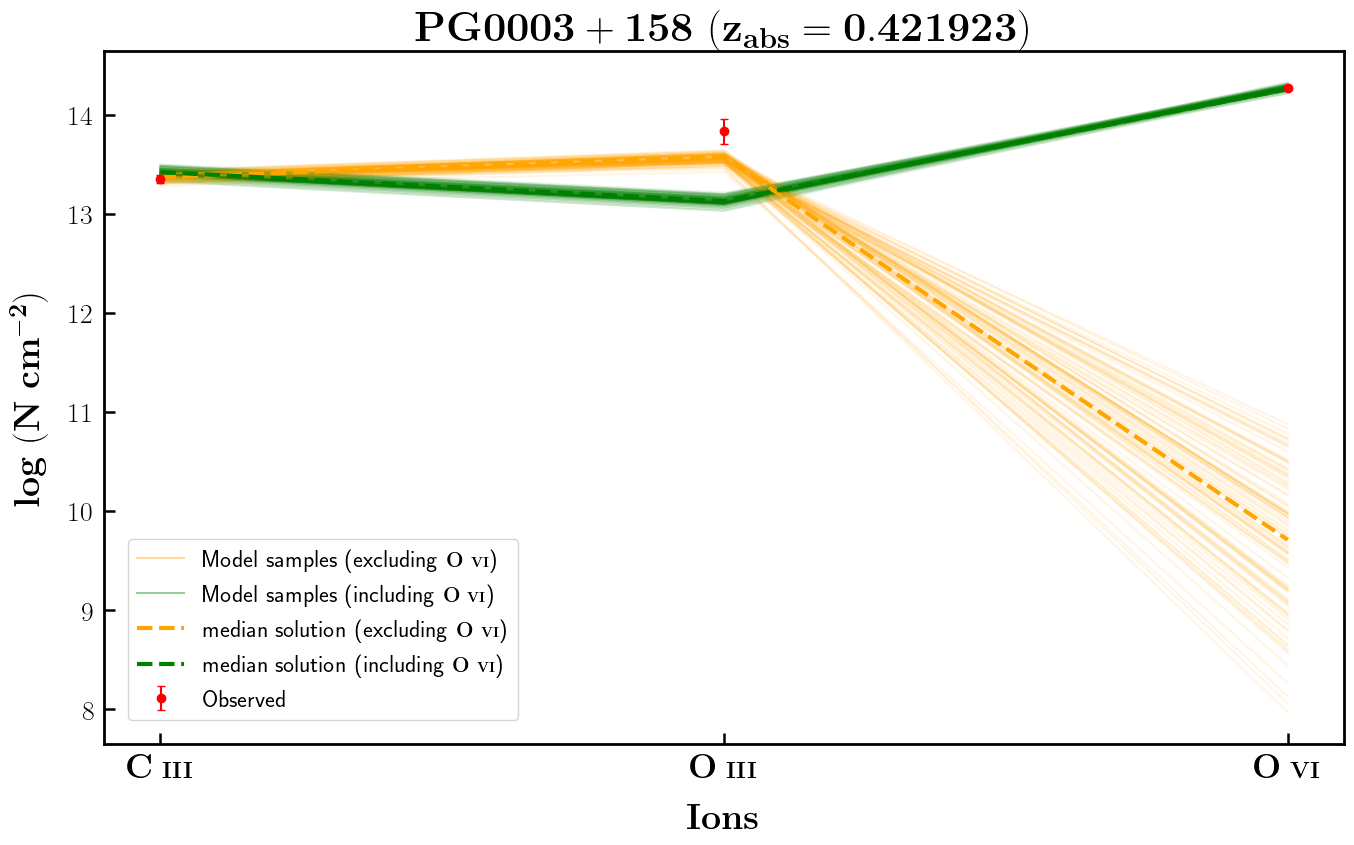
\includegraphics[width=0.9\linewidth]{Ionisation-Modelling-Plots/pg0003-z=0.421923-compII.png}
      \caption{$\log \text{N}(\ion{H}{i}) \ [\text{cm}^{-2}]=$ 14.17}
  \end{figure}

  \restoregeometry
  
  
  \newpage
  \thispagestyle{empty}
  
  \begin{landscape}
  
      \begin{figure}
      \centering
      \vspace{-10mm}
      \hspace*{-20mm}
      \captionsetup{oneside,margin={0cm,20mm}}
      \includegraphics[width=1.1\linewidth]{System-Plots/PG1216+069_z=0.282286_sys_plot.png}
      \caption{System plot for the absorber along the LOS of PG 1216+069 at $z_{abs} = 0.282286$. }
      \end{figure}
      
  \end{landscape}
  
  
  \begin{center}
   
  \begin{tabular}{cccc}
          \hline \hline \tabularnewline
          \head{Ion} & \head{v (km s\textsuperscript{$\mathbf{-1}$})} & \head{b (km s\textsuperscript{$\mathbf{-1}$})} & \head{log [N cm\textsuperscript{$\mathbf{-2}$}]} 
          \tabularnewline \tabularnewline \hline \tabularnewline 
  
          \ion{Si}{iii}   &    0 $\pm$ 1    &    14 $\pm$ 3    &     12.92 $\pm$ 0.05 \\
          \ion{C}{iii}   &    -51 $\pm$ 3    &    32 $\pm$ 5    &     13.33 $\pm$ 0.05 \\
          \ion{C}{iii}   &    5 $\pm$ 1    &    16 $\pm$ 2    &     13.76 $\pm$ 0.07 \\
          \ion{O}{vi}   &    -64 $\pm$ 6    &    58 $\pm$ 9    &     13.93 $\pm$ 0.05 \\
          \ion{O}{vi}   &    19 $\pm$ 2    &    12 $\pm$ 5    &     13.54 $\pm$ 0.09 \\
          \ion{H}{i}   &    -31 $\pm$ 1    &    52 $\pm$ 3    &     15.1 $\pm$ 0.05 \\
          \ion{H}{i}   &    7 $\pm$ 1    &    22 $\pm$ 1    &     16.4 $\pm$ 0.03 \\
          \ion{H}{i}   &    169 $\pm$ 22    &    53 $\pm$ 10    &     13.15 $\pm$ 0.18 \\
  
          \tabularnewline \hline \hline \tabularnewline
  
  \end{tabular}
      
  \end{center}
      
  $\log \text{N}(\ion{H}{i}) \ [\text{cm}^{-2}]=$ 15.10 \\
  
  Excluding \ion{O}{vi} : $\log n_H \ (\text{cm}^{-3})$ = -2.13 $\pm$ 0.15 \hspace{10mm} $\log \ Z/Z_\odot$ = 0.65 $\pm$ 0.22
  
  Including \ion{O}{vi} : $\log n_H \ (\text{cm}^{-3})$ = -3.86 $\pm$ 0.02 \hspace{10mm} $\log \ Z/Z_\odot$ = -0.37 $\pm$ 0.03 \\
  
  $\log \text{N}(\ion{H}{i}) \ [\text{cm}^{-2}]=$ 16.40 \\
  
  Excluding \ion{O}{vi} : $\log n_H \ (\text{cm}^{-3})$ = -2.08 $\pm$ 0.43 \hspace{10mm} $\log \ Z/Z_\odot$ = -0.37 $\pm$ 0.59
  
  Including \ion{O}{vi} : $\log n_H \ (\text{cm}^{-3})$ = -3.68 $\pm$ 0.02 \hspace{10mm} $\log \ Z/Z_\odot$ = -1.55 $\pm$ 0.04 
  \newpage
  
  
  \begin{figure}[!h]
      \centering
      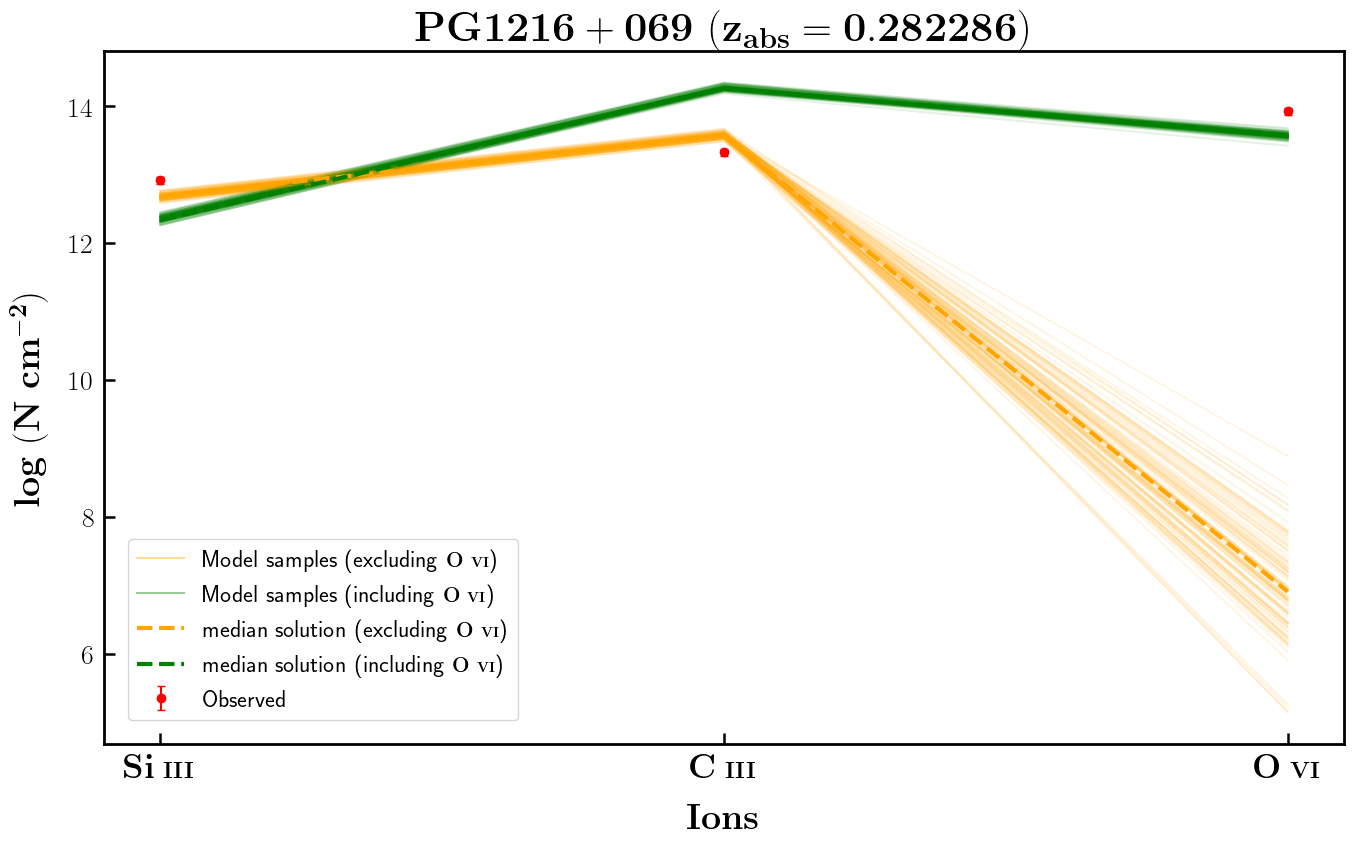
\includegraphics[width=0.9\linewidth]{Ionisation-Modelling-Plots/pg1216-z=0.282286-compI.png}
      \caption{$\log \text{N}(\ion{H}{i}) \ [\text{cm}^{-2}]=$ 15.10}
  \end{figure}
  
  \begin{figure}[!b]
      \centering
      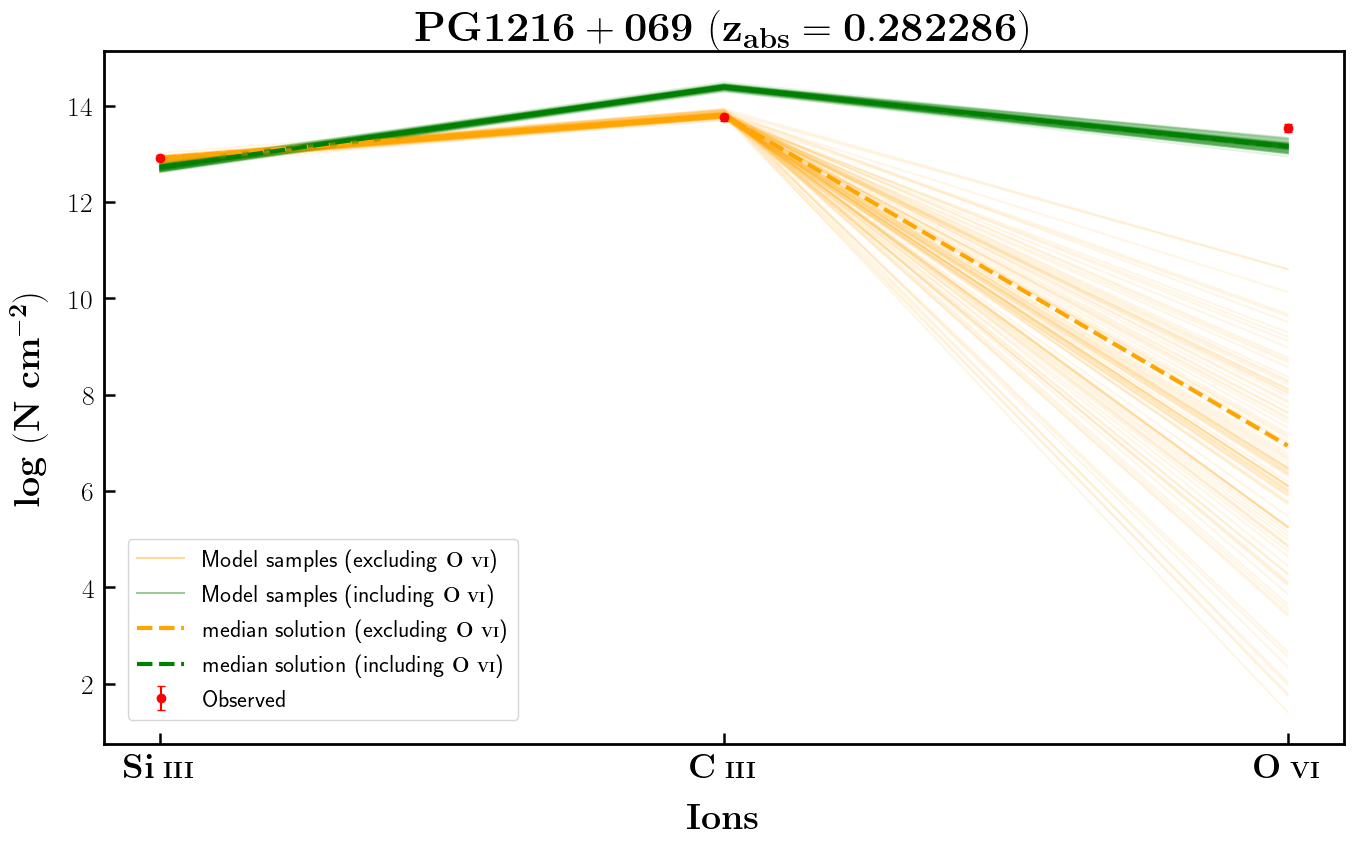
\includegraphics[width=0.9\linewidth]{Ionisation-Modelling-Plots/pg1216-z=0.282286-compII.png}
      \caption{$\log \text{N}(\ion{H}{i}) \ [\text{cm}^{-2}]=$ 16.40}
  \end{figure}
  
  
  \newpage
  \thispagestyle{empty}
  
  \begin{landscape}
  
  \begin{figure}
      \centering
      \vspace{-10mm}
      \hspace*{-20mm}
      \captionsetup{oneside,margin={0cm,20mm}}
      \includegraphics[width=1.1\linewidth]{System-Plots/SDSSJ135712.61+170444_z=0.097869_sys_plot.png}
      \caption{System plot for the absorber along the LOS of SDSS J135712.61+170444 at $z_{abs} = 0.097869$. }
  \end{figure}
  
  \end{landscape}
  
  \newgeometry{top=22mm,bottom=0.1cm}
  
  \begin{center} 
  
  \begin{tabular}{cccc} 
  
      \hline \hline \tabularnewline 
      \head{Ion} & \head{v (km s\textsuperscript{$\mathbf{-1}$})} & \head{b (km s\textsuperscript{$\mathbf{-1}$})} & \head{log [N cm\textsuperscript{$\mathbf{-2}$}]}
      \tabularnewline \tabularnewline \hline \tabularnewline 
   
      \ion{Si}{iii}   &    -62 $\pm$ 2    &    17 $\pm$ 3    &     12.94 $\pm$ 0.05 \\
      \ion{Si}{iii}   &    4 $\pm$ 1    &    13 $\pm$ 10    &     14.67 $\pm$ 2.87 \\
      \ion{C}{iv}   &    -74 $\pm$ 6    &    33 $\pm$ 1    &     13.82 $\pm$ 0.09 \\
      \ion{C}{iv}   &    -7 $\pm$ 8    &    32 $\pm$ 12    &     13.63 $\pm$ 0.12 \\
      \ion{Si}{iv}   &    -66 $\pm$ 4    &    18 $\pm$ 6    &     13.02 $\pm$ 0.08 \\
      \ion{Si}{iv}   &    0 $\pm$ 4    &    29 $\pm$ 5    &     13.3 $\pm$ 0.05 \\
      \ion{C}{ii}   &    -79 $\pm$ 8    &    19 $\pm$ 14    &     13.17 $\pm$ 0.16 \\
      \ion{C}{ii}   &    -1 $\pm$ 2    &    22 $\pm$ 3    &     13.92 $\pm$ 0.04 \\
      \ion{O}{vi}   &    -96 $\pm$ 10    &    43 $\pm$ 16    &     14.3 $\pm$ 0.11 \\
      \ion{H}{i}   &    -536 $\pm$ 3    &    29 $\pm$ 5    &     13.36 $\pm$ 0.05 \\
      \ion{H}{i}   &    -66 $\pm$ 0    &    29 $\pm$ 8    &     16.49 $\pm$ 0.12 \\
      \ion{H}{i}   &    0 $\pm$ 0    &    46 $\pm$ 4    &     15.01 $\pm$ 0.16 \\
      \ion{H}{i}   &    424 $\pm$ 3    &    34 $\pm$ 4    &     13.52 $\pm$ 0.04 \\
  
      \tabularnewline \hline \hline \tabularnewline 
  
  \end{tabular}
  
  \end{center}
  
  
  $\log \text{N}(\ion{H}{i}) \ [\text{cm}^{-2}]=$ 16.49 \\
  
  Excluding \ion{O}{vi} : $\log n_H \ (\text{cm}^{-3})$ = -3.76 $\pm$ 0.05 \hspace{10mm} $\log \ Z/Z_\odot$ = -1.49 $\pm$ 0.04
  
  Including \ion{O}{vi} : $\log n_H \ (\text{cm}^{-3})$ = -4.06 $\pm$ 0.02 \hspace{10mm} $\log \ Z/Z_\odot$ = -1.32 $\pm$ 0.04 \\
  
  \begin{figure}[!h]
      \centering
      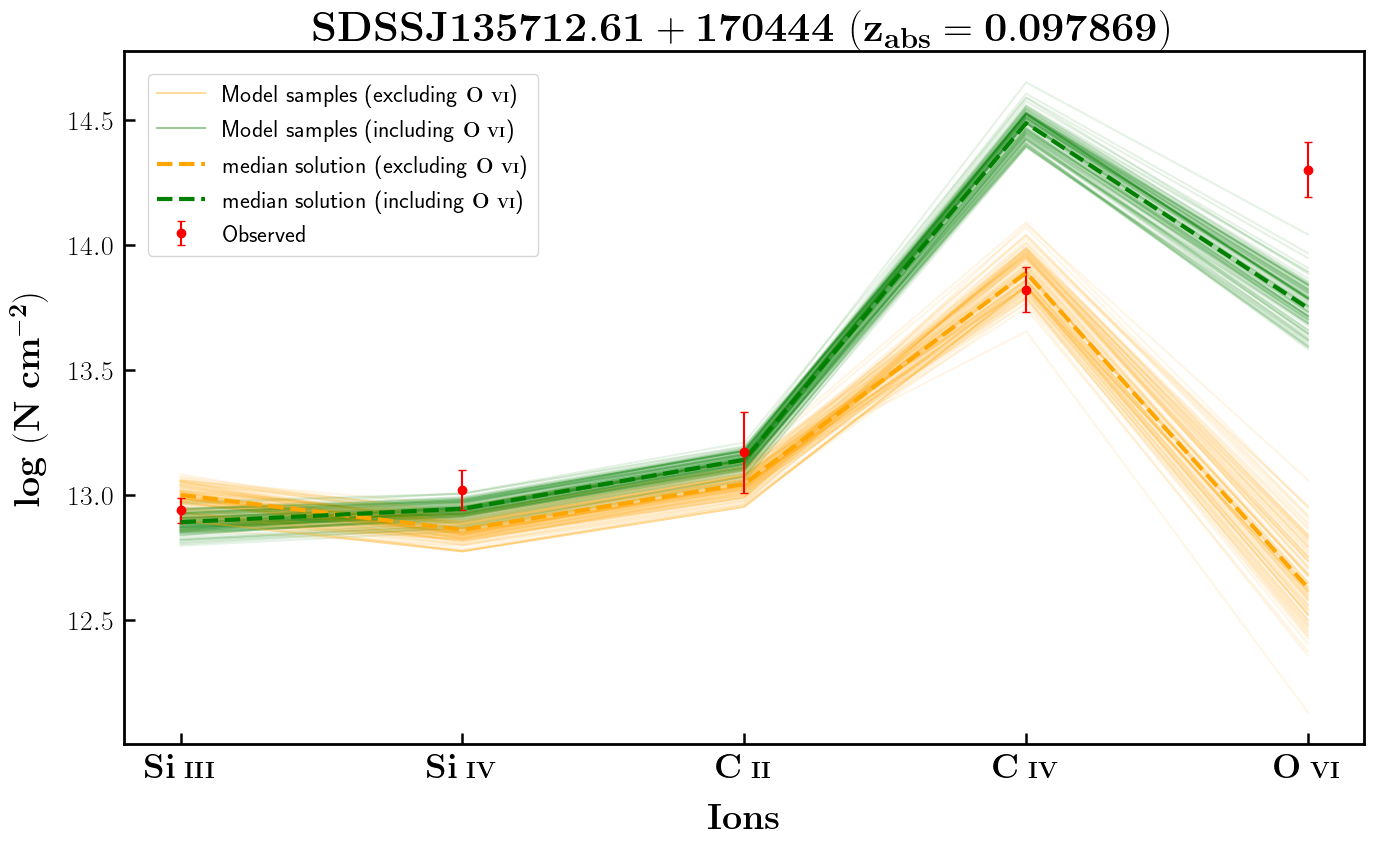
\includegraphics[width=0.9\linewidth]{Ionisation-Modelling-Plots/s135712-z=0.097869-compII.png}
      \caption{$\log \text{N}(\ion{H}{i}) \ [\text{cm}^{-2}]=$ 16.49}
  \end{figure}
  
  \restoregeometry
  
  \newpage
  \thispagestyle{empty}

  \begin{landscape}
  
  \begin{figure}
      \centering
      \vspace{-10mm}
      \hspace*{-20mm}
      \captionsetup{oneside,margin={0cm,20mm}}
      \includegraphics[width=1.1\linewidth]{System-Plots/1ES1553+113_z=0.187764_sys_plot.png}
      \caption{System plot for the absorber along the LOS of 1ES 1553+113 at $z_{abs} = 0.187764$. }
  \end{figure}
  
  \end{landscape}
  
  
  \begin{center} 
  
  \begin{tabular}{cccc} 
  
      \hline \hline \tabularnewline 
      \head{Ion} & \head{v (km s\textsuperscript{$\mathbf{-1}$})} & \head{b (km s\textsuperscript{$\mathbf{-1}$})} & \head{log [N cm\textsuperscript{$\mathbf{-2}$}]}
      \tabularnewline \tabularnewline \hline \tabularnewline 
   
      \ion{C}{iii}   &    -46 $\pm$ 1    &    5 $\pm$ 4    &     13.17 $\pm$ 0.46 \\
      \ion{C}{iii}   &    -6 $\pm$ 1    &    13 $\pm$ 2    &     13.21 $\pm$ 0.03 \\
      \ion{N}{v}   &    -47 $\pm$ 2    &    17 $\pm$ 0    &     13.43 $\pm$ 0.05 \\
      \ion{N}{v}   &    -5 $\pm$ 2    &    16 $\pm$ 4    &     13.33 $\pm$ 0.06 \\
      \ion{O}{vi}   &    -42 $\pm$ 1    &    3 $\pm$ 1    &     14.23 $\pm$ 0.33 \\
      \ion{O}{vi}   &    0 $\pm$ 1    &    15 $\pm$ 3    &     13.71 $\pm$ 0.03 \\
      \ion{O}{vi}   &    511 $\pm$ 3    &    28 $\pm$ 5    &     13.49 $\pm$ 0.05 \\
      \ion{H}{i}   &    -52 $\pm$ 3    &    8 $\pm$ 6    &     12.76 $\pm$ 0.15 \\
      \ion{H}{i}   &    -28 $\pm$ 1    &    51 $\pm$ 1    &     13.88 $\pm$ 0.01 \\
      \ion{H}{i}   &    425 $\pm$ 3    &    25 $\pm$ 5    &     13.02 $\pm$ 0.07 \\
      \ion{H}{i}   &    496 $\pm$ 2    &    37 $\pm$ 3    &     13.46 $\pm$ 0.03 \\
  
      \tabularnewline \hline \hline \tabularnewline 
  
  \end{tabular}
  
  \end{center}
  
  $\log \text{N}(\ion{H}{i}) \ [\text{cm}^{-2}]=$ 12.76 \\
  
  Excluding \ion{O}{vi} : $\log n_H \ (\text{cm}^{-3})$ = -4.62 $\pm$ 0.04 \hspace{10mm} $\log \ Z/Z_\odot$ = 1.37 $\pm$ 0.06
  
  Including \ion{O}{vi} : $\log n_H \ (\text{cm}^{-3})$ = -4.63 $\pm$ 0.03 \hspace{10mm} $\log \ Z/Z_\odot$ = 1.37 $\pm$ 0.06
  \\\\
  
  $\log \text{N}(\ion{H}{i}) \ [\text{cm}^{-2}]=$ 13.88 \\
  
  Excluding \ion{O}{vi} : $\log n_H \ (\text{cm}^{-3})$ = -4.6 $\pm$ 0.04 \hspace{10mm} $\log \ Z/Z_\odot$ = 0.03 $\pm$ 0.03
  
  Including \ion{O}{vi} : $\log n_H \ (\text{cm}^{-3})$ = -4.44 $\pm$ 0.02 \hspace{10mm} $\log \ Z/Z_\odot$ = -0.06 $\pm$ 0.02
  \\\\
  
  
  \newpage
  
  
  \begin{figure}[!h]
      \centering
      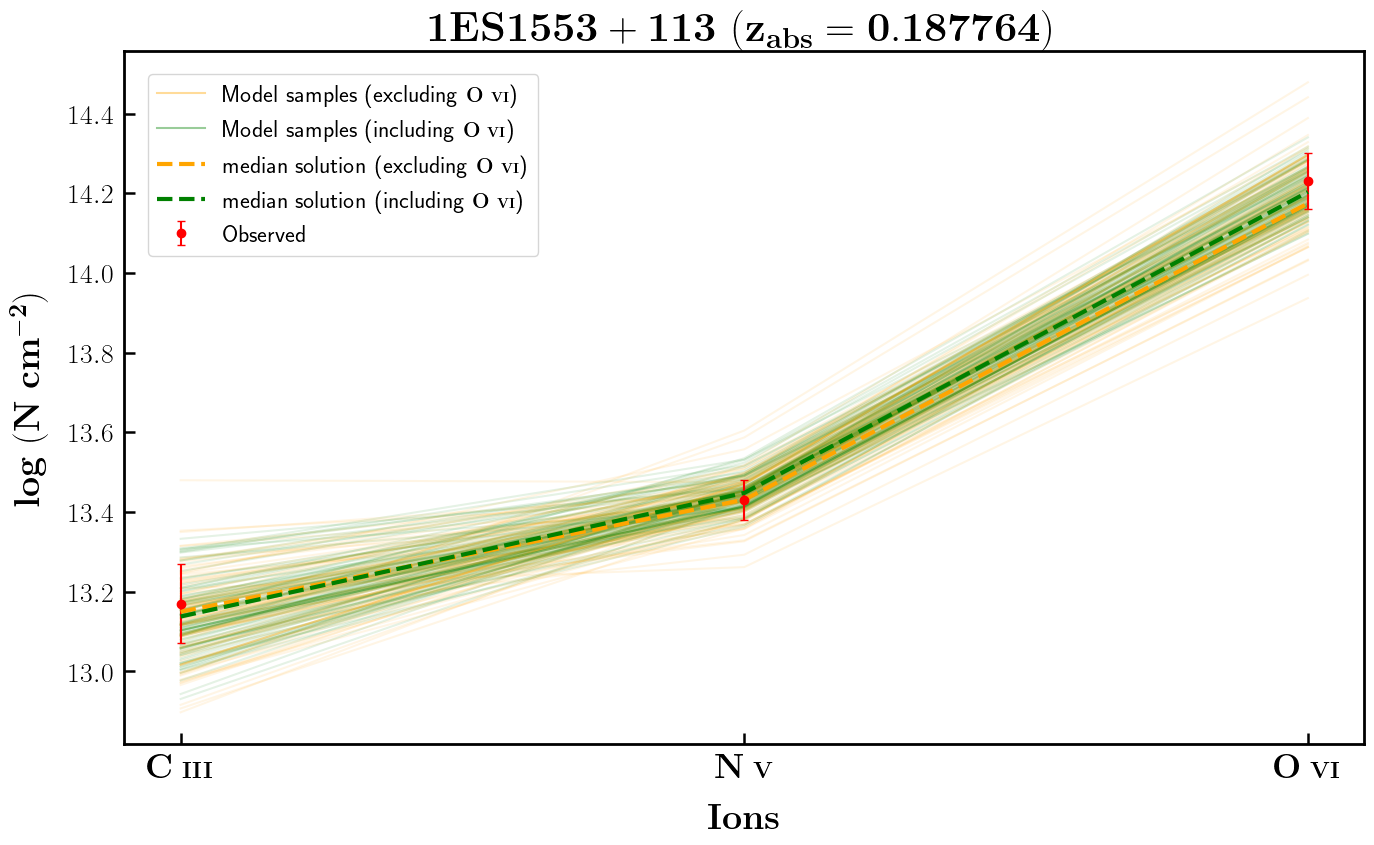
\includegraphics[width=0.9\linewidth]{Ionisation-Modelling-Plots/1es1553-z=0.187764-compI.png}
      \caption{$\log \text{N}(\ion{H}{i}) \ [\text{cm}^{-2}]=$ 12.76}
  \end{figure}
  
  \begin{figure}[!b]
      \centering
      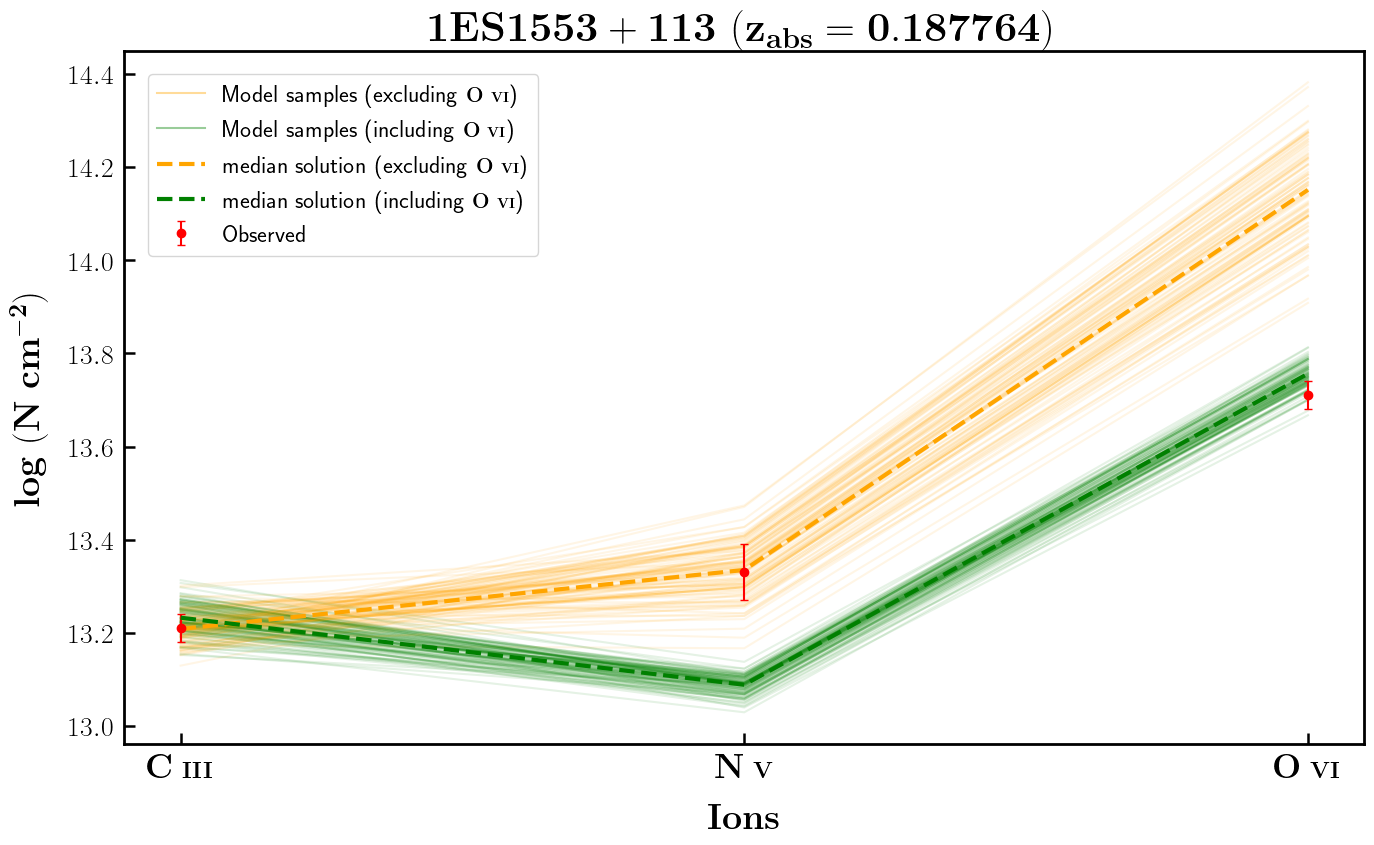
\includegraphics[width=0.9\linewidth]{Ionisation-Modelling-Plots/1es1553-z=0.187764-compII.png}
      \caption{$\log \text{N}(\ion{H}{i}) \ [\text{cm}^{-2}]=$ 13.88}
  \end{figure}
  
  
  
  \newpage
  \thispagestyle{empty}

  \begin{landscape}
  
  \begin{figure}
      \centering
      \vspace{-10mm}
      \hspace*{-20mm}
      \captionsetup{oneside,margin={0cm,20mm}}
      \includegraphics[width=1.1\linewidth]{System-Plots/SBS1108+560_z=0.463207_sys_plot.png}
      \caption{System plot for the absorber along the LOS of SBS 1108+560 at $z_{abs} = 0.463207$. }
  \end{figure}
  
  \end{landscape}
  
  
  \begin{center} 
  
  \begin{tabular}{cccc} 
  
      \hline \hline \tabularnewline 
      \head{Ion} & \head{v (km s\textsuperscript{$\mathbf{-1}$})} & \head{b (km s\textsuperscript{$\mathbf{-1}$})} & \head{log [N cm\textsuperscript{$\mathbf{-2}$}]}
      \tabularnewline \tabularnewline \hline \tabularnewline 
   
      \ion{O}{i}   &    25 $\pm$ 2    &    18 $\pm$ 4    &     14.13 $\pm$ 0.05 \\
      \ion{Si}{iii}   &    -23 $\pm$ 9    &    39 $\pm$ 12    &     13.26 $\pm$ 0.12 \\
      \ion{Si}{iii}   &    21 $\pm$ 2    &    13 $\pm$ 15    &     14.61 $\pm$ 0.24 \\
      \ion{C}{ii}   &    12 $\pm$ 9    &    31 $\pm$ 4    &     14.15 $\pm$ 0.05 \\
      \ion{C}{ii}   &    34 $\pm$ 2    &    12 $\pm$ 5    &     14.67 $\pm$ 0.1 \\
      \ion{C}{iii}   &    -48 $\pm$ 3    &    15 $\pm$ 1    &     13.66 $\pm$ 0.08 \\
      \ion{C}{iii}   &    -10 $\pm$ 3    &    26 $\pm$ 7    &     14.16 $\pm$ 0.07 \\
      \ion{C}{iii}   &    28 $\pm$ 3    &    24 $\pm$ 1    &     13.95 $\pm$ 0.05 \\
      \ion{N}{iii}   &    -22 $\pm$ 59    &    67 $\pm$ 61    &     13.77 $\pm$ 0.1 \\
      \ion{N}{iii}   &    32 $\pm$ 2    &    26 $\pm$ 4    &     14.49 $\pm$ 0.09 \\
      \ion{Si}{ii}   &    25 $\pm$ 1    &    15 $\pm$ 1    &     13.57 $\pm$ 0.08 \\
      \ion{O}{vi}   &    0 $\pm$ 6    &    45 $\pm$ 10    &     13.71 $\pm$ 0.07 \\
      \ion{H}{i}   &    -48 $\pm$ 0    &    22 $\pm$ 2    &     15.77 $\pm$ 0.02 \\
      \ion{H}{i}   &    -10 $\pm$ 2    &    16 $\pm$ 0    &     15.79 $\pm$ 0.11 \\
      \ion{H}{i}   &    28 $\pm$ 1    &    16 $\pm$ 1    &     18.1 $\pm$ 0.12 \\
      
      \tabularnewline \hline \hline \tabularnewline 
  
  \end{tabular}
  
  \end{center}
  
  
  $\log \text{N}(\ion{H}{i}) \ [\text{cm}^{-2}]=$ 18.10 \\
  
  Excluding \ion{O}{vi} : $\log n_H \ (\text{cm}^{-3})$ = -2.55 $\pm$ 0.03 \hspace{10mm} $\log \ Z/Z_\odot$ = -0.83 $\pm$ 0.04
  
  Including \ion{O}{vi} : $\log n_H \ (\text{cm}^{-3})$ = -3.49 $\pm$ 0.01 \hspace{10mm} $\log \ Z/Z_\odot$ = -0.92 $\pm$ 0.03
  \\
  
  $\log \text{N}(\ion{H}{i}) \ [\text{cm}^{-2}]=$ 15.79 \\
  
  Excluding \ion{O}{vi} : $\log n_H \ (\text{cm}^{-3})$ = -2.65 $\pm$ 0.22 \hspace{10mm} $\log \ Z/Z_\odot$ = 1.60 $\pm$ 0.22
  
  Including \ion{O}{vi} : $\log n_H \ (\text{cm}^{-3})$ = -3.56 $\pm$ 0.03 \hspace{10mm} $\log \ Z/Z_\odot$ = 1.16 $\pm$ 0.05
  
  
  \newpage
  
  \begin{figure}[!h]
    \centering
    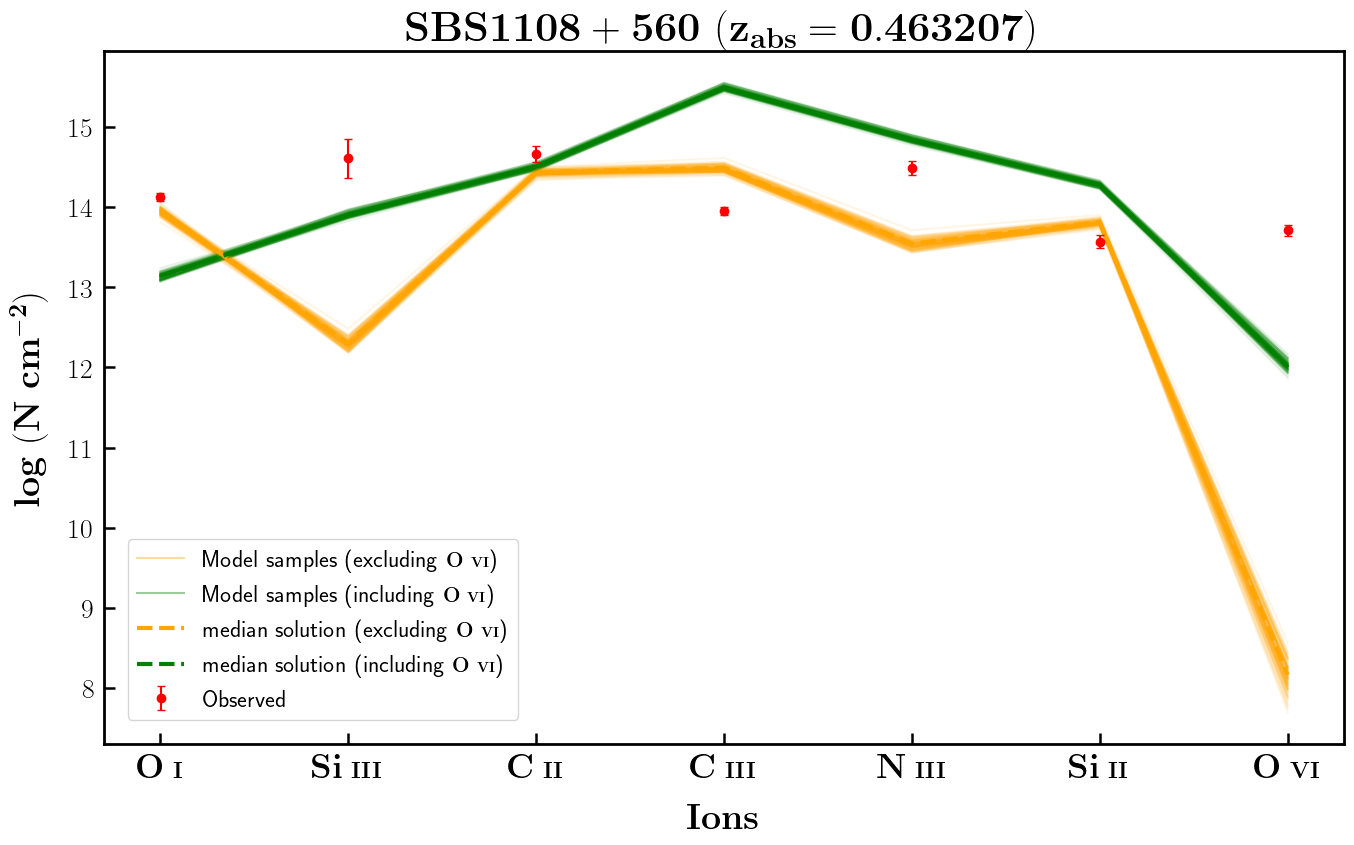
\includegraphics[width=0.9\linewidth]{Ionisation-Modelling-Plots/sbs1108-z=0.463207-compIII_logZ=1.png}
    \caption{$\log \text{N}(\ion{H}{i}) \ [\text{cm}^{-2}]=$ 18.10}
  \end{figure}
  
  
  \begin{figure}[!b]
      \centering
      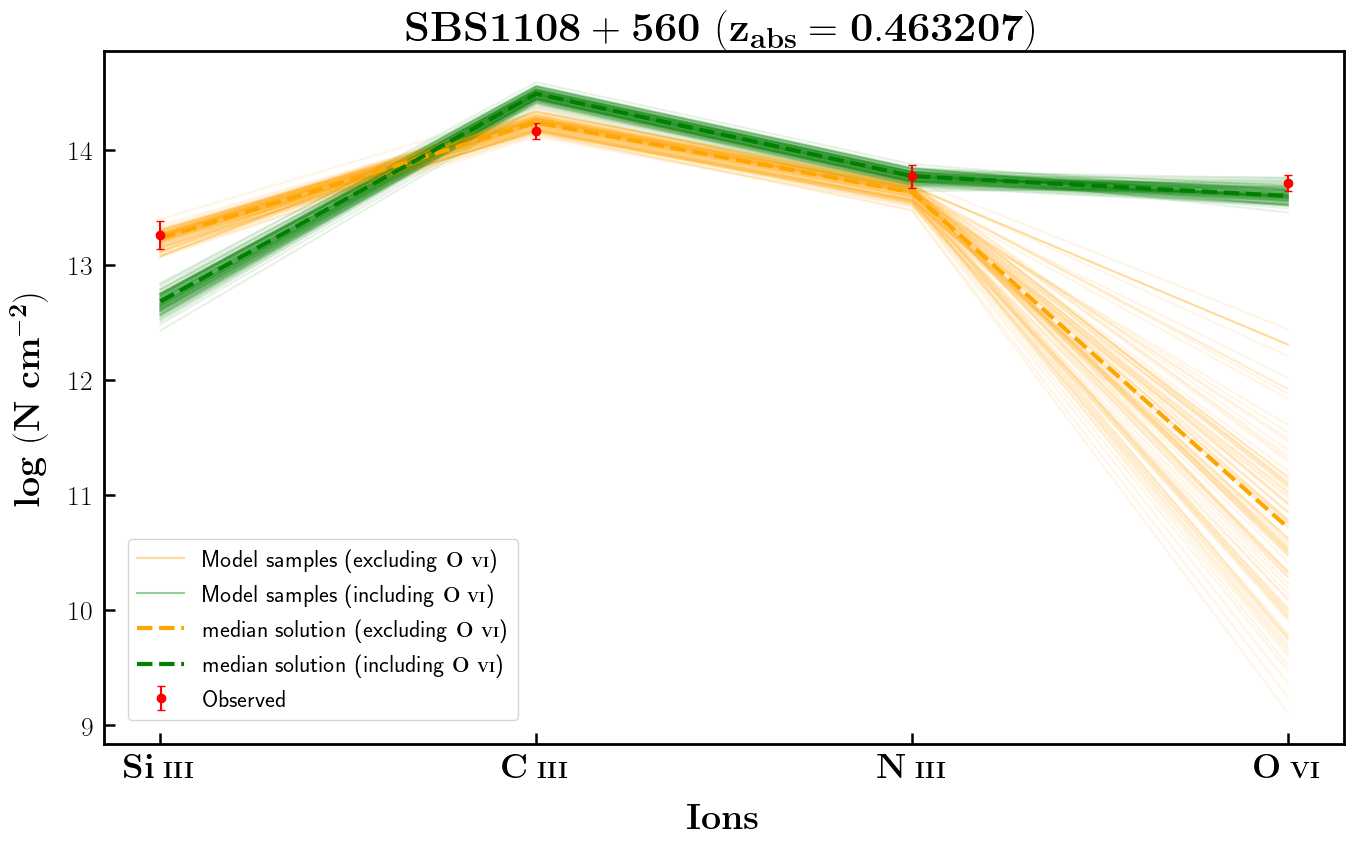
\includegraphics[width=0.9\linewidth]{Ionisation-Modelling-Plots/sbs1108-z=0.463207-compII_logZ=-1.png}
      \caption{$\log \text{N}(\ion{H}{i}) \ [\text{cm}^{-2}]=$ 15.79}
  \end{figure}
  
  
  \newpage
  \thispagestyle{empty}

  \begin{landscape}
  
  \begin{figure}
      \centering
      \vspace{-10mm}
      \hspace*{-20mm}
      \captionsetup{oneside,margin={0cm,20mm}}
      \includegraphics[width=1.1\linewidth]{System-Plots/PG1222+216_z=0.378389_sys_plot.png}
      \caption{System plot for the absorber along the LOS of PG 1222+216 at $z_{abs} = 0.378389$. }
  \end{figure}
  
  \end{landscape}
  
  
  \begin{center} 
  
  \begin{tabular}{cccc} 
  
      \hline \hline \tabularnewline 
      \head{Ion} & \head{v (km s\textsuperscript{$\mathbf{-1}$})} & \head{b (km s\textsuperscript{$\mathbf{-1}$})} & \head{log [N cm\textsuperscript{$\mathbf{-2}$}]}
      \tabularnewline \tabularnewline \hline \tabularnewline 
   
      \ion{O}{iii}   &    7 $\pm$ 5    &    61 $\pm$ 8    &     14.51 $\pm$ 0.04 \\
      \ion{Si}{iii}   &    0 $\pm$ 2    &    30 $\pm$ 3    &     12.98 $\pm$ 0.03 \\
      \ion{C}{iii}   &    -261 $\pm$ 3    &    17 $\pm$ 5    &     13.54 $\pm$ 0.06 \\
      \ion{C}{iii}   &    -215 $\pm$ 5    &    22 $\pm$ 6    &     13.40 $\pm$ 0.08 \\
      \ion{C}{iii}   &    0 $\pm$ 2    &    32 $\pm$ 3    &     13.79 $\pm$ 0.02 \\
      \ion{C}{iii}   &    63 $\pm$ 3    &    13 $\pm$ 6    &     13.12 $\pm$ 0.07 \\
      \ion{O}{vi}   &    -439 $\pm$ 3    &    28 $\pm$ 5    &     13.42 $\pm$ 0.06 \\
      \ion{O}{vi}   &    -264 $\pm$ 6    &    24 $\pm$ 6    &     13.75 $\pm$ 0.2 \\
      \ion{O}{vi}   &    -223 $\pm$ 14    &    34 $\pm$ 13    &     13.68 $\pm$ 0.24 \\
      \ion{O}{vi}   &    -24 $\pm$ 12    &    14 $\pm$ 18    &     13.00 $\pm$ 0.11 \\
      \ion{O}{vi}   &    13 $\pm$ 4    &    29 $\pm$ 13    &     13.95 $\pm$ 0.16 \\
      \ion{O}{vi}   &    59 $\pm$ 6    &    18 $\pm$ 7    &     13.42 $\pm$ 0.23 \\
      \ion{H}{i}   &    -455 $\pm$ 3    &    26 $\pm$ 4    &     13.40 $\pm$ 0.06 \\
      \ion{H}{i}   &    -353 $\pm$ 9    &    64 $\pm$ 19    &     13.54 $\pm$ 0.11 \\
      \ion{H}{i}   &    -268 $\pm$ 1    &    16 $\pm$ 6    &     13.70 $\pm$ 0.14 \\
      \ion{H}{i}   &    -227 $\pm$ 5    &    52 $\pm$ 4    &     14.34 $\pm$ 0.05 \\
      \ion{H}{i}   &    -27 $\pm$ 2    &    23 $\pm$ 1    &     14.73 $\pm$ 0.08 \\
      \ion{H}{i}   &    31 $\pm$ 2    &    43 $\pm$ 1    &     15.43 $\pm$ 0.04 \\
      
      \tabularnewline \hline \hline \tabularnewline 
  
  \end{tabular}
  
  \end{center}
  
  $\log \text{N}(\ion{H}{i}) \ [\text{cm}^{-2}]=$ 15.43 \\
  
  Excluding \ion{O}{vi} : $\log n_H \ (\text{cm}^{-3})$ = -2.66 $\pm$ 0.05 \hspace{10mm} $\log \ Z/Z_\odot$ = -0.25 $\pm$ 0.06
  
  Including \ion{O}{vi} : $\log n_H \ (\text{cm}^{-3})$ = -3.16 $\pm$ 0.03 \hspace{10mm} $\log \ Z/Z_\odot$ = -0.66 $\pm$ 0.02
  
  \newpage
  
  \begin{figure}[!h]
    \centering
    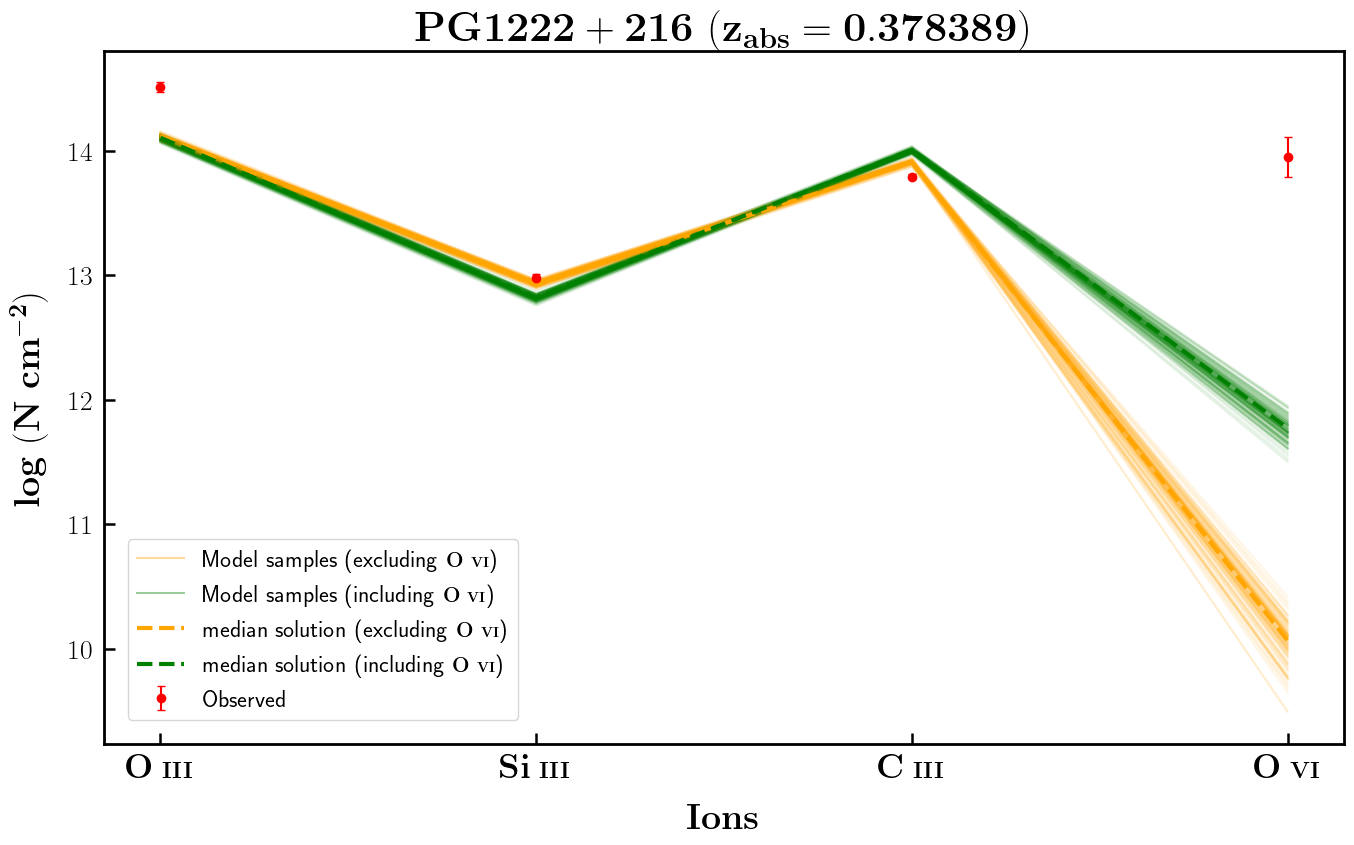
\includegraphics[width=0.9\linewidth]{Ionisation-Modelling-Plots/pg1222-z=0.378389-compVI.png}
    \caption{$\log \text{N}(\ion{H}{i}) \ [\text{cm}^{-2}]=$ 15.43}
  \end{figure}
  
  
  \newpage
  \thispagestyle{empty}

  \begin{landscape}
  
  \begin{figure}
      \centering
      \vspace{-10mm}
      \hspace*{-20mm}
      \captionsetup{oneside,margin={0cm,20mm}}
      \includegraphics[width=1.1\linewidth]{System-Plots/PG1116+215_z=0.138527_sys_plot.png}
      \caption{System plot for the absorber along the LOS of PG 1116+215 at $z_{abs} = 0.138527$. }
  \end{figure}
  
  \end{landscape}
  
  \newgeometry{top=20mm,bottom=0.1cm}
  
  \begin{center} 
  
  \begin{tabular}{cccc} 
  
      \hline \hline \tabularnewline 
      \head{Ion} & \head{v (km s\textsuperscript{$\mathbf{-1}$})} & \head{b (km s\textsuperscript{$\mathbf{-1}$})} & \head{log [N cm\textsuperscript{$\mathbf{-2}$}]}
      \tabularnewline \tabularnewline \hline \tabularnewline 
   
      \ion{N}{v}   &    -7 $\pm$ 3    &    12 $\pm$ 6    &     12.84 $\pm$ 0.09 \\
      \ion{N}{ii}   &    -5 $\pm$ 1    &    6 $\pm$ 3    &     13.62 $\pm$ 0.11 \\
      \ion{N}{ii}   &    33 $\pm$ 6    &    8 $\pm$ 13    &     12.85 $\pm$ 0.15 \\
      \ion{P}{ii}   &    -44 $\pm$ 5    &    19 $\pm$ 8    &     12.94 $\pm$ 0.09 \\
      \ion{Si}{ii}   &    -13 $\pm$ 1    &    9 $\pm$ 1    &     12.46 $\pm$ 0.06 \\
      \ion{Si}{ii}   &    13 $\pm$ 1    &    23 $\pm$ 3    &     12.31 $\pm$ 0.04 \\
      \ion{Si}{iii}   &    -9 $\pm$ 1    &    10 $\pm$ 1    &     12.92 $\pm$ 0.04 \\
      \ion{Si}{iv}   &    -13 $\pm$ 2    &    4 $\pm$ 3    &     12.84 $\pm$ 0.09 \\
      \ion{O}{vi}   &    -1 $\pm$ 1    &    35 $\pm$ 3    &     13.84 $\pm$ 0.02 \\
      \ion{C}{iv}   &    -10 $\pm$ 3    &    13 $\pm$ 4    &     13.17 $\pm$ 0.07 \\
      \ion{C}{ii}   &    -7 $\pm$ 1    &    9 $\pm$ 1    &     13.85 $\pm$ 0.04 \\
      \ion{H}{i}   &    -8 $\pm$ 3    &    27 $\pm$ 2    &     14.97 $\pm$ 0.05 \\
      \ion{H}{i}   &    -5 $\pm$ 9    &    71 $\pm$ 14    &     13.6 $\pm$ 0.23 \\
      \ion{H}{i}   &    31 $\pm$ 2    &    6 $\pm$ 2    &     16.04 $\pm$ 1.77 \\
  
      \tabularnewline \hline \hline \tabularnewline 
  
  \end{tabular}
  
  \end{center}
  
  $\log \text{N}(\ion{H}{i}) \ [\text{cm}^{-2}]=$ 13.60   \\ 
  
  Excluding \ion{O}{vi} : $\log n_H \ (\text{cm}^{-3})$ = -3.24 $\pm$ 0.03 \hspace{10mm} $\log \ Z/Z_\odot$ = 1.92 $\pm$ 0.03
  
  Including \ion{O}{vi} : $\log n_H \ (\text{cm}^{-3})$ = -3.88 $\pm$ 0.01 \hspace{10mm} $\log \ Z/Z_\odot$ = 1.87 $\pm$ 0.02 \\
  
  
%   \newpage 
  
  \begin{figure}[!h]
      \centering
      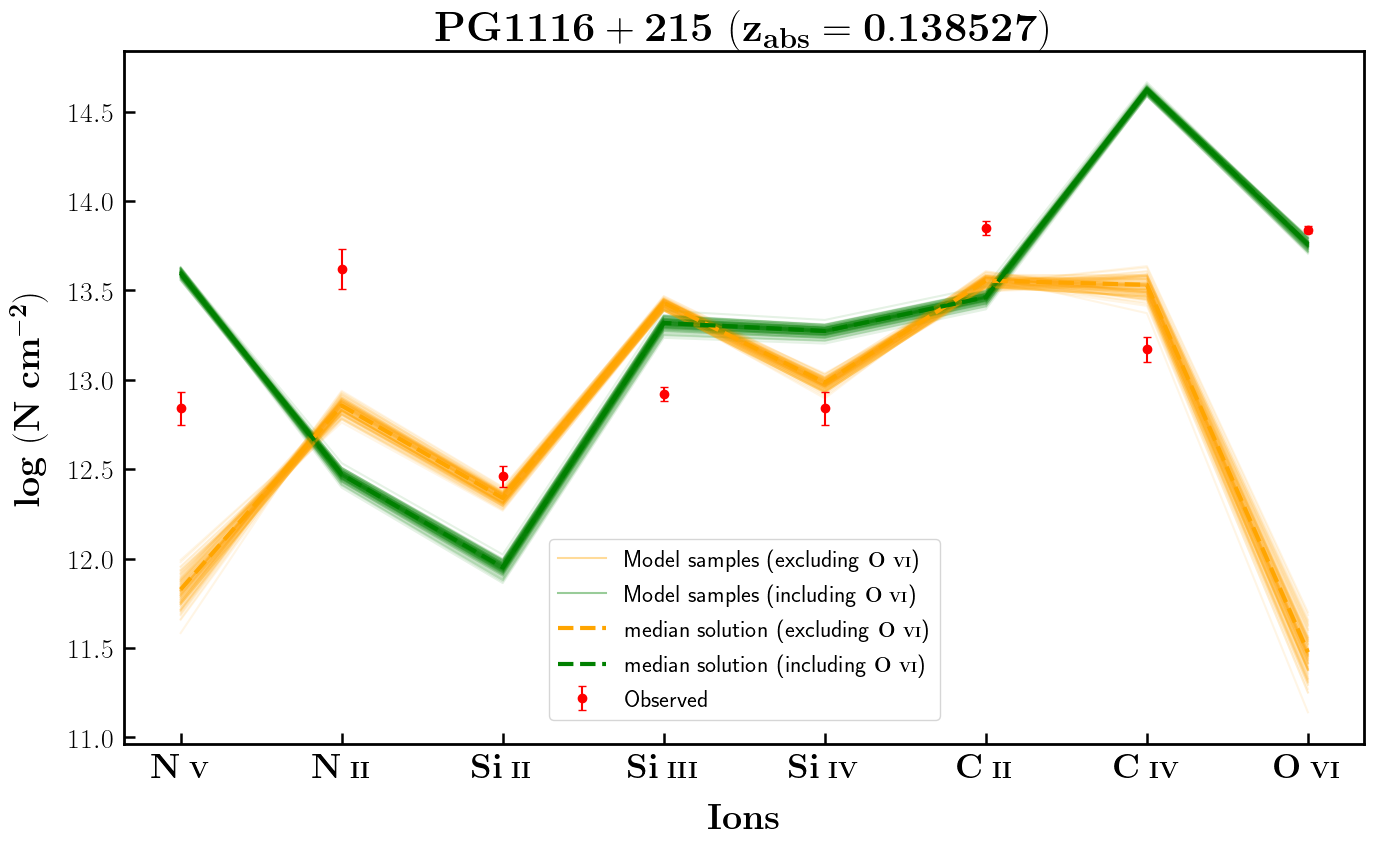
\includegraphics[width=0.9\linewidth]{Ionisation-Modelling-Plots/pg1116-z=0.138527-compII_logZ=-1.png}
      \caption{$\log \text{N}(\ion{H}{i}) \ [\text{cm}^{-2}]=$ 13.60}
  \end{figure}
  
  \restoregeometry
  
  \newpage
  \thispagestyle{empty}

  \begin{landscape}
  
  \begin{figure}
      \centering
      \vspace{-10mm}
      \hspace*{-20mm}
      \captionsetup{oneside,margin={0cm,20mm}}
      \includegraphics[width=1.1\linewidth]{System-Plots/H1821+643_z=0.170006_sys_plot.png}
      \caption{System plot for the absorber along the LOS of H 1821+643 at $z_{abs} = 0.170006$. }
  \end{figure}
  
  \end{landscape}
  
  
  \begin{center} 
  
  \begin{tabular}{cccc} 
  
      \hline \hline \tabularnewline 
      \head{Ion} & \head{v (km s\textsuperscript{$\mathbf{-1}$})} & \head{b (km s\textsuperscript{$\mathbf{-1}$})} & \head{log [N cm\textsuperscript{$\mathbf{-2}$}]}
      \tabularnewline \tabularnewline \hline \tabularnewline 
   
      \ion{Si}{iii}   &    7 $\pm$ 3    &    17 $\pm$ 5    &     12.05 $\pm$ 0.07 \\
      \ion{Si}{iii}   &    52 $\pm$ 6    &    14 $\pm$ 10    &     11.62 $\pm$ 0.17 \\
      \ion{N}{v}   &    47 $\pm$ 3    &    31 $\pm$ 5    &     13.29 $\pm$ 0.05 \\
      \ion{N}{v}   &    122 $\pm$ 7    &    21 $\pm$ 11    &     12.74 $\pm$ 0.14 \\
      \ion{O}{vi}   &    3 $\pm$ 28    &    152 $\pm$ 20    &     13.94 $\pm$ 0.06 \\
      \ion{O}{vi}   &    107 $\pm$ 9    &    48 $\pm$ 12    &     13.29 $\pm$ 0.11 \\
      \ion{H}{i}   &    -92 $\pm$ 1    &    36 $\pm$ 1    &     13.85 $\pm$ 0.02 \\
      \ion{H}{i}   &    0 $\pm$ 2    &    63 $\pm$ 3    &     13.68 $\pm$ 0.02 \\
      \ion{H}{i}   &    120 $\pm$ 1    &    28 $\pm$ 1    &     13.35 $\pm$ 0.02 \\
  
      \tabularnewline \hline \hline \tabularnewline 
  
  \end{tabular}
  
  \end{center}
  
  $\log \text{N}(\ion{H}{i}) \ [\text{cm}^{-2}]=$  13.68  \\ 
  
  Excluding \ion{O}{vi} : $\log n_H \ (\text{cm}^{-3})$ = -4.33 $\pm$ 0.02 \hspace{10mm} $\log \ Z/Z_\odot$ = 1.30 $\pm$ 0.05
  
  Including \ion{O}{vi} : $\log n_H \ (\text{cm}^{-3})$ = -4.43 $\pm$ 0.01 \hspace{10mm} $\log \ Z/Z_\odot$ = 1.25 $\pm$ 0.05
  \\
  
  $\log \text{N}(\ion{H}{i}) \ [\text{cm}^{-2}]=$  13.35  \\ 
  
  Excluding \ion{O}{vi} : $\log n_H \ (\text{cm}^{-3})$ = -4.30 $\pm$ 0.05 \hspace{10mm} $\log \ Z/Z_\odot$ = 1.18 $\pm$ 0.13
  
  Including \ion{O}{vi} : $\log n_H \ (\text{cm}^{-3})$ = -4.41 $\pm$ 0.02 \hspace{10mm} $\log \ Z/Z_\odot$ = 1.15 $\pm$ 0.12
  
  
  \newpage
  
  \begin{figure}[!h]
      \centering
      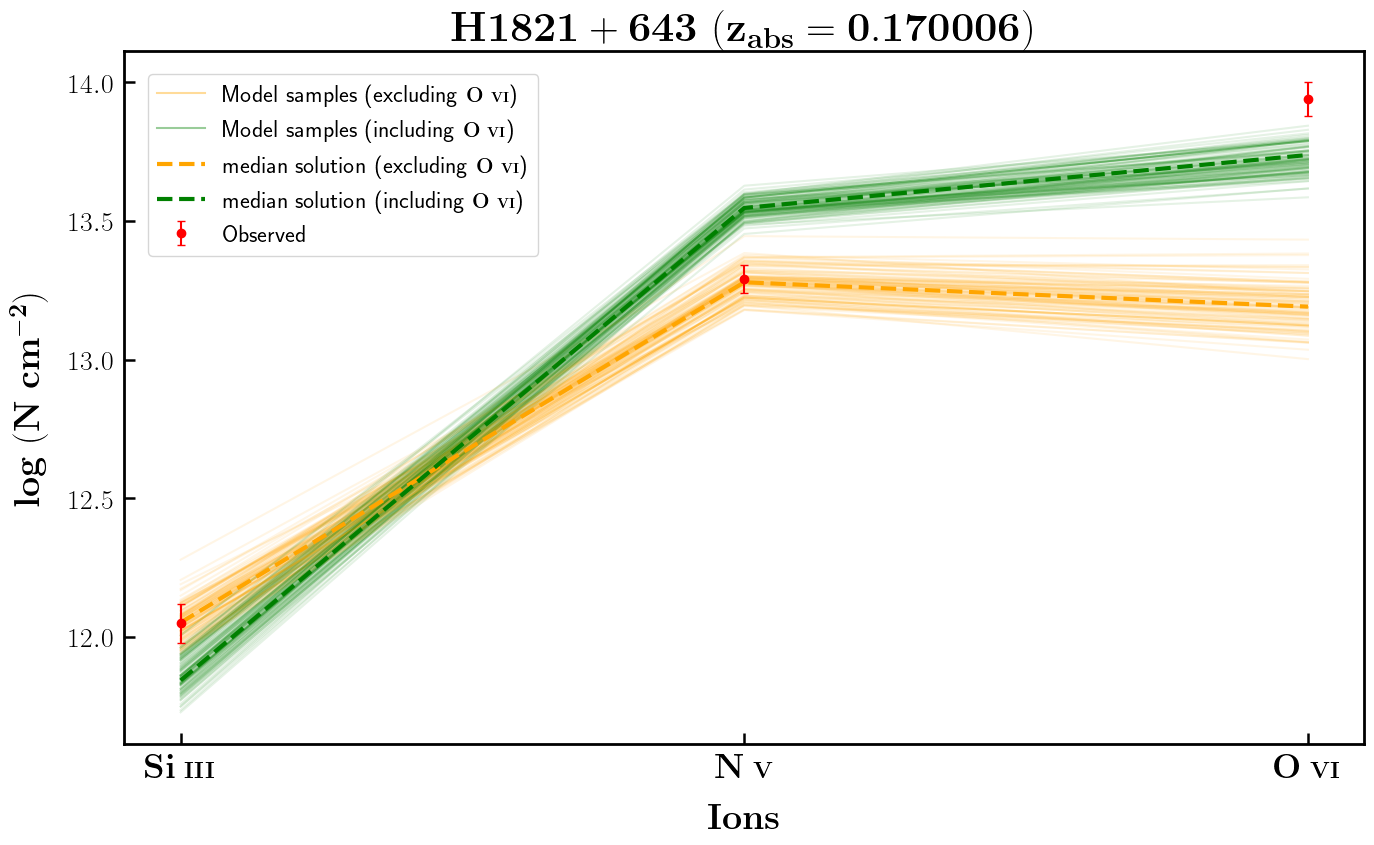
\includegraphics[width=0.9\linewidth]{Ionisation-Modelling-Plots/h1821-z=0.170006-compII.png}
      \caption{$\log \text{N}(\ion{H}{i}) \ [\text{cm}^{-2}]=$ 13.68}
  \end{figure}
  
  \begin{figure}[!b]
      \centering
      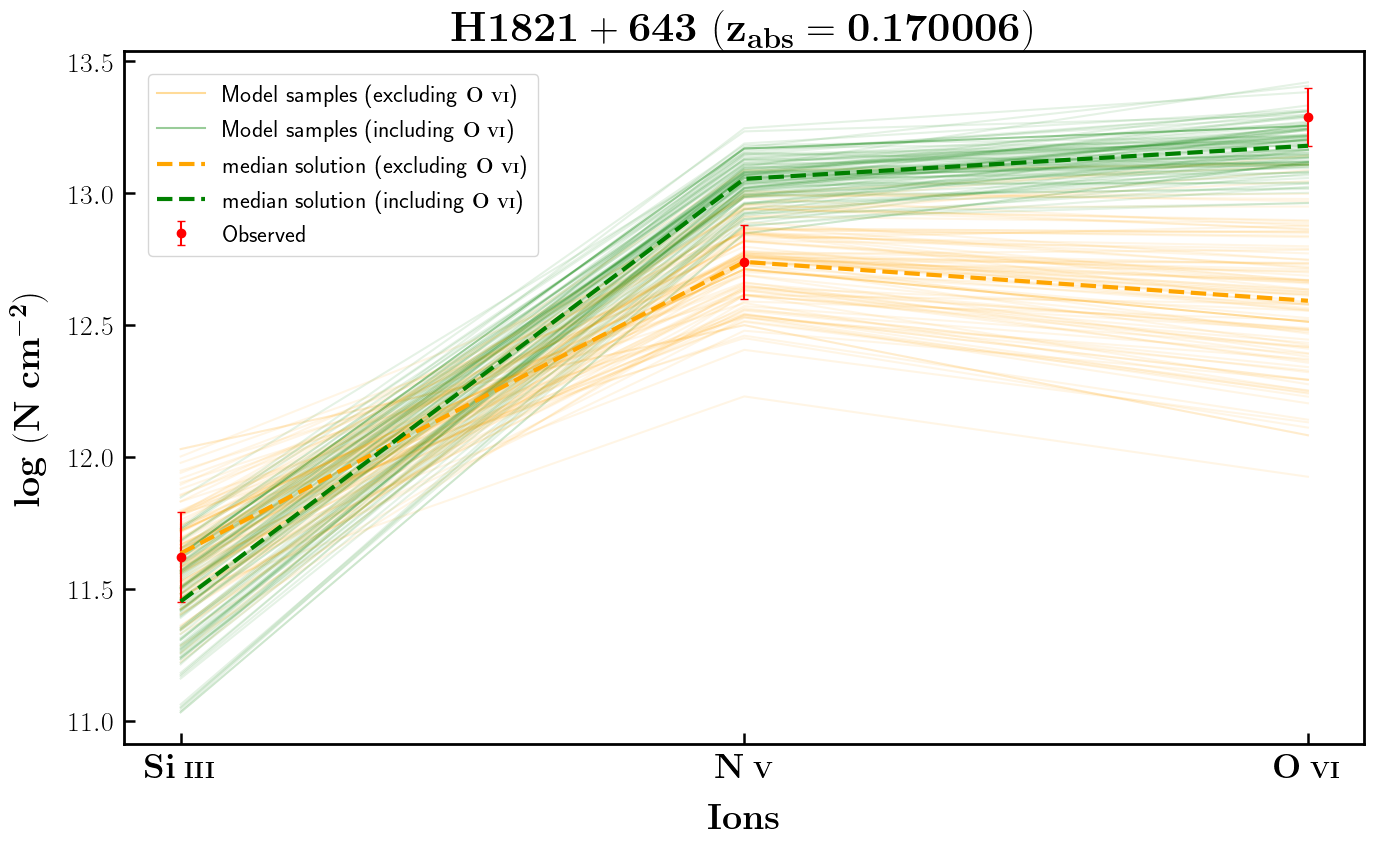
\includegraphics[width=0.9\linewidth]{Ionisation-Modelling-Plots/h1821-z=0.170006-compIII.png}
      \caption{$\log \text{N}(\ion{H}{i}) \ [\text{cm}^{-2}]=$ 13.35}
  \end{figure}
  
  
  \newpage
  \thispagestyle{empty}

  \begin{landscape}
  
  \begin{figure}
      \centering
      \vspace{-10mm}
      \hspace*{-20mm}
      \captionsetup{oneside,margin={0cm,20mm}}
      \includegraphics[width=1.1\linewidth]{System-Plots/H1821+643_z=0.224981_sys_plot.png}
      \caption{System plot for the absorber along the LOS of H 1821+643 at $z_{abs} = 0.224981$. }
  \end{figure}
  
  \end{landscape}
  
  
  \begin{center} 
  
  \begin{tabular}{cccc} 
  
      \hline \hline \tabularnewline 
      \head{Ion} & \head{v (km s\textsuperscript{$\mathbf{-1}$})} & \head{b (km s\textsuperscript{$\mathbf{-1}$})} & \head{log [N cm\textsuperscript{$\mathbf{-2}$}]}
      \tabularnewline \tabularnewline \hline \tabularnewline 
   
      \ion{Si}{iii}   &    -59 $\pm$ 13    &    31 $\pm$ 18    &     12.23 $\pm$ 0.15 \\
      \ion{Si}{iii}   &    -1 $\pm$ 6    &    22 $\pm$ 9    &     12.71 $\pm$ 0.13 \\
      \ion{C}{iii}   &    -31 $\pm$ 1    &    24 $\pm$ 2    &     13.36 $\pm$ 0.07 \\
      \ion{C}{iii}   &    12 $\pm$ 1    &    36 $\pm$ 2    &     13.84 $\pm$ 0.02 \\
      \ion{C}{iii}   &    81 $\pm$ 3    &    15 $\pm$ 5    &     12.6 $\pm$ 0.09 \\
      \ion{C}{iii}   &    335 $\pm$ 7    &    20 $\pm$ 10    &     12.13 $\pm$ 0.11 \\
      \ion{O}{vi}   &    0 $\pm$ 1    &    45 $\pm$ 1    &     14.24 $\pm$ 0.01 \\
      \ion{O}{vi}   &    57 $\pm$ 2    &    3 $\pm$ 3    &     13.12 $\pm$ 0.1 \\
      \ion{O}{vi}   &    330 $\pm$ 1    &    13 $\pm$ 2    &     13.42 $\pm$ 0.03 \\
      \ion{H}{i}   &    -109 $\pm$ 3    &    33 $\pm$ 0    &     13.87 $\pm$ 0.09 \\
      \ion{H}{i}   &    -38 $\pm$ 1    &    30 $\pm$ 1    &     15.16 $\pm$ 0.02 \\
      \ion{H}{i}   &    -19 $\pm$ 10   &    84 $\pm$ 13    &     13.64 $\pm$ 0.11 \\
      \ion{H}{i}   &    18 $\pm$ 1    &    19 $\pm$ 1    &     15.13 $\pm$ 0.03 \\
      \ion{H}{i}   &    276 $\pm$ 7    &    62 $\pm$ 11    &     13.48 $\pm$ 0.06 \\
      
      \tabularnewline \hline \hline \tabularnewline 
  
  \end{tabular}
  
  \end{center}
  
  
  $\log \text{N}(\ion{H}{i}) \ [\text{cm}^{-2}]=$  15.16  \\ 
  
  Excluding \ion{O}{vi} : $\log n_H \ (\text{cm}^{-3})$ = -3.29 $\pm$ 0.08 \hspace{10mm} $\log \ Z/Z_\odot$ = -0.95 $\pm$ 0.07
  
  Including \ion{O}{vi} : $\log n_H \ (\text{cm}^{-3})$ = -4.36 $\pm$ 0.02 \hspace{10mm} $\log \ Z/Z_\odot$ = -0.81 $\pm$ 0.04 \\
  
  $\log \text{N}(\ion{H}{i}) \ [\text{cm}^{-2}]=$  15.13  \\ 
  
  Excluding \ion{O}{vi} : $\log n_H \ (\text{cm}^{-3})$ = -3.29 $\pm$ 0.03 \hspace{10mm} $\log \ Z/Z_\odot$ = -0.44 $\pm$ 0.03
  
  Including \ion{O}{vi} : $\log n_H \ (\text{cm}^{-3})$ = -3.83 $\pm$ 0.04 \hspace{10mm} $\log \ Z/Z_\odot$ = -0.77 $\pm$ 0.03 
  
  \newpage
  
  \begin{figure}[!h]
      \centering
      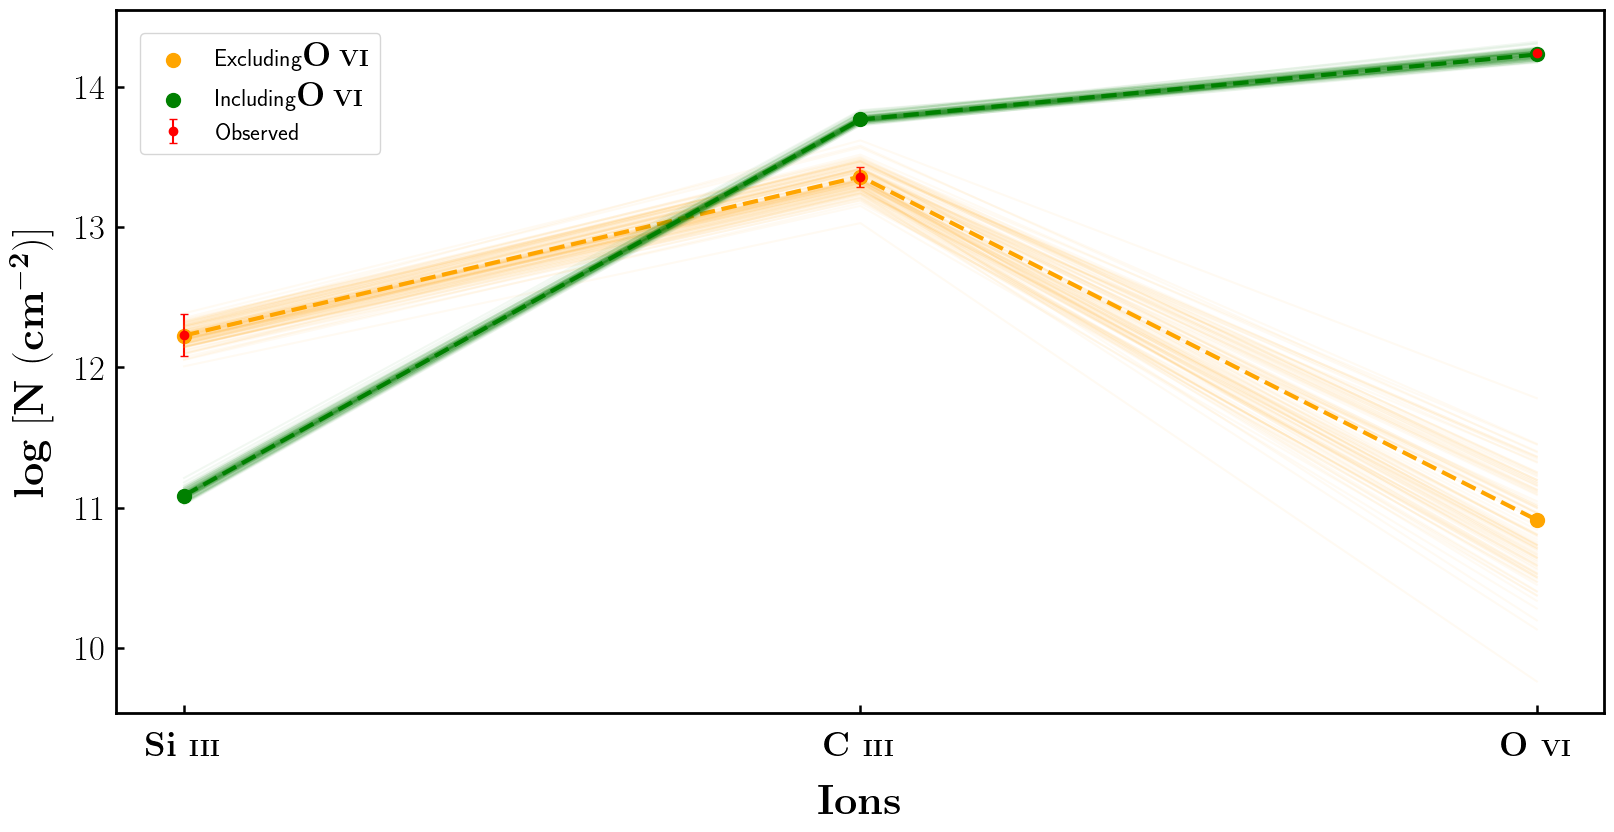
\includegraphics[width=0.9\linewidth]{Ionisation-Modelling-Plots/h1821-z=0.224981-compII.png}
      \caption{$\log \text{N}(\ion{H}{i}) \ [\text{cm}^{-2}]=$ 15.16}
  \end{figure}
  
  \begin{figure}[!b]
      \centering
      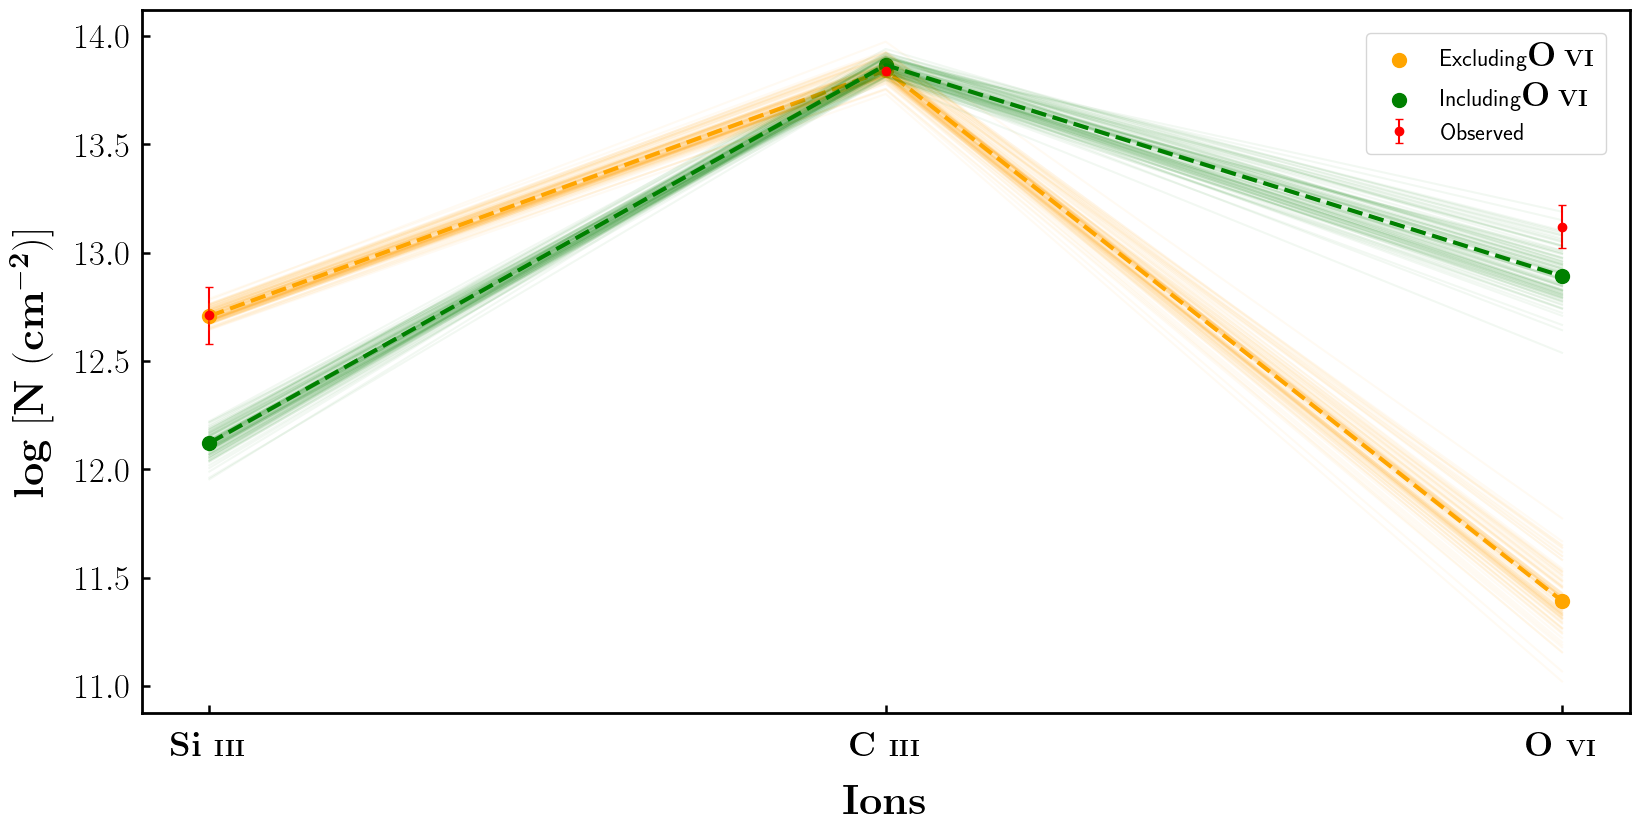
\includegraphics[width=0.9\linewidth]{Ionisation-Modelling-Plots/h1821-z=0.224981-compIV.png}
      \caption{$\log \text{N}(\ion{H}{i}) \ [\text{cm}^{-2}]=$ 15.13}
  \end{figure}
  
  
  
  \newpage
  \thispagestyle{empty}

  \begin{landscape}
  
  \begin{figure}
      \centering
      \vspace{-10mm}
      \hspace*{-20mm}
      \captionsetup{oneside,margin={0cm,20mm}}
      \includegraphics[width=1.1\linewidth]{System-Plots/PG1121+422_z=0.192393_sys_plot.png}
      \caption{System plot for the absorber along the LOS of PG 1121+422 at $z_{abs} = 0.192393$. }
  \end{figure}
  
  \end{landscape}
  
  
  \begin{center} 
  
  \begin{tabular}{cccc} 
  
      \hline \hline \tabularnewline 
      \head{Ion} & \head{v (km s\textsuperscript{$\mathbf{-1}$})} & \head{b (km s\textsuperscript{$\mathbf{-1}$})} & \head{log [N cm\textsuperscript{$\mathbf{-2}$}]}
      \tabularnewline \tabularnewline \hline \tabularnewline 
   
      \ion{Si}{iii}   &    -11 $\pm$ 13    &    10 $\pm$ 3    &     12.62 $\pm$ 0.10 \\
      \ion{Si}{iii}   &    9 $\pm$ 13    &    18 $\pm$ 4    &     13.14 $\pm$ 0.04 \\
      \ion{C}{iii}   &    -26 $\pm$ 10    &    10 $\pm$ 7    &     13.04 $\pm$ 0.09 \\
      \ion{C}{iii}   &    8 $\pm$ 5    &    18 $\pm$ 6    &     13.74 $\pm$ 0.11 \\
      \ion{C}{ii}   &    -9 $\pm$ 3    &    17 $\pm$ 5    &     13.69 $\pm$ 0.08 \\
      \ion{C}{ii}   &    9 $\pm$ 2    &    16 $\pm$ 3    &     13.93 $\pm$ 0.05 \\
      \ion{Si}{iv}   &    10 $\pm$ 7    &    22 $\pm$ 11    &     12.86 $\pm$ 0.13 \\
      \ion{Si}{ii}   &    -3 $\pm$ 1    &    15 $\pm$ 2    &     13.04 $\pm$ 0.06 \\
      \ion{Si}{ii}   &    27 $\pm$ 19    &    42 $\pm$ 1    &     12.48 $\pm$ 0.23 \\
      \ion{O}{vi}   &    -7 $\pm$ 13    &    11 $\pm$ 16    &     12.84 $\pm$ 0.19 \\
      \ion{O}{vi}   &    20 $\pm$ 3    &    3 $\pm$ 4    &     13.37 $\pm$ 0.12 \\
      \ion{H}{i}   &    1 $\pm$ 2    &    60 $\pm$ 6    &     14.34 $\pm$ 0.09 \\
      \ion{H}{i}   &    5 $\pm$ 1    &    19 $\pm$ 1    &     17.7 $\pm$ 0.11 \\
  
      \tabularnewline \hline \hline \tabularnewline 
  
  \end{tabular}
  
  \end{center}
  
  
  $\log \text{N}(\ion{H}{i}) \ [\text{cm}^{-2}]=$ 14.34   \\ 
  
  Excluding \ion{O}{vi} : $\log n_H \ (\text{cm}^{-3})$ = -1.78 $\pm$ 0.05 \hspace{10mm} $\log \ Z/Z_\odot$ = 1.97 $\pm$ 0.04
  
  Including \ion{O}{vi} : $\log n_H \ (\text{cm}^{-3})$ = -3.00 $\pm$ 0.04 \hspace{10mm} $\log \ Z/Z_\odot$ = 1.25 $\pm$ 0.04 \\
  
  $\log \text{N}(\ion{H}{i}) \ [\text{cm}^{-2}]=$  17.70  
  
  Excluding \ion{O}{vi} : $\log n_H \ (\text{cm}^{-3})$ = -2.35 $\pm$ 0.05 \hspace{10mm} $\log \ Z/Z_\odot$ = -1.66 $\pm$ 0.06
  
  Including \ion{O}{vi} : $\log n_H \ (\text{cm}^{-3})$ = -3.08 $\pm$ 0.04 \hspace{10mm} $\log \ Z/Z_\odot$ = -2.08 $\pm$ 0.05 
  
  
  \newpage
  
  \begin{figure}[!h]
      \centering
      \includegraphics[width=0.9\linewidth]{Ionisation-Modelling-Plots/pg1121-z=0.192393-compI_logZ=-1.png}
      \caption{$\log \text{N}(\ion{H}{i}) \ [\text{cm}^{-2}]=$ 14.34}
  \end{figure}
  
  \begin{figure}[!b]
    \centering
    \includegraphics[width=0.9\linewidth]{Ionisation-Modelling-Plots/pg1121-z=0.192393-compII.png}
    \caption{$\log \text{N}(\ion{H}{i}) \ [\text{cm}^{-2}]=$ 17.70}
  \end{figure}
  
  
  
  \newpage
  \thispagestyle{empty}

  \begin{landscape}
  
  \begin{figure}
      \centering
      \vspace{-10mm}
      \hspace*{-20mm}
      \captionsetup{oneside,margin={0cm,20mm}}
      \includegraphics[width=1.1\linewidth]{System-Plots/PKS0405-123_z=0.167125_sys_plot.png}
      \caption{System plot for the absorber along the LOS of PKS 0405-123 at $z_{abs} = 0.167125$. }
  \end{figure}
  
  \end{landscape}

  \newgeometry{top=30mm,bottom=0.1cm}
  
  \begin{center} 
    
%    \begin{table}[H]
%     \centering

  \begin{tabular}{cccc}
  
      \hline \hline \tabularnewline 
      \head{Ion} & \head{v (km s\textsuperscript{$\mathbf{-1}$})} & \head{b (km s\textsuperscript{$\mathbf{-1}$})} & \head{log [N cm\textsuperscript{$\mathbf{-2}$}]}
      \tabularnewline \tabularnewline \hline \tabularnewline 
   
      \ion{O}{i}   &    -14 $\pm$ 5    &    23 $\pm$ 7    &     13.52 $\pm$ 0.08 \\
      \ion{C}{ii}   &    -37 $\pm$ 2    &    16 $\pm$ 2    &     13.76 $\pm$ 0.02 \\
      \ion{C}{ii}   &    -1 $\pm$ 1    &    6 $\pm$ 1    &     16.27 $\pm$ 0.12 \\
      \ion{C}{iii}   &    -136 $\pm$ 2    &    32 $\pm$ 2    &     13.45 $\pm$ 0.02 \\
      \ion{C}{iii}   &    -26 $\pm$ 0    &    37 $\pm$ 2    &     14.33 $\pm$ 0.04 \\
      \ion{N}{ii}   &    -27 $\pm$ 6    &    44 $\pm$ 5    &     13.47 $\pm$ 0.09 \\
      \ion{N}{ii}   &    -7 $\pm$ 1    &    12 $\pm$ 1    &     14.11 $\pm$ 0.02 \\
      \ion{N}{iii}   &    -7 $\pm$ 0    &    9 $\pm$ 4    &     14.06 $\pm$ 0.08 \\
      \ion{N}{iii}   &    5 $\pm$ 0    &    50 $\pm$ 2    &     14.43 $\pm$ 0.02 \\
      \ion{N}{v}   &    -276 $\pm$ 3    &    30 $\pm$ 0    &     13.25 $\pm$ 0.05 \\
      \ion{N}{v}   &    -116 $\pm$ 0    &    59 $\pm$ 9    &     13.32 $\pm$ 0.08 \\
      \ion{N}{v}   &    -79 $\pm$ 13    &    24 $\pm$ 12    &     12.77 $\pm$ 0.19 \\
      \ion{N}{v}   &    -3 $\pm$ 2    &    43 $\pm$ 3    &     13.89 $\pm$ 0.03 \\
      \ion{Si}{iii}   &    -41 $\pm$ 3    &    13 $\pm$ 4    &     12.66 $\pm$ 0.10 \\
      \ion{Si}{iii}   &    -1 $\pm$ 2    &    22 $\pm$ 2    &     13.28 $\pm$ 0.03 \\
      \ion{Si}{iv}   &    -128 $\pm$ 0    &    25 $\pm$ 5    &     12.61 $\pm$ 0.06 \\
      \ion{Si}{iv}   &    2 $\pm$ 1    &    31 $\pm$ 2    &     13.25 $\pm$ 0.02 \\
      \ion{Si}{ii}   &    -48 $\pm$ 5    &    26 $\pm$ 8    &     12.54 $\pm$ 0.09 \\
      \ion{Si}{ii}   &    -4 $\pm$ 1    &    15 $\pm$ 0    &     13.24 $\pm$ 0.02 \\
      \ion{O}{vi}   &    -268 $\pm$ 0    &    74 $\pm$ 5    &     14.05 $\pm$ 0.02 \\
      \ion{O}{vi}   &    -129 $\pm$ 8    &    41 $\pm$ 3    &     14.05 $\pm$ 0.10 \\
      \ion{O}{vi}   &    -64 $\pm$ 5    &    32 $\pm$ 2    &     14.11 $\pm$ 0.17 \\
      \ion{O}{vi}   &    -2 $\pm$ 4    &    43 $\pm$ 3    &     14.49 $\pm$ 0.05 \\
      \ion{H}{i}   &    -158 $\pm$ 0    &    56 $\pm$ 9    &     13.09 $\pm$ 0.06 \\
      \ion{H}{i}   &    -127 $\pm$ 4    &    26 $\pm$ 3    &     13.46 $\pm$ 0.04 \\
      \ion{H}{i}   &    -80 $\pm$ 1    &    18 $\pm$ 2    &     13.54 $\pm$ 0.04 \\
      \ion{H}{i}   &    -30 $\pm$ 0    &    18 $\pm$ 2    &     15.98 $\pm$ 0.34 \\
      \ion{H}{i}   &    8 $\pm$ 49    &    19 $\pm$ 0    &     17.53 $\pm$ 0.07 \\
      \ion{H}{i}   &    54 $\pm$ 90    &    30 $\pm$ 2    &     13.66 $\pm$ 0.04 \\
      
      \tabularnewline \hline \hline 
  
  \end{tabular}
% \end{table} 
  
  \end{center}

  \restoregeometry
  
  $\log \text{N}(\ion{H}{i}) \ [\text{cm}^{-2}]=$  13.46  \\ 
  
  Excluding \ion{O}{vi} : $\log n_H \ (\text{cm}^{-3})$ = -3.98 $\pm$ 0.03 \hspace{10mm} $\log \ Z/Z_\odot$ = 0.62 $\pm$ 0.02
  
  Including \ion{O}{vi} : $\log n_H \ (\text{cm}^{-3})$ = -4.17 $\pm$ 0.02 \hspace{10mm} $\log \ Z/Z_\odot$ = 0.63 $\pm$ 0.02
  \\\\
  
  $\log \text{N}(\ion{H}{i}) \ [\text{cm}^{-2}]=$  15.98  \\ 
  
  Excluding \ion{O}{vi} : $\log n_H \ (\text{cm}^{-3})$ = -2.73 $\pm$ 0.04 \hspace{10mm} $\log \ Z/Z_\odot$ = -0.18 $\pm$ 0.02
  
  Including \ion{O}{vi} : $\log n_H \ (\text{cm}^{-3})$ = -3.27 $\pm$ 0.03 \hspace{10mm} $\log \ Z/Z_\odot$ = -0.33 $\pm$ 0.02
  \\\\
  
  \begin{figure}[!h]
    \centering
    \includegraphics[width=0.9\linewidth]{Ionisation-Modelling-Plots/pks0405-z=0.167125-compII.png}
    \caption{$\log \text{N}(\ion{H}{i}) \ [\text{cm}^{-2}]=$ 13.46}
  \end{figure}
  
  
  \newpage
  
  \begin{figure}[!h]
    \centering
    \includegraphics[width=0.9\linewidth]{Ionisation-Modelling-Plots/pks0405-z=0.167125-compIV.png}
    \caption{$\log \text{N}(\ion{H}{i}) \ [\text{cm}^{-2}]=$ 15.98}
  \end{figure}
  
  
  \newpage
  \thispagestyle{empty}

  \begin{landscape}
  
  \begin{figure}
      \centering
      \vspace{-10mm}
      \hspace*{-20mm}
      \captionsetup{oneside,margin={0cm,20mm}}
      \includegraphics[width=1.1\linewidth]{System-Plots/HE0056-3622_z=0.043265_sys_plot.png}
      \caption{System plot for the absorber along the LOS of HE 0056-3622 at $z_{abs} = 0.043265$. }
  \end{figure}
  
  \end{landscape}
  
  
  \begin{center} 
  
  \begin{tabular}{cccc} 
  
      \hline \hline \tabularnewline 
      \head{Ion} & \head{v (km s\textsuperscript{$\mathbf{-1}$})} & \head{b (km s\textsuperscript{$\mathbf{-1}$})} & \head{log [N cm\textsuperscript{$\mathbf{-2}$}]}
      \tabularnewline \tabularnewline \hline \tabularnewline 
   
      \ion{Si}{iii}   &    27 $\pm$ 6   &    34 $\pm$ 9    &     12.37 $\pm$ 0.07 \\
      \ion{N}{v}   &    -26 $\pm$ 4   &    1 $\pm$ 8    &     13.42 $\pm$ 0.46 \\
      \ion{C}{iv}   &    30 $\pm$ 2   &    31 $\pm$ 0    &     13.64 $\pm$ 0.03 \\
      \ion{H}{i}   &    0 $\pm$ 3   &    85 $\pm$ 6    &     14.02 $\pm$ 0.07 \\
      \ion{H}{i}   &    12 $\pm$ 1   &    32 $\pm$ 4    &     15.3 $\pm$ 0.1 \\
  
      \tabularnewline \hline \hline \tabularnewline 
  
  \end{tabular}
  
  \end{center}
  
  $\log \text{N}(\ion{H}{i}) \ [\text{cm}^{-2}]=$  15.30  \\ \hspace*{4mm}
  Solution : $\log n_H \ (\text{cm}^{-3})$ = -4.03 $\pm$ 0.03 \hspace{10mm} $\log \ Z/Z_\odot$ = -0.78 $\pm$ 0.04 \\ 
  
  \begin{figure}[!h]
    \centering
    \includegraphics[width=0.9\linewidth]{Ionisation-Modelling-Plots/he0056-z=0.043265-compII_logZ=-1.png}
    \caption{$\log \text{N}(\ion{H}{i}) \ [\text{cm}^{-2}]=$ 15.30}
  \end{figure}
  
  
  \newpage
  \thispagestyle{empty}

  \begin{landscape}
  
  \begin{figure}
      \centering
      \vspace{-10mm}
      \hspace*{-20mm}
      \captionsetup{oneside,margin={0cm,20mm}}
      \includegraphics[width=1.1\linewidth]{System-Plots/PG1216+069_z=0.006328_sys_plot.png}
      \caption{System plot for the absorber along the LOS of PG 1216+069 at $z_{abs} = 0.006328$. }
  \end{figure}
  
  \end{landscape}
  
  \newgeometry{bottom=0.1cm}

  \begin{center} 
  
  \begin{tabular}{cccc} 
  
      \hline \hline \tabularnewline 
      \head{Ion} & \head{v (km s\textsuperscript{$\mathbf{-1}$})} & \head{b (km s\textsuperscript{$\mathbf{-1}$})} & \head{log [N cm\textsuperscript{$\mathbf{-2}$}]}
      \tabularnewline \tabularnewline \hline \tabularnewline 
   
      \ion{O}{i}   &    8 $\pm$ 2   &    7 $\pm$ 5    &     14.07 $\pm$ 0.16 \\
      \ion{O}{i}   &    25 $\pm$ 12   &    50 $\pm$ 13    &     14.0 $\pm$ 0.11 \\
      \ion{C}{ii}   &    0 $\pm$ 3   &    7 $\pm$ 5    &     13.98 $\pm$ 0.08 \\
      \ion{C}{ii}   &    24 $\pm$ 19   &    17 $\pm$ 6    &     13.43 $\pm$ 0.09 \\
      \ion{Si}{ii}   &    -68 $\pm$ 4   &    21 $\pm$ 6    &     12.51 $\pm$ 0.06 \\
      \ion{Si}{ii}   &    6 $\pm$ 1   &    18 $\pm$ 0    &     13.2 $\pm$ 0.02 \\
      \ion{H}{i}   &    -233 $\pm$ 110   &    95 $\pm$ 15    &     13.56 $\pm$ 0.06 \\
      \ion{H}{i}   &    -68 $\pm$ 0   &    81 $\pm$ 8    &     14.76 $\pm$ 0.12 \\
      \ion{H}{i}   &    0 $\pm$ 0   &    106 $\pm$ 15    &     14.79 $\pm$ 0.08 \\
      \ion{H}{i}   &    24 $\pm$ 0   &    20 $\pm$ 12    &     19.09 $\pm$ 0.03 \\
  
      \tabularnewline \hline \hline \tabularnewline 
  
  \end{tabular}
  
  \end{center}
  
  
  $\log \text{N}(\ion{H}{i}) \ [\text{cm}^{-2}]$ = 14.79   \\ \hspace*{4mm}
  Solution : $\log n_H \ (\text{cm}^{-3})$ = -2.69 $\pm$ 0.05 \hspace{10mm} $\log \ Z/Z_\odot$ = 1.97 $\pm$ 0.04 \\ 
  
%   \newpage
  
  \begin{figure}[!h]
    \centering
    \includegraphics[width=0.9\linewidth]{Ionisation-Modelling-Plots/pg1216-z=0.006328-compIII_logZ=1.png}
    \caption{$\log \text{N}(\ion{H}{i}) \ [\text{cm}^{-2}]=$ 14.79}
  \end{figure}
  
  \restoregeometry
  
  \newpage
  \thispagestyle{empty}

  \begin{landscape}
  
  \begin{figure}
      \centering
      \vspace{-10mm}
      \hspace*{-20mm}
      \captionsetup{oneside,margin={0cm,20mm}}
      \includegraphics[width=1.1\linewidth]{System-Plots/3C263_z=0.063397_sys_plot.png}
      \caption{System plot for the absorber along the LOS of 3C 263 at $z_{abs} = 0.063397$. }
  \end{figure}
  
  \end{landscape}
  
  \newgeometry{bottom=0.1cm}
  
  \begin{center} 
  
  \begin{tabular}{cccc} 
  
      \hline \hline \tabularnewline 
      \head{Ion} & \head{v (km s\textsuperscript{$\mathbf{-1}$})} & \head{b (km s\textsuperscript{$\mathbf{-1}$})} & \head{log [N cm\textsuperscript{$\mathbf{-2}$}]}
      \tabularnewline \tabularnewline \hline \tabularnewline 
   
      \ion{Si}{ii}   &    26 $\pm$ 2   &    8 $\pm$ 4    &     12.29 $\pm$ 0.06 \\
      \ion{Si}{iii}   &    -39 $\pm$ 1   &    21 $\pm$ 2    &     12.64 $\pm$ 0.03 \\
      \ion{Si}{iii}   &    34 $\pm$ 1   &    12 $\pm$ 1    &     12.91 $\pm$ 0.04 \\
      \ion{Si}{iv}   &    25 $\pm$ 1   &    22 $\pm$ 0    &     13.57 $\pm$ 0.02 \\
      \ion{C}{iv}   &    -35 $\pm$ 1   &    12 $\pm$ 3    &     13.42 $\pm$ 0.06 \\
      \ion{C}{iv}   &    0 $\pm$ 2   &    13 $\pm$ 3    &     13.63 $\pm$ 0.06 \\
      \ion{C}{iv}   &    38 $\pm$ 2   &    17 $\pm$ 2    &     13.86 $\pm$ 0.04 \\
      \ion{C}{ii}   &    34 $\pm$ 2   &    17 $\pm$ 3    &     13.37 $\pm$ 0.04 \\
      \ion{H}{i}   &    -146 $\pm$ 2   &    25 $\pm$ 2    &     13.87 $\pm$ 0.04 \\
      \ion{H}{i}   &    -35 $\pm$ 0   &    50 $\pm$ 6    &     14.88 $\pm$ 0.12 \\
      \ion{H}{i}   &    0 $\pm$ 0   &    54 $\pm$ 6    &     14.42 $\pm$ 0.2 \\
      \ion{H}{i}   &    38 $\pm$ 0   &    12 $\pm$ 3    &     16.46 $\pm$ 0.13 \\
  
      \tabularnewline \hline \hline \tabularnewline 
  
  \end{tabular}
  
  \end{center}
  
  
  $\log \text{N}(\ion{H}{i}) \ [\text{cm}^{-2}]$ = 16.46   \\  \hspace*{4mm}
  Solution : $\log n_H \ (\text{cm}^{-3})$ = -3.72 $\pm$ 0.02 \hspace{10mm} $\log \ Z/Z_\odot$ = -0.99 $\pm$ 0.02 \\  
  
%   \newpage 
  
  \begin{figure}[!h]
      \centering
    %   \vspace*{-10mm}
      \includegraphics[width=0.9\linewidth]{Ionisation-Modelling-Plots/3c263-z=0.063397-compIV_logZ=-1.png}
      \caption{$\log \text{N}(\ion{H}{i}) \ [\text{cm}^{-2}]=$ 16.46}
  \end{figure}
  
  \restoregeometry
  
  \newpage
  \thispagestyle{empty}

  \begin{landscape}
  
  \begin{figure}
      \centering
      \vspace{-10mm}
      \hspace*{-20mm}
      \captionsetup{oneside,margin={0cm,20mm}}
      \includegraphics[width=1.1\linewidth]{System-Plots/PG1222+216_z=0.054479_sys_plot.png}
      \caption{System plot for the absorber along the LOS of PG 1222+216 at $z_{abs} = 0.054479$. }
  \end{figure}
  
  \end{landscape}
  
  
  \begin{center} 
  
  \begin{tabular}{cccc} 
  
      \hline \hline \tabularnewline 
      \head{Ion} & \head{v (km s\textsuperscript{$\mathbf{-1}$})} & \head{b (km s\textsuperscript{$\mathbf{-1}$})} & \head{log [N cm\textsuperscript{$\mathbf{-2}$}]}
      \tabularnewline \tabularnewline \hline \tabularnewline 
   
      \ion{Si}{iii}   &    -12 $\pm$ 3   &    20 $\pm$ 3    &     13.19 $\pm$ 0.05 \\
      \ion{Si}{iii}   &    40 $\pm$ 5   &    27 $\pm$ 5    &     13.04 $\pm$ 0.07 \\
      \ion{Si}{iv}   &    0 $\pm$ 1   &    25 $\pm$ 8    &     12.89 $\pm$ 0.08 \\
      \ion{Si}{iv}   &    41 $\pm$ 4   &    10 $\pm$ 7    &     12.39 $\pm$ 0.13 \\
      \ion{C}{iv}   &    -2 $\pm$ 1   &    29 $\pm$ 6    &     13.55 $\pm$ 0.1 \\
      \ion{C}{iv}   &    41 $\pm$ 8   &    34 $\pm$ 6    &     13.5 $\pm$ 0.11 \\
      \ion{C}{iv}   &    182 $\pm$ 10   &    26 $\pm$ 15    &     12.86 $\pm$ 0.15 \\
      \ion{C}{ii}   &    7 $\pm$ 4   &    26 $\pm$ 6    &     13.51 $\pm$ 0.07 \\
      \ion{C}{ii}   &    51 $\pm$ 4   &    10 $\pm$ 6    &     12.98 $\pm$ 0.09 \\
      \ion{H}{i}   &    -12 $\pm$ 23   &    74 $\pm$ 11    &     14.08 $\pm$ 0.15 \\
      \ion{H}{i}   &    5 $\pm$ 4   &    24 $\pm$ 3    &     17.91 $\pm$ 0.15 \\
  
      \tabularnewline \hline \hline \tabularnewline 
  
  \end{tabular}
  
  \end{center}
  
  $\log \text{N}(\ion{H}{i}) \ [\text{cm}^{-2}]$ = 14.08 \\ \hspace*{4mm}
  Solution : $\log n_H \ (\text{cm}^{-3})$ = -3.45 $\pm$ 0.06 \hspace{10mm} $\log \ Z/Z_\odot$ = 1.25 $\pm$ 0.05 \\  
  
  $\log \text{N}(\ion{H}{i}) \ [\text{cm}^{-2}]$ = 17.91   \\  \hspace*{4mm}
  Solution : $\log n_H \ (\text{cm}^{-3})$ = -3.86 $\pm$ 0.08 \hspace{10mm} $\log \ Z/Z_\odot$ = -2.91 $\pm$ 0.07 \newline  
  
  \newpage
  
  \begin{figure}[!h]
      \centering
      \includegraphics[width=0.9\linewidth]{Ionisation-Modelling-Plots/pg1222-z=0.054479-compI_logZ=-1.png}
      \caption{$\log \text{N}(\ion{H}{i}) \ [\text{cm}^{-2}]=$ 14.08}
  \end{figure}
  
  \begin{figure}[!b]
      \centering
      \includegraphics[width=0.9\linewidth]{Ionisation-Modelling-Plots/pg1222-z=0.054479-compII_logZ=-1.png}
      \caption{$\log \text{N}(\ion{H}{i}) \ [\text{cm}^{-2}]=$ 17.91}
  \end{figure}
  
  
  \newpage
  \thispagestyle{empty}

  \begin{landscape}
  
  \begin{figure}
      \centering
      \vspace{-10mm}
      \hspace*{-20mm}
      \captionsetup{oneside,margin={0cm,20mm}}
      \includegraphics[width=1.1\linewidth]{System-Plots/RXJ0439.6-5311_z=0.005568_sys_plot.png}
      \caption{System plot for the absorber along the LOS of RX J0439.6-5311 at $z_{abs} = 0.005568$. }
  \end{figure}
  
  \end{landscape}
  
  
  \begin{center} 
  
  \begin{tabular}{cccc} 
  
      \hline \hline \tabularnewline 
      \head{Ion} & \head{v (km s\textsuperscript{$\mathbf{-1}$})} & \head{b (km s\textsuperscript{$\mathbf{-1}$})} & \head{log [N cm\textsuperscript{$\mathbf{-2}$}]}
      \tabularnewline \tabularnewline \hline \tabularnewline 
   
      \ion{Si}{iii}   &    16 $\pm$ 1   &    11 $\pm$ 3    &     13.01 $\pm$ 0.12 \\
      \ion{Si}{iv}   &    -3 $\pm$ 4   &    20 $\pm$ 6    &     12.77 $\pm$ 0.08 \\
      \ion{C}{iv}   &    4 $\pm$ 3   &    13 $\pm$ 5    &     13.5 $\pm$ 0.07 \\
      \ion{H}{i}   &    0 $\pm$ 2   &    53 $\pm$ 6    &     14.3 $\pm$ 0.09 \\
      \ion{H}{i}   &    5 $\pm$ 3   &    15 $\pm$ 6    &     16.11 $\pm$ 0.26 \\
  
      \tabularnewline \hline \hline \tabularnewline 
  
  \end{tabular}
  
  \end{center}
  
  
  $\log \text{N}(\ion{H}{i}) \ [\text{cm}^{-2}]=$  16.11  \\ \hspace*{4mm}
  Solution : $\log n_H \ (\text{cm}^{-3})$ = -3.69 $\pm$ 0.07 \hspace{10mm} $\log \ Z/Z_\odot$ = -1.07 $\pm$ 0.1 \newline
  
  \begin{figure}[!h]
      \centering
      \includegraphics[width=0.9\linewidth]{Ionisation-Modelling-Plots/rxj0439-z=0.005568-compII_logZ=-1.png}
      \caption{$\log \text{N}(\ion{H}{i}) \ [\text{cm}^{-2}]=$ 16.11}
  \end{figure}
  
  
  
  \newpage
  \thispagestyle{empty}

  \begin{landscape}
  
  \begin{figure}
      \centering
      \vspace{-10mm}
      \hspace*{-20mm}
      \captionsetup{oneside,margin={0cm,20mm}}
      \includegraphics[width=1.1\linewidth]{System-Plots/UKS0242-724_z=0.063850_sys_plot.png}
      \caption{System plot for the absorber along the LOS of UKS 0242-724 at $z_{abs} = 0.063850$. }
  \end{figure}
  
  \end{landscape}
  
  \newgeometry{bottom=0.1cm}

  \begin{center} 
  
  \begin{tabular}{cccc} 
  
      \hline \hline \tabularnewline 
      \head{Ion} & \head{v (km s\textsuperscript{$\mathbf{-1}$})} & \head{b (km s\textsuperscript{$\mathbf{-1}$})} & \head{log [N cm\textsuperscript{$\mathbf{-2}$}]}
      \tabularnewline \tabularnewline \hline \tabularnewline 
   
      \ion{Fe}{ii}   &    -90 $\pm$ 4   &    9 $\pm$ 9    &     13.49 $\pm$ 0.14 \\
      \ion{C}{ii}   &    -84 $\pm$ 2   &    7 $\pm$ 5    &     13.46 $\pm$ 0.11 \\
      \ion{C}{ii}   &    0 $\pm$ 3   &    3 $\pm$ 7    &     13.55 $\pm$ 0.16 \\
      \ion{C}{ii}   &    24 $\pm$ 5   &    9 $\pm$ 6    &     13.32 $\pm$ 0.1 \\
      \ion{Si}{ii}   &    -78 $\pm$ 3   &    25 $\pm$ 5    &     12.6 $\pm$ 0.05 \\
      \ion{Si}{ii}   &    10 $\pm$ 2   &    15 $\pm$ 4    &     12.52 $\pm$ 0.06 \\
      \ion{H}{i}   &    -84 $\pm$ 0   &    30 $\pm$ 5    &     14.61 $\pm$ 0.06 \\
      \ion{H}{i}   &    0 $\pm$ 0   &    46 $\pm$ 6    &     15.17 $\pm$ 0.1 \\
      \ion{H}{i}   &    24 $\pm$ 0   &    19 $\pm$ 6    &     15.34 $\pm$ 1.33 \\
  
      \tabularnewline \hline \hline \tabularnewline 
  
  \end{tabular}
  
  \end{center}
  
  
  $\log \text{N}(\ion{H}{i}) \ [\text{cm}^{-2}]$ = 14.61   \\ \hspace*{4mm}
  Solution : $\log n_H \ (\text{cm}^{-3})$ = -2.23 $\pm$ 0.13 \hspace{10mm} $\log \ Z/Z_\odot$ = 1.92 $\pm$ 0.10 \newline 
  
  
  \begin{figure}[!h]
    \centering
    \includegraphics[width=0.9\linewidth]{Ionisation-Modelling-Plots/uks0242-z=0.06385-compI_logZ=1.png}
    \caption{$\log \text{N}(\ion{H}{i}) \ [\text{cm}^{-2}]=$ 14.61}
  \end{figure}
  
  \restoregeometry
  
  \newpage
  \thispagestyle{empty}

  \begin{landscape}
  
  \begin{figure}
      \centering
      \vspace{-10mm}
      \hspace*{-20mm}
      \captionsetup{oneside,margin={0cm,20mm}}
      \includegraphics[width=1.1\linewidth]{System-Plots/PG1259+593_z=0.046284_sys_plot.png}
      \caption{System plot for the absorber along the LOS of PG 1259+593 at $z_{abs} = 0.046284$. }
  \end{figure}
  
  \end{landscape}
  
  \newgeometry{bottom=0.1cm}
  
  \begin{center} 
  
  \begin{tabular}{cccc} 
  
      \hline \hline \tabularnewline 
      \head{Ion} & \head{v (km s\textsuperscript{$\mathbf{-1}$})} & \head{b (km s\textsuperscript{$\mathbf{-1}$})} & \head{log [N cm\textsuperscript{$\mathbf{-2}$}]}
      \tabularnewline \tabularnewline \hline \tabularnewline 
   
      \ion{C}{iv}   &    -34 $\pm$ 2   &    31 $\pm$ 3    &     13.7 $\pm$ 0.03 \\
      \ion{C}{iv}   &    42 $\pm$ 2   &    16 $\pm$ 3    &     13.56 $\pm$ 0.05 \\
      \ion{Si}{iv}   &    -43 $\pm$ 4   &    35 $\pm$ 6    &     12.67 $\pm$ 0.05 \\
      \ion{Si}{iii}   &    -50 $\pm$ 2   &    29 $\pm$ 3    &     12.87 $\pm$ 0.03 \\
      \ion{Si}{iii}   &    67 $\pm$ 3   &    40 $\pm$ 5    &     12.78 $\pm$ 0.04 \\
      \ion{H}{i}   &    -590 $\pm$ 8   &    47 $\pm$ 12    &     12.79 $\pm$ 0.08 \\
      \ion{H}{i}   &    -23 $\pm$ 7   &    26 $\pm$ 3    &     17.79 $\pm$ 0.07 \\
      \ion{H}{i}   &    0 $\pm$ 5   &    61 $\pm$ 7    &     14.86 $\pm$ 0.06 \\
      \ion{H}{i}   &    140 $\pm$ 3   &    27 $\pm$ 4    &     13.43 $\pm$ 0.07 \\
  
      \tabularnewline \hline \hline \tabularnewline 
  
  \end{tabular}
  
  \end{center}
  
  
  $\log \text{N}(\ion{H}{i}) \ [\text{cm}^{-2}]$ = 17.79   \\ \hspace*{4mm}
  Solution : $\log n_H \ (\text{cm}^{-3})$ = -4.23 $\pm$ 0.04 \hspace{10mm} $\log \ Z/Z_\odot$ = -3.18 $\pm$ 0.04 \\
  
%   \newpage 
  
  \begin{figure}[!h]
      \centering
      \includegraphics[width=0.9\linewidth]{Ionisation-Modelling-Plots/pg1259-z=0.046284-compII_logZ=-1.png}
      \caption{$\log \text{N}(\ion{H}{i}) \ [\text{cm}^{-2}]=$ 17.79}
  \end{figure}
  
  \restoregeometry
  
  \newpage
  \thispagestyle{empty}

  \begin{landscape}
  
  \begin{figure}
      \centering
      \vspace{-10mm}
      \hspace*{-20mm}
      \captionsetup{oneside,margin={0cm,20mm}}
      \includegraphics[width=1.1\linewidth]{System-Plots/PKS1302-102_z=0.094839_sys_plot.png}
      \caption{System plot for the absorber along the LOS of PKS 1302-102 at $z_{abs} = 0.094839$. }
  \end{figure}
  
  \end{landscape}
  
  \newgeometry{bottom=0.1cm}
  
  \begin{center} 
  
  \begin{tabular}{cccc} 
  
      \hline \hline \tabularnewline 
      \head{Ion} & \head{v (km s\textsuperscript{$\mathbf{-1}$})} & \head{b (km s\textsuperscript{$\mathbf{-1}$})} & \head{log [N cm\textsuperscript{$\mathbf{-2}$}]}
      \tabularnewline \tabularnewline \hline \tabularnewline 
   
      \ion{Si}{iii}   &    0 $\pm$ 2   &    22 $\pm$ 3    &     12.82 $\pm$ 0.04 \\
      \ion{Si}{iii}   &    45 $\pm$ 3   &    16 $\pm$ 4    &     12.48 $\pm$ 0.08 \\
      \ion{Si}{ii}   &    11 $\pm$ 5   &    34 $\pm$ 7    &     12.48 $\pm$ 0.06 \\
      \ion{C}{ii}   &    7 $\pm$ 8   &    21 $\pm$ 8    &     13.27 $\pm$ 0.09 \\
      \ion{C}{ii}   &    46 $\pm$ 4   &    10 $\pm$ 5    &     13.25 $\pm$ 0.09 \\
      \ion{H}{i}   &    -229 $\pm$ 1   &    29 $\pm$ 2    &     14.81 $\pm$ 0.14 \\
      \ion{H}{i}   &    0 $\pm$ 0   &    46 $\pm$ 2    &     14.96 $\pm$ 0.1 \\
      \ion{H}{i}   &    45 $\pm$ 0   &    31 $\pm$ 4    &     14.25 $\pm$ 0.14 \\
  
      \tabularnewline \hline \hline \tabularnewline 
  
  \end{tabular}
  
  \end{center}
  
  
  $\log \text{N}(\ion{H}{i}) \ [\text{cm}^{-2}]$ = 14.96   \\ \hspace*{4mm}
  Solution : $\log n_H \ (\text{cm}^{-3})$ = -4.14 $\pm$ 0.04 \hspace{10mm} $\log \ Z/Z_\odot$ = 0.64 $\pm$ 0.03 \\
  
%   \newpage
  
  \begin{figure}[!h]
    \centering
    \includegraphics[width=0.9\linewidth]{Ionisation-Modelling-Plots/pks1302-z=0.094839-compII_logZ=1.png}
    \caption{$\log \text{N}(\ion{H}{i}) \ [\text{cm}^{-2}]=$ 14.96}
  \end{figure}
  
  \restoregeometry
  
  \newpage
  \thispagestyle{empty}

  \begin{landscape}
  
  \begin{figure}
      \centering
      \vspace{-10mm}
      \hspace*{-20mm}
      \captionsetup{oneside,margin={0cm,20mm}}
      \includegraphics[width=1.1\linewidth]{System-Plots/3C57_z=0.077430_sys_plot.png}
      \caption{System plot for the absorber along the LOS of 3C 57 at $z_{abs} = 0.077430$. }
  \end{figure}
  
  \end{landscape}
  
  
  \begin{center} 
  
  \begin{tabular}{cccc} 
  
      \hline \hline \tabularnewline 
      \head{Ion} & \head{v (km s\textsuperscript{$\mathbf{-1}$})} & \head{b (km s\textsuperscript{$\mathbf{-1}$})} & \head{log [N cm\textsuperscript{$\mathbf{-2}$}]}
      \tabularnewline \tabularnewline \hline \tabularnewline 
   
      \ion{C}{iv}   &    -12 $\pm$ 6   &    32 $\pm$ 9    &     13.43 $\pm$ 0.08 \\
      \ion{Si}{iv}   &    -4 $\pm$ 4   &    7 $\pm$ 6    &     12.54 $\pm$ 0.09 \\
      \ion{Si}{iv}   &    37 $\pm$ 4   &    22 $\pm$ 6    &     12.92 $\pm$ 0.07 \\
      \ion{Si}{iii}   &    -38 $\pm$ 5   &    34 $\pm$ 7    &     12.67 $\pm$ 0.06 \\
      \ion{H}{i}   &    -50 $\pm$ 2   &    8 $\pm$ 4    &     13.3 $\pm$ 0.08 \\
      \ion{H}{i}   &    0 $\pm$ 4   &    50 $\pm$ 4    &     13.86 $\pm$ 0.04 \\
  
      \tabularnewline \hline \hline \tabularnewline 
  
  \end{tabular}
  
  \end{center}
  
  
  $\log \text{N}(\ion{H}{i}) \ [\text{cm}^{-2}]$ = 13.30   \\ \hspace*{4mm}
  Solution : $\log n_H \ (\text{cm}^{-3})$ = -3.73 $\pm$ 0.05 \hspace{10mm} $\log \ Z/Z_\odot$ = 1.38 $\pm$ 0.05 \\
  
  \begin{figure}[!h]
      \centering
      \includegraphics[width=0.9\linewidth]{Ionisation-Modelling-Plots/3c57-z=0.07743-compI_logZ=-1.png}
      \caption{$\log \text{N}(\ion{H}{i}) \ [\text{cm}^{-2}]=$ 13.30}
  \end{figure}
  
  
  \newpage
  \thispagestyle{empty}

  \begin{landscape}
  
  \begin{figure}
      \centering
      \vspace{-10mm}
      \hspace*{-20mm}
      \captionsetup{oneside,margin={0cm,20mm}}
      \includegraphics[width=1.1\linewidth]{System-Plots/PMNJ1103-2329_z=0.003934_sys_plot.png}
      \caption{System plot for the absorber along the LOS of PMN J1103-2329 at $z_{abs} = 0.003934$. }
  \end{figure}
  
  \end{landscape}
  
  \newgeometry{bottom=0.1cm}

  \begin{center} 
  
  \begin{tabular}{cccc} 
  
      \hline \hline \tabularnewline 
      \head{Ion} & \head{v (km s\textsuperscript{$\mathbf{-1}$})} & \head{b (km s\textsuperscript{$\mathbf{-1}$})} & \head{log [N cm\textsuperscript{$\mathbf{-2}$}]}
      \tabularnewline \tabularnewline \hline \tabularnewline 
   
      \ion{Si}{iii}   &    23 $\pm$ 3   &    4 $\pm$ 3    &     15.02 $\pm$ 0.22 \\
      \ion{Si}{iv}   &    13 $\pm$ 3   &    23 $\pm$ 5    &     12.96 $\pm$ 0.06 \\
      \ion{N}{v}   &    22 $\pm$ 5   &    52 $\pm$ 8    &     13.65 $\pm$ 0.05 \\
      \ion{C}{iv}   &    10 $\pm$ 1   &    24 $\pm$ 2    &     14.26 $\pm$ 0.04 \\
      \ion{H}{i}   &    -68 $\pm$ 6   &    10 $\pm$ 7    &     13.37 $\pm$ 0.09 \\
      \ion{H}{i}   &    0 $\pm$ 12   &    19 $\pm$ 2    &     16.29 $\pm$ 0.19 \\
      \ion{H}{i}   &    60 $\pm$ 27   &    28 $\pm$ 4    &     13.95 $\pm$ 0.05 \\
  
      \tabularnewline \hline \hline \tabularnewline 
  
  \end{tabular}
  
  \end{center}
  
  $\log \text{N}(\ion{H}{i}) \ [\text{cm}^{-2}]$ = 16.29   \\ \hspace*{4mm}
  Solution : $\log n_H \ (\text{cm}^{-3})$ = -4.17 $\pm$ 0.03 \hspace{10mm} $\log \ Z/Z_\odot$ = -1.08 $\pm$ 0.04 \\
  
  \begin{figure}[!h]
      \centering
      \includegraphics[width=0.9\linewidth]{Ionisation-Modelling-Plots/p1103-z=0.003934-compII_logZ=-1.png}
      \caption{$\log \text{N}(\ion{H}{i}) \ [\text{cm}^{-2}]=$ 16.29}
  \end{figure}
  
  \restoregeometry

  \newpage
  \thispagestyle{empty}

  \begin{landscape}
  
  \begin{figure}
      \centering
      \vspace{-10mm}
      \hspace*{-20mm}
      \captionsetup{oneside,margin={0cm,20mm}}
      \includegraphics[width=1.1\linewidth]{System-Plots/PHL1811_z=0.080928_sys_plot.png}
      \caption{System plot for the absorber along the LOS of PHL 1811 at $z_{abs} = 0.080928$. }
  \end{figure}
  
  \end{landscape}
  
  
  \begin{center} 
  
  \begin{tabular}{cccc} 
  
      \hline \hline \tabularnewline 
      \head{Ion} & \head{v (km s\textsuperscript{$\mathbf{-1}$})} & \head{b (km s\textsuperscript{$\mathbf{-1}$})} & \head{log [N cm\textsuperscript{$\mathbf{-2}$}]}
      \tabularnewline \tabularnewline \hline \tabularnewline 
   
      \ion{O}{i}   &    -6 $\pm$ 1   &    15 $\pm$ 2    &     14.29 $\pm$ 0.05 \\
      \ion{C}{ii}   &    -1 $\pm$ 1   &    16 $\pm$ 1    &     14.15 $\pm$ 0.02 \\
      \ion{N}{ii}   &    -1 $\pm$ 1   &    13 $\pm$ 1    &     14.06 $\pm$ 0.03 \\
      \ion{C}{iv}   &    -49 $\pm$ 2   &    16 $\pm$ 3    &     13.38 $\pm$ 0.04 \\
      \ion{C}{iv}   &    -1 $\pm$ 1   &    11 $\pm$ 1    &     13.93 $\pm$ 0.04 \\
      \ion{Si}{iv}   &    -2 $\pm$ 1   &    11 $\pm$ 1    &     13.46 $\pm$ 0.03 \\
      \ion{Fe}{ii}   &    -4 $\pm$ 1   &    7 $\pm$ 3    &     13.7 $\pm$ 0.07 \\
      \ion{Si}{ii}   &    -10 $\pm$ 1   &    3 $\pm$ 1    &     14.24 $\pm$ 0.07 \\
      \ion{Si}{ii}   &    7 $\pm$ 1   &    4 $\pm$ 1    &     13.33 $\pm$ 0.08 \\
      \ion{H}{i}   &    -875 $\pm$ 1   &    32 $\pm$ 1    &     14.6 $\pm$ 0.06 \\
      \ion{H}{i}   &    -528 $\pm$ 0   &    30 $\pm$ 2    &     15.38 $\pm$ 0.05 \\
      \ion{H}{i}   &    -34 $\pm$ 1   &    29 $\pm$ 1    &     18.02 $\pm$ 0.11 \\
      \ion{H}{i}   &    0 $\pm$ 19   &    126 $\pm$ 23    &     13.62 $\pm$ 0.07 \\
  
      \tabularnewline \hline \hline \tabularnewline 
  
  \end{tabular}
  
  \end{center}
  
  
  $\log \text{N}(\ion{H}{i}) \ [\text{cm}^{-2}]$ = 18.02   \\ 
  
  Using all ions :
  
  Solution : $\log n_H \ (\text{cm}^{-3})$ = -3.11 $\pm$ 0.01 \hspace{10mm} $\log \ Z/Z_\odot$ = -1.28 $\pm$ 0.01 \newline  
  
  Using \ion{C}{ii}, \ion{C}{iv}, \ion{Si}{ii} and \ion{Si}{iv} :
  
  Solution : $\log n_H \ (\text{cm}^{-3})$ = -3.44 $\pm$ 0.02 \hspace{10mm} $\log \ Z/Z_\odot$ = -1.7 $\pm$ 0.02 \newline 
  
  \newpage
  
  \begin{figure}[!t]
      \centering
      \includegraphics[width=0.9\linewidth]{Ionisation-Modelling-Plots/phl1811-z=0.080928-compIII_logZ=-1.png}
      \caption{$\log \text{N}(\ion{H}{i}) \ [\text{cm}^{-2}]=$ 18.02, all ions}
  \end{figure}
  
  \begin{figure}[!b]
      \centering
      \includegraphics[width=0.9\linewidth]{Ionisation-Modelling-Plots/phl1811-z=0.080928-compIII_logZ=-1_ions.png}
      \caption{$\log \text{N}(\ion{H}{i}) \ [\text{cm}^{-2}]=$ 18.02, \ion{C}{ii}, \ion{C}{iv}, \ion{Si}{ii} and \ion{Si}{iv}}
  \end{figure}
  
  
  \newpage
  \thispagestyle{empty}

  \begin{landscape}
  
  \begin{figure}
      \centering
      \vspace{-10mm}
      \hspace*{-20mm}
      \captionsetup{oneside,margin={0cm,20mm}}
      \includegraphics[width=1.1\linewidth]{System-Plots/PG0832+251_z=0.017505_sys_plot.png}
      \caption{System plot for the absorber along the LOS of PG 0832+251 at $z_{abs} = 0.017505$. }
  \end{figure}
  
  \end{landscape}
  
  \begin{center} 
  
  \begin{tabular}{cccc} 
  
      \hline \hline \tabularnewline 
      \head{Ion} & \head{v (km s\textsuperscript{$\mathbf{-1}$})} & \head{b (km s\textsuperscript{$\mathbf{-1}$})} & \head{log [N cm\textsuperscript{$\mathbf{-2}$}]}
      \tabularnewline \tabularnewline \hline \tabularnewline 
   
      \ion{Al}{ii}   &    -58 $\pm$ 7   &    21 $\pm$ 6    &     12.76 $\pm$ 0.08 \\
      \ion{Al}{ii}   &    -16 $\pm$ 4   &    12 $\pm$ 4    &     13.04 $\pm$ 0.11 \\
      \ion{O}{i}   &    -50 $\pm$ 2   &    4 $\pm$ 2    &     15.28 $\pm$ 0.41 \\
      \ion{O}{i}   &    -11 $\pm$ 1   &    7 $\pm$ 3    &     15.76 $\pm$ 0.28 \\
      \ion{Fe}{ii}   &    -12 $\pm$ 1   &    12 $\pm$ 3    &     14.16 $\pm$ 0.07 \\
      \ion{Si}{iv}   &    -43 $\pm$ 8   &    39 $\pm$ 6    &     13.72 $\pm$ 0.1 \\
      \ion{Si}{iv}   &    3 $\pm$ 3   &    21 $\pm$ 3    &     13.68 $\pm$ 0.11 \\
      \ion{Si}{iv}   &    88 $\pm$ 1   &    120 $\pm$ 15    &     13.46 $\pm$ 0.05 \\
      \ion{C}{iv}   &    -57 $\pm$ 2   &    4 $\pm$ 1    &     17.26 $\pm$ 0.12 \\
      \ion{C}{iv}   &    0 $\pm$ 3   &    31 $\pm$ 3    &     14.59 $\pm$ 0.08 \\
      \ion{C}{iv}   &    78 $\pm$ 1   &    15 $\pm$ 3    &     14.45 $\pm$ 0.07 \\
      \ion{C}{iv}   &    166 $\pm$ 3   &    51 $\pm$ 4    &     14.31 $\pm$ 0.03 \\
      \ion{Si}{ii}   &    -25 $\pm$ 1   &    38 $\pm$ 2    &     14.29 $\pm$ 0.06 \\
      \ion{Si}{ii}   &    -11 $\pm$ 4   &    15 $\pm$ 2    &     14.02 $\pm$ 0.13 \\
      \ion{Si}{ii}   &    198 $\pm$ 4   &    13 $\pm$ 7    &     12.7 $\pm$ 0.09 \\
      \ion{Si}{iii}   &    -21 $\pm$ 2   &    38 $\pm$ 7    &     14.67 $\pm$ 0.06 \\
      \ion{Si}{iii}   &    77 $\pm$ 17   &    130 $\pm$ 14    &     13.48 $\pm$ 0.07 \\
      \ion{N}{v}   &    84 $\pm$ 6   &    23 $\pm$ 7    &     13.53 $\pm$ 0.08 \\
      \ion{C}{ii}   &    -23 $\pm$ 1   &    43 $\pm$ 3    &     15.2 $\pm$ 0.1 \\
      \ion{C}{ii}   &    -78 $\pm$ 3   &    10 $\pm$ 0    &     13.7 $\pm$ 0.08 \\
      \ion{H}{i}   &    -57 $\pm$ 0   &    38 $\pm$ 6    &     15.82 $\pm$ 0.17 \\
      \ion{H}{i}   &    0 $\pm$ 0   &    115 $\pm$ 26    &     14.79 $\pm$ 0.07 \\
      \ion{H}{i}   &    78 $\pm$ 0   &    24 $\pm$ 5    &     18.22 $\pm$ 0.11 \\
      \ion{H}{i}   &    166 $\pm$ 0   &    20 $\pm$ 6    &     15.83 $\pm$ 0.98 \\
      \ion{H}{i}   &    227 $\pm$ 0   &    29 $\pm$ 4    &     14.18 $\pm$ 0.09 \\
  
      \tabularnewline \hline \hline \tabularnewline 
  
  \end{tabular}
  
  \end{center}
  
  
  $\log \text{N}(\ion{H}{i}) \ [\text{cm}^{-2}]$ = 15.82  \\ \hspace*{4mm}
  Solution : $\log n_H \ (\text{cm}^{-3})$ = -4.09 $\pm$ 0.05 \hspace{10mm} $\log \ Z/Z_\odot$ = 1.4 $\pm$ 0.07 \newline  
  
  $\log \text{N}(\ion{H}{i}) \ [\text{cm}^{-2}]$ = 14.79   \\ \hspace*{4mm}
  Solution : $\log n_H \ (\text{cm}^{-3})$ = -3.74 $\pm$ 0.02 \hspace{10mm} $\log \ Z/Z_\odot$ = 2.0 $\pm$ 0.0 \newline  
  
  Excluding \ion{O}{i}, \ion{Fe}{II} and \ion{Al}{ii} \\ \hspace*{4mm}
  Solution : $\log n_H \ (\text{cm}^{-3})$ = -4.11 $\pm$ 0.02 \hspace{10mm} $\log \ Z/Z_\odot$ = 2.0 $\pm$ 0.01 \\
  
  $\log \text{N}(\ion{H}{i}) \ [\text{cm}^{-2}]$ = 18.22   \\ \hspace*{4mm}
  Solution : $\log n_H \ (\text{cm}^{-3})$ = -4.68 $\pm$ 0.07 \hspace{10mm} $\log \ Z/Z_\odot$ = -2.97 $\pm$ 0.08 \newline  
  
  
  \begin{figure}[!h]
      \centering
      \includegraphics[width=0.9\linewidth]{Ionisation-Modelling-Plots/pg0832-z=0.017505-compI_logZ=-1.png}
      \caption{$\log \text{N}(\ion{H}{i}) \ [\text{cm}^{-2}]=$ 15.82}
  \end{figure}
  
  \newpage
  
  \begin{figure}[!h]
      \centering
      \includegraphics[width=0.9\linewidth]{Ionisation-Modelling-Plots/pg0832-z=0.017505-compII_logZ=-1_OI_FeII__AlII.png}
      \caption{$\log \text{N}(\ion{H}{i}) \ [\text{cm}^{-2}]=$ 14.79, excluding \ion{O}{i}, \ion{Fe}{II} and \ion{Al}{ii}}
  \end{figure}
  
  \begin{figure}[!b]
      \centering
      \includegraphics[width=0.9\linewidth]{Ionisation-Modelling-Plots/pg0832-z=0.017505-compIII_logZ=-1.png}
      \caption{$\log \text{N}(\ion{H}{i}) \ [\text{cm}^{-2}]=$ 18.22}
  \end{figure}
  
  

% --------------------------------------------------------------------















 






% \begin{landscape}

% \fancyhead{}
% % \fancyfoot[C]{\thepage}
% \renewcommand{\headrulewidth}{0pt}

% \begin{figure} 
%   \centering  
%   \hspace*{-21mm}
%     \captionsetup{oneside,margin={0cm,21mm}}
%     \includegraphics[width=\linewidth]{Figures//system-plots/1ES1553+113_z=0.187764_sys_plot.png} 
%   \caption{System plot of the BLA candidate towards LOS of 1ES1553+113 at $z_{abs}=$0.187764} 
% \end{figure}



% \begin{figure} 
%   \centering  
%   \hspace*{-21mm}
%     \captionsetup{oneside,margin={0cm,21mm}}
%     \includegraphics[width=\linewidth]{Figures//system-plots/3C263_z=0.140756_sys_plot.png} 
%   \caption{System plot of the BLA candidate towards LOS of 3C263 at $z_{abs}=$0.140756} 
% \end{figure}



% \begin{figure} 
%   \centering  
%   \hspace*{-21mm}
%     \captionsetup{oneside,margin={0cm,21mm}}
%     \includegraphics[width=\linewidth]{Figures//system-plots/H1821+643_z=0.224981_sys_plot.png} 
%   \caption{System plot of the BLA candidate towards LOS of H1821+643 at $z_{abs}=$0.224981} 
% \end{figure}


% \begin{figure} 
%   \centering  
%   \hspace*{-21mm}
%     \captionsetup{oneside,margin={0cm,21mm}}
%     \includegraphics[width=\linewidth]{Figures//system-plots/H1821+643_z=0.224981_sys_plot.png} 
%   \caption{System plot of the BLA candidate towards LOS of H1821+643 at $z_{abs}=$0.170062} 
% \end{figure}



% \begin{figure} 
%   \centering  
%   \hspace*{-21mm}
%     \captionsetup{oneside,margin={0cm,21mm}}
%     \includegraphics[width=\linewidth]{Figures//system-plots/PG0003+158_z=0.386089_sys_plot.png} 
%   \caption{System plot of the BLA candidate towards LOS of PG0003+158 at $z_{abs}=$0.386089} 
% \end{figure}



% \begin{figure} 
%   \centering  
%   \hspace*{-21mm}
%     \captionsetup{oneside,margin={0cm,21mm}}
%     \includegraphics[width=\linewidth]{Figures//system-plots/PG0003+158_z=0.421923_sys_plot.png} 
%   \caption{System plot of the BLA candidate towards LOS of PG0003+158 at $z_{abs}=$0.421923} 
% \end{figure}



% \begin{figure} 
%   \centering  
%   \hspace*{-21mm}
%     \captionsetup{oneside,margin={0cm,21mm}}
%     \includegraphics[width=\linewidth]{Figures//system-plots/PG1116+215_z=0.138527_sys_plot.png} 
%   \caption{System plot of the BLA candidate towards LOS of PG1116+215 at $z_{abs}=$0.138527} 
% \end{figure}



% \begin{figure} 
%   \centering  
%   \hspace*{-21mm}
%     \captionsetup{oneside,margin={0cm,21mm}}
%     \includegraphics[width=\linewidth]{Figures//system-plots/PG1121+422_z=0.192393_sys_plot.png} 
%   \caption{System plot of the BLA candidate towards LOS of PG1121+422 at $z_{abs}=$0.192393} 
% \end{figure}



% \begin{figure} 
%   \centering  
%   \hspace*{-21mm}
%     \captionsetup{oneside,margin={0cm,21mm}}
%     \includegraphics[width=\linewidth]{Figures//system-plots/PG1216+069_z=0.282286_sys_plot.png} 
%   \caption{System plot of the BLA candidate towards LOS of PG1216+069 at $z_{abs}=$0.282286} 
% \end{figure}



% \begin{figure} 
%   \centering  
%   \hspace*{-21mm}
%     \captionsetup{oneside,margin={0cm,21mm}}
%     \includegraphics[width=\linewidth]{Figures//system-plots/PG1222+216_z=0.378389_sys_plot.png} 
%   \caption{System plot of the BLA candidate towards LOS of PG1222+216 at $z_{abs}=$0.378389} 
% \end{figure}



% \begin{figure} 
%   \centering  
%   \hspace*{-21mm}
%     \captionsetup{oneside,margin={0cm,21mm}}
%     \includegraphics[width=\linewidth]{Figures//system-plots/PG1424+240_z=0.147104_sys_plot.png} 
%   \caption{System plot of the BLA candidate towards LOS of PG1424+240 at $z_{abs}=$0.147104} 
% \end{figure}



% \begin{figure} 
%   \centering  
%   \hspace*{-21mm}
%     \captionsetup{oneside,margin={0cm,21mm}}
%     \includegraphics[width=\linewidth]{Figures//system-plots/PKS0405-123_z=0.167125_sys_plot.png} 
%   \caption{System plot of the BLA candidate towards LOS of PKS0405-123 at $z_{abs}=$0.167125} 
% \end{figure}



% \begin{figure} 
%   \centering  
%   \hspace*{-21mm}
%     \captionsetup{oneside,margin={0cm,21mm}}
%     \includegraphics[width=\linewidth]{Figures//system-plots/PKS0637-752_z=0.161064_sys_plot.png} 
%   \caption{System plot of the BLA candidate towards LOS of PKS0637-752 at $z_{abs}=$0.161064} 
% \end{figure}



% \begin{figure} 
%   \centering  
%   \hspace*{-21mm}
%     \captionsetup{oneside,margin={0cm,21mm}}
%     \includegraphics[width=\linewidth]{Figures//system-plots/PKS0637-752_z=0.417539_sys_plot.png} 
%   \caption{System plot of the BLA candidate towards LOS of PKS0637-752 at $z_{abs}=$0.417539} 
% \end{figure}



% \begin{figure} 
%   \centering  
%   \hspace*{-21mm}
%     \captionsetup{oneside,margin={0cm,21mm}}
%     \includegraphics[width=\linewidth]{Figures//system-plots/SBS1108+560_z=0.463207_sys_plot.png} 
%   \caption{System plot of the BLA candidate towards LOS of SBS1108+560 at $z_{abs}=$0.463207} 
% \end{figure}



% \begin{figure} 
%   \centering  
%   \hspace*{-21mm}
%     \captionsetup{oneside,margin={0cm,21mm}}
%     \includegraphics[width=\linewidth]{Figures//system-plots/SDSSJ135712.61+170444_z=0.097869_sys_plot.png} 
%   \caption{System plot of the BLA candidate towards LOS of SDSSJ135712.61+170444 at $z_{abs}=$0.097869} 
% \end{figure}

% \end{landscape}



}

% \includepdf[pages=-]{similarity report.pdf}

\end{document}
